\chapter{Prototype Systems}
\label{prototypes}

Over the past several years we have been working on the creation of a family of
child-friendly tangible user interfaces that would serve as input devices for
exploring 3D modeling and digital fabrication in an ``embodied'' fashion. As
discussed in the first chapter, the motivations behind this work are
thematically diverse, but can be distilled into an attempt to create a more
intuitive, body-centric way for novices to design for 3D printing while also
strengthening the user's sense of spatial translation from 3D to 2D (screen
based) representations. To this end, we have created three prototypes:
the UCube, an initial proof-of-concept device using simple components, SnapCAD,
a more expressive and capable iteration of the UCube relying on magnetized LED
circuit boards, and PopCAD - a paper-based interface addressing several of the
cost and portability concerns raised by SnapCAD. These systems all communicate
with versions of a companion software program running on desktop computer. This
chapter describes (in chronological order) the development of these three
systems, the software that interfaces with them, the motivations behind their
design, and the technical work involved in their creation.

\section{UCube}

The UCube represents our first attempt to create a cooperative system of
hardware and software that encapsulated and combined our beliefs about embodied
cognition and the importance of accessible digital fabrication. The idea for the
UCube originally came from the attempt to create a ``3D Geoboard''.
\ref{fig:geoboard} shows a rudimentary 2D geoboard consisting of a 3x3 grid
of nails stuck into a wooden block. Simple geometries, such as the triangle shown
in the referenced image, can be made by stretching rubber bands around some
number of ``pegs''. The geoboard invites a kind of tangible, exploratory, and
embodied play that (as we discuss in Chapter 3) promotes children's learning in
powerful ways. The initial design goal was to capture the ``gestalt'' of
the traditional 2-dimensional geoboard and extend it - into 3-dimensions, and with a
computationally-enhanced interface that could translate physical manipulations
on a device into a software program that could display the actions performed on
the geoboard in a ``meaningful'' way - that is, in a way that could potentially
extend spatial reasoning abilities between the 3D representations created on
the device and the 2D, screen-based images displayed on the computer screen.

\begin{figure}[ht]
\begin{center}$
\begin{array}{cc}
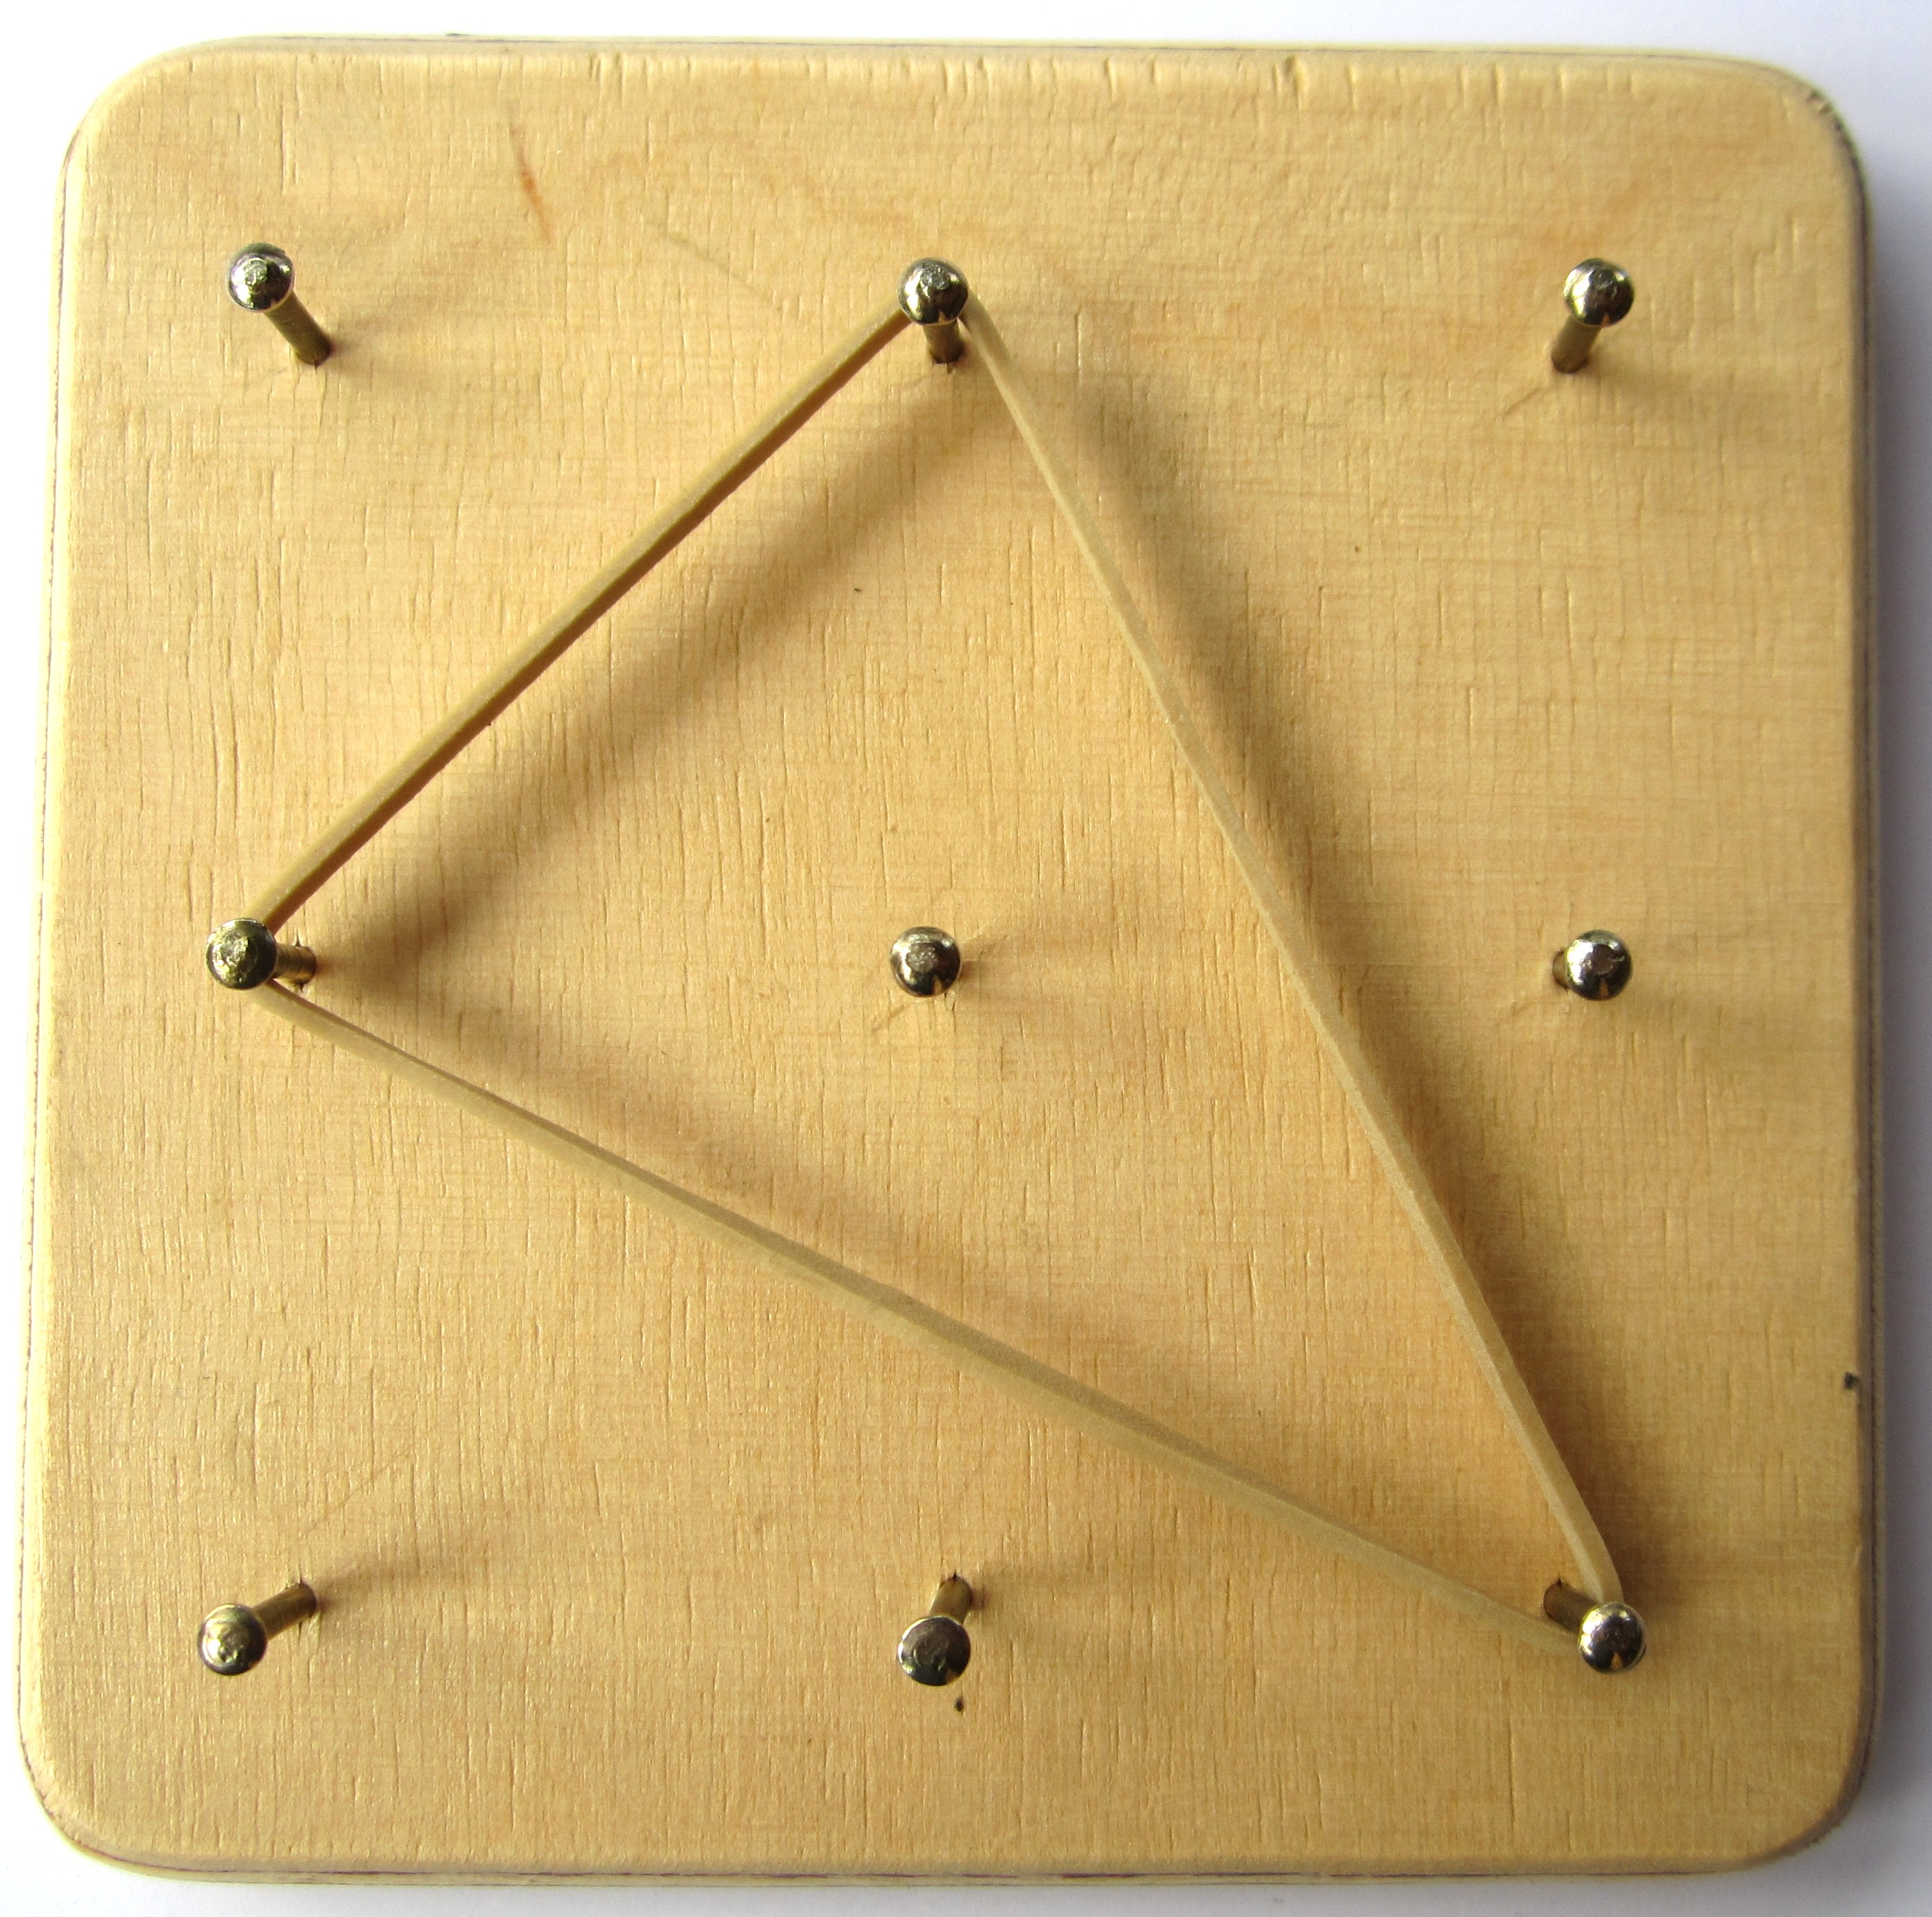
\includegraphics[width=.5\linewidth]{images/Geoboard}
\end{array}$
\end{center}
\caption{A simple 3x3 geoboard, with a rubber band stretched around several
pegs, forming a triangle.}
\label{fig:geoboard}
\end{figure}

The UCube (as seen on the left in \ref{fig:ucube1}) is the initial result of
this goal. The physical interface consists of a set of vertical ``towers'' that
are placed (and optionally re-placed) onto a grid of 4x4 evenly spaced nodes or
sockets, which act somewhat like the nails in the 2D geoboard. The towers
themselves contain four switches placed vertically along the tower, creating a
potential for 64 (4x4x4) distinct points to be activated. The towers are
``plugged in'' when placed into one of the 16 socket nodes, connecting them to
the underlying circuitry responsible for providing power to the towers and
relaying the state of each of the switches to the computer, via an Arduino
Mega\cite{ArduinoMega} microcontroller. Thus, when a tower is placed in a
specific node on the board and a switch is flipped on, a particular (x,y,z)
coordinate in three-dimensional space is activated and sent to a piece of
software on the computer. An abstracted illustration of the hardware system is
seen on the right in \ref{fig:ucube1_schematic}.

\begin{figure}[!ht]
\begin{center}$
\begin{array}{cc}
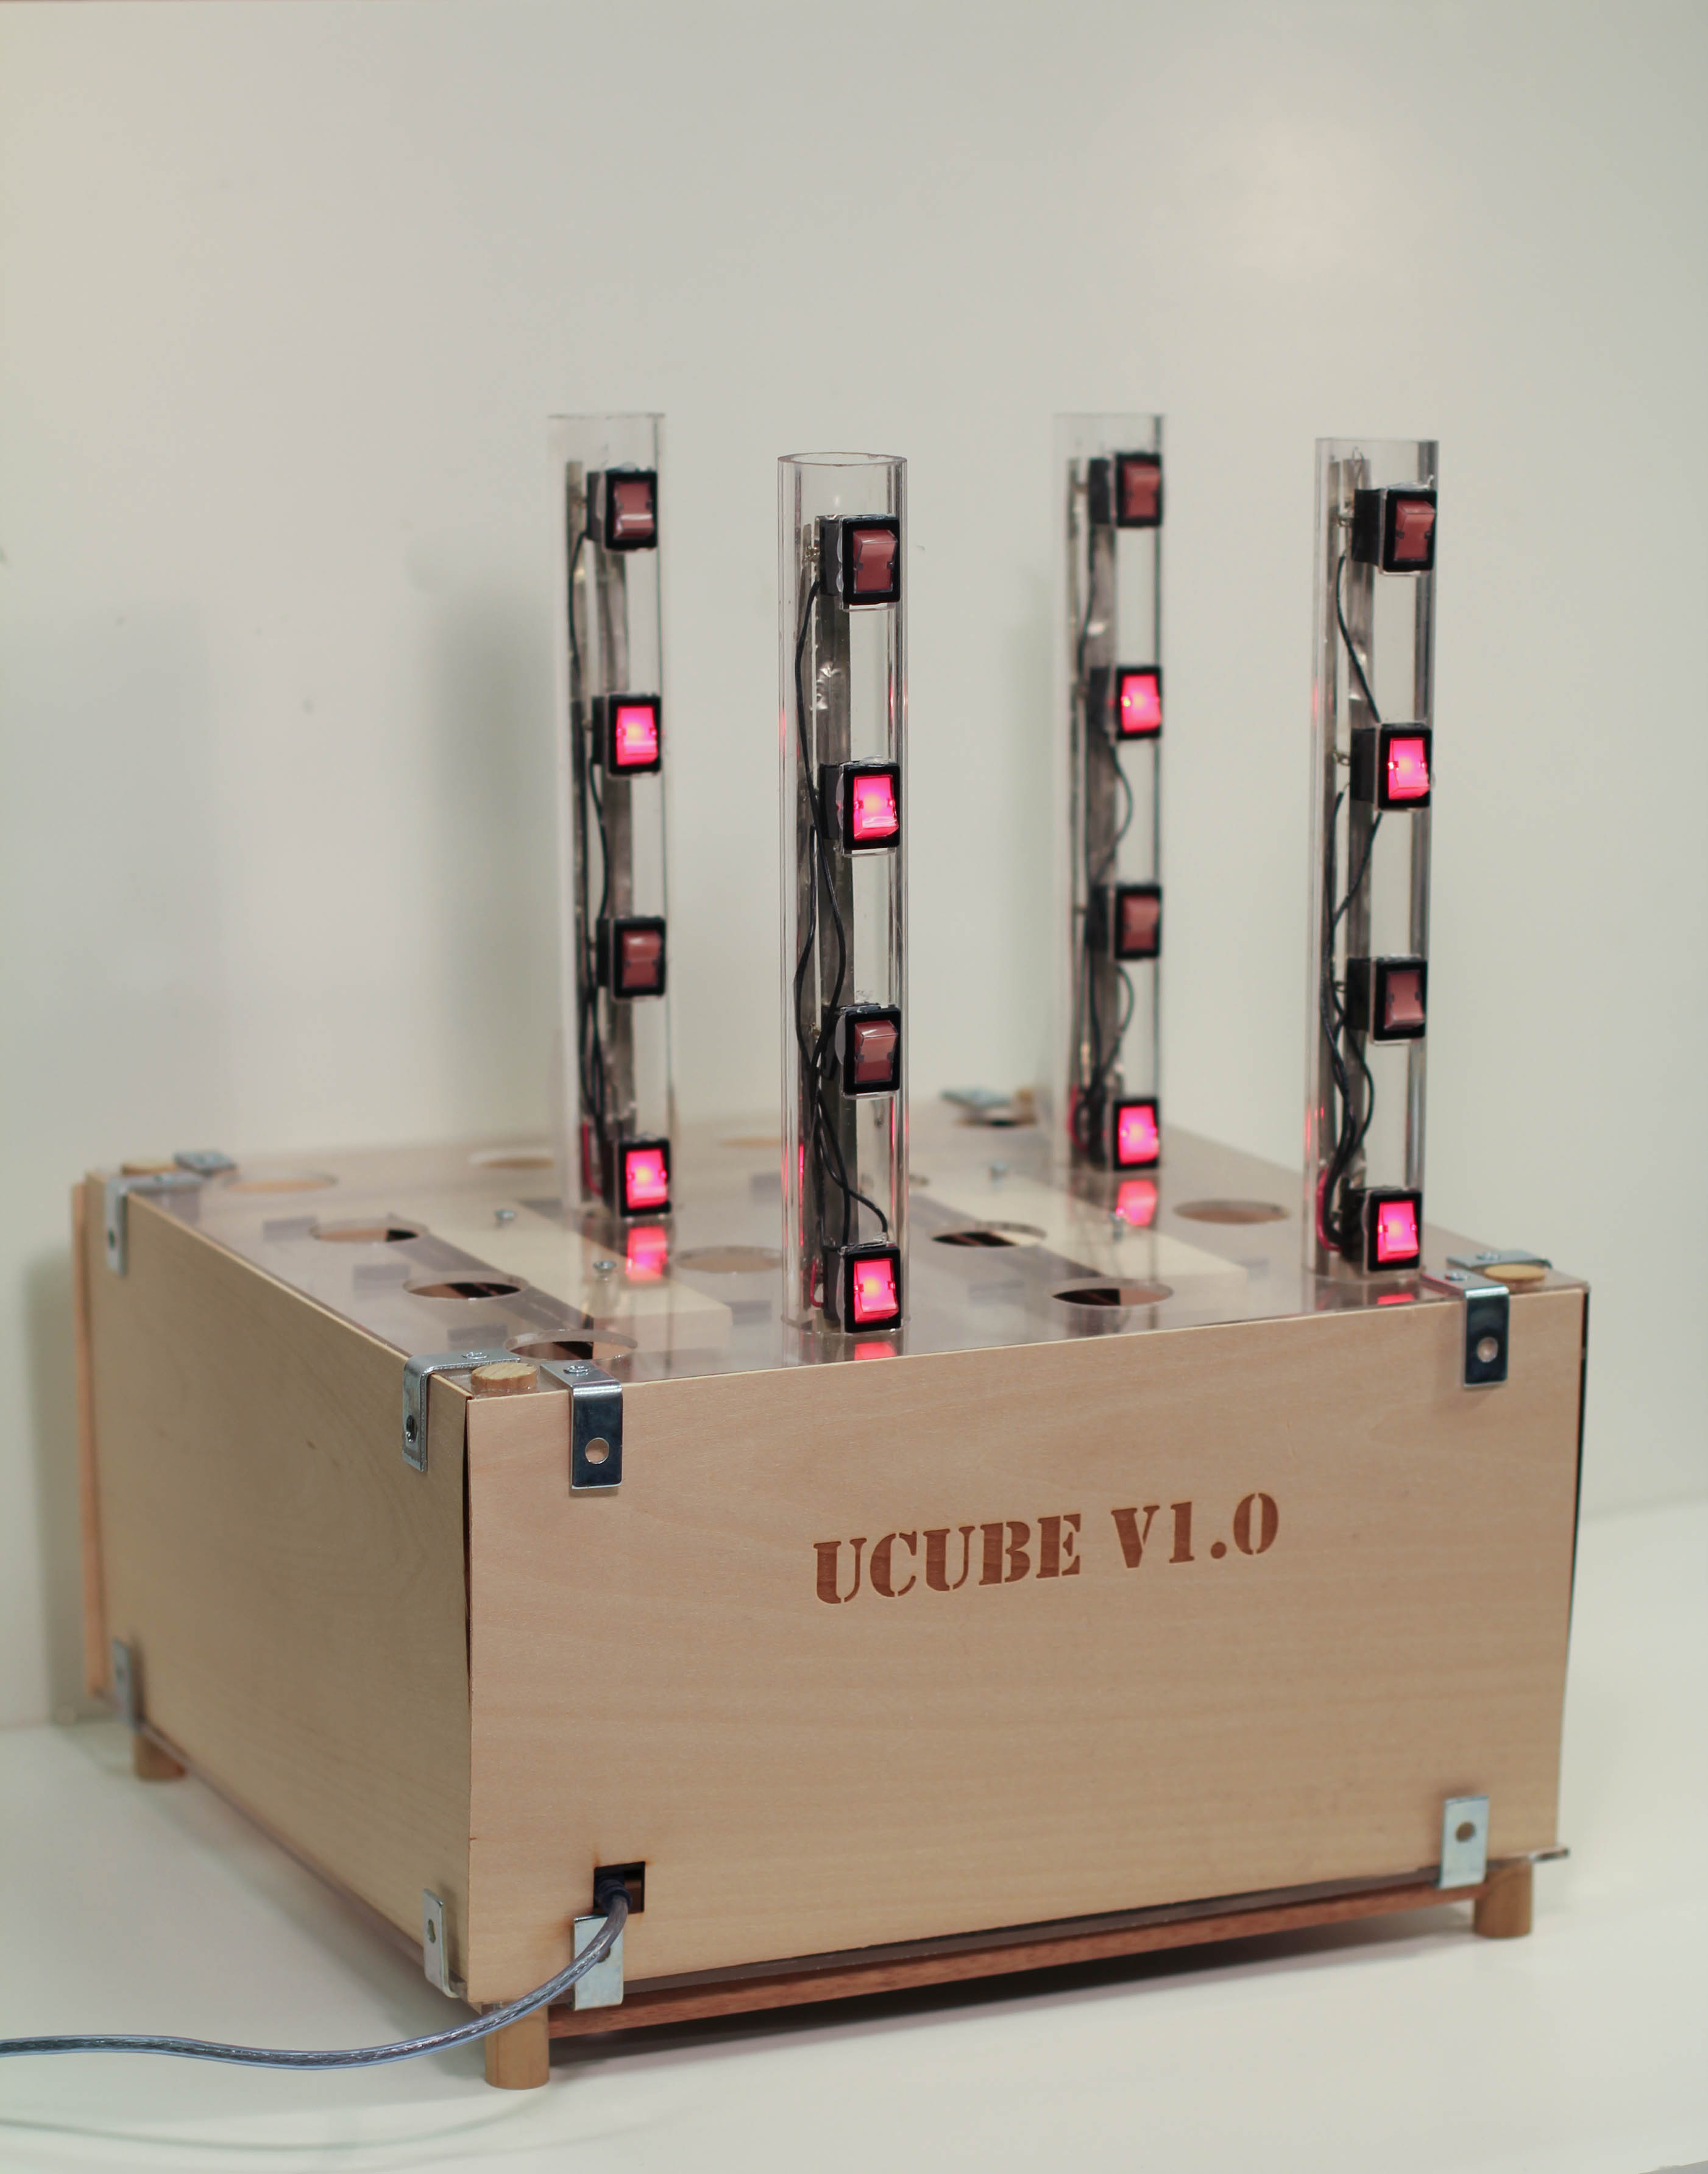
\includegraphics[height=3in]{images/UCube-3}&
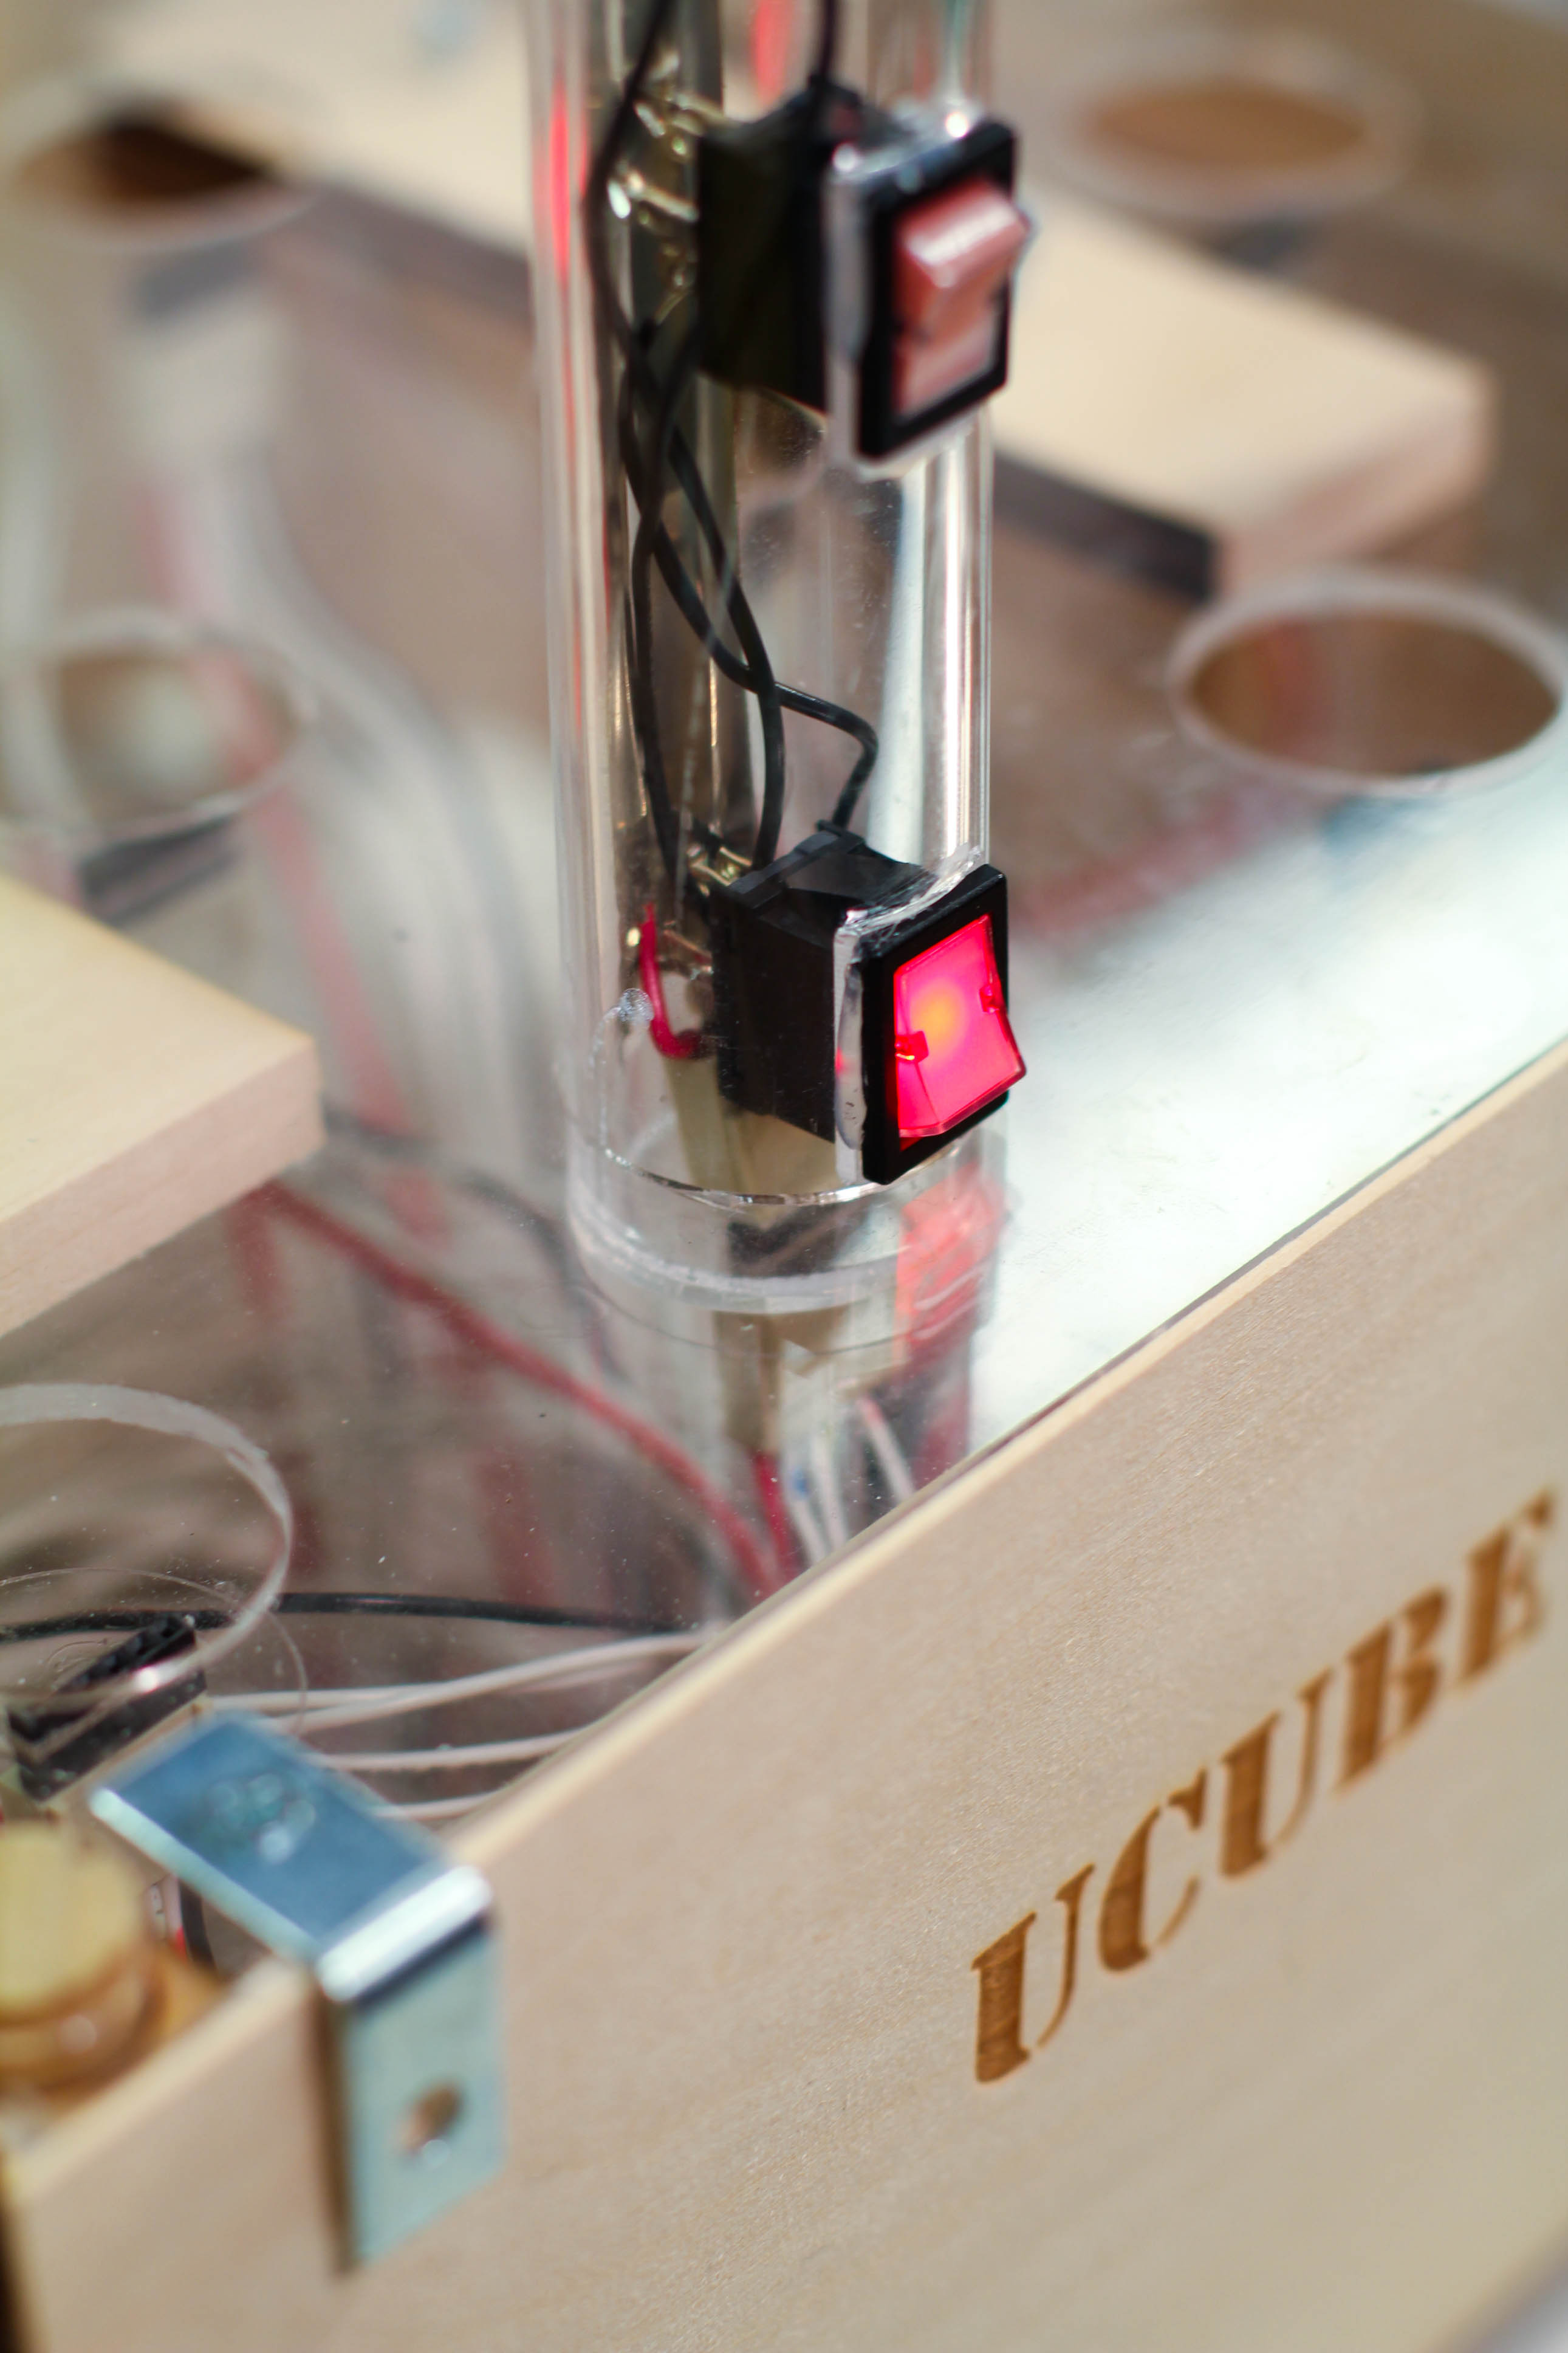
\includegraphics[height=3in]{images/UCube-4}
\end{array}$
\end{center}
\caption{Left: The UCube device, with four towers and eight lit switches,
representing (in one instance) the eight vertices of a cube. Right: A detail
view of one of the towers placed into the UCube modeling board with the bottom
switch lit.}
\label{fig:ucube1}
\end{figure}

Figure \ref{fig:ucube1} shows two views of the UCube interface. The picture on
the left shows the device, with four towers placed in an evenly spaced square,
with one ``board unit'' separating each tower. The lowest and third-lowest
switches on each tower are lit, marking eight active points. Thus we have eight
active points, spaced evenly in such a way to describe a cube of 2
``board-units'' in length if we were to take the convex hull of those points.
The photo on the right gives a detailed view of the UCube hardware. A tower has
been plugged into the board and its bottom-most switch turned to the ``on''
position. 


The UCube software (discussed more thoroughly later in the chapter)
takes the incoming coordinate data from the microcontroller and translates it
into a real-time visualization on screen. The graphical user interface centers
around a ``ghosted'' grid of all the potential points, with the active points
being highlighted. In the first version of the software, the interface also
provides a set of operations that can be performed on the set of active points
in addition to normal scene manipulations like zoom and rotate. These functions
are explained more thoroughly in the software section later in the chapter, but
to give a brief list, include: taking the convex hull of the point set (as
imagined in \ref{fig:ucube1}), creating a sequential path or knot through the
active points, exporting the convex hull or knot to .STL format for 3D printing,
drawing a (non-printable) spline through the active points, saving and loading a
shape, and editing the vertices of a convex hull via a click-and-drag interface.



% from IDC 2011 paper
% As a first step in discussing the UCube's role in spatial design�and in
% discussing the broader issue of children's three-dimensional design�this section
% is devoted to a more thorough description of the UCube and its operation.
% To begin with an overview, then: the UCube system is the combination of two
% elements: the physical input device of ``towers'' placed on a board, and the
% companion display software. These two systems work together to take the embodied
% actions of the user and display corresponding points and shapes on the computer.
% A sense of the scale of the device can be inferred from \ref{fig:cubev2}, which
% shows a photograph of a middle-school student holding a newly-placed tower in
% the UCube platform while pointing simultaneously at the desktop computer screen
% beside it.
% This photograph�which we will also return to in the discussion of pilot testing
% in a later section�reflects the essential nature of interaction with the device:
% points are designated in a spatial region provided by the platform, and then
% represented in real time on the computer screen. Thus, the UCube promotes an
% attention to the correspondence between the selected spatial points above the
% platform and the (more abstract) representation on the computer screen.

\subsection{Technical Implementation} 
The physical system for our first UCube prototype, as outlined earlier, consists
of a platform with a four-by-four grid of potential sites, each of which can
hold one tower with four switches, thus describing a 4x4x4 array of 64 potential
points. The platform structure consists of three different horizontal
``layers''. The top (or upper surface) layer is a clear 1/4'' acrylic square,
into which a four-by-four grid of circular holes has been laser cut in such a
way that the towers fit snugly. This layer of clear acrylic acts as a brace to
hold the towers upright, helps guide the pins from the tower into alignment with
the socket into which they must be placed, and ensures that the towers
themselves are resistant to being knocked over.

The next layer down holds a set of headers, six per socket (one each for power
and ground, and four input lines, one for each switch), which allow the towers
to ``plug in'' and connect to the rest of the circuit. Wires from the headers go
down to the bottom layer, which holds the breadboarded circuit and Arduino Mega
microcontroller\cite{ArduinoMega}. The header wires connect directly to the
breadboard, where each switch circuit runs through a 10K$\Omega$ resistor, and
then to a digital input pin on the Arduino Mega. When plugged in, the Arduino is
able to communicate (via asynchronous serial communication) the set of active
switches (and corresponding coordinates) to the computer through a USB cable.
\ref{fig:ucube1_schematic} depicts a schematic diagram of the UCube hardware.

\begin{figure}[!ht]
\begin{center}$
\begin{array}{cc}
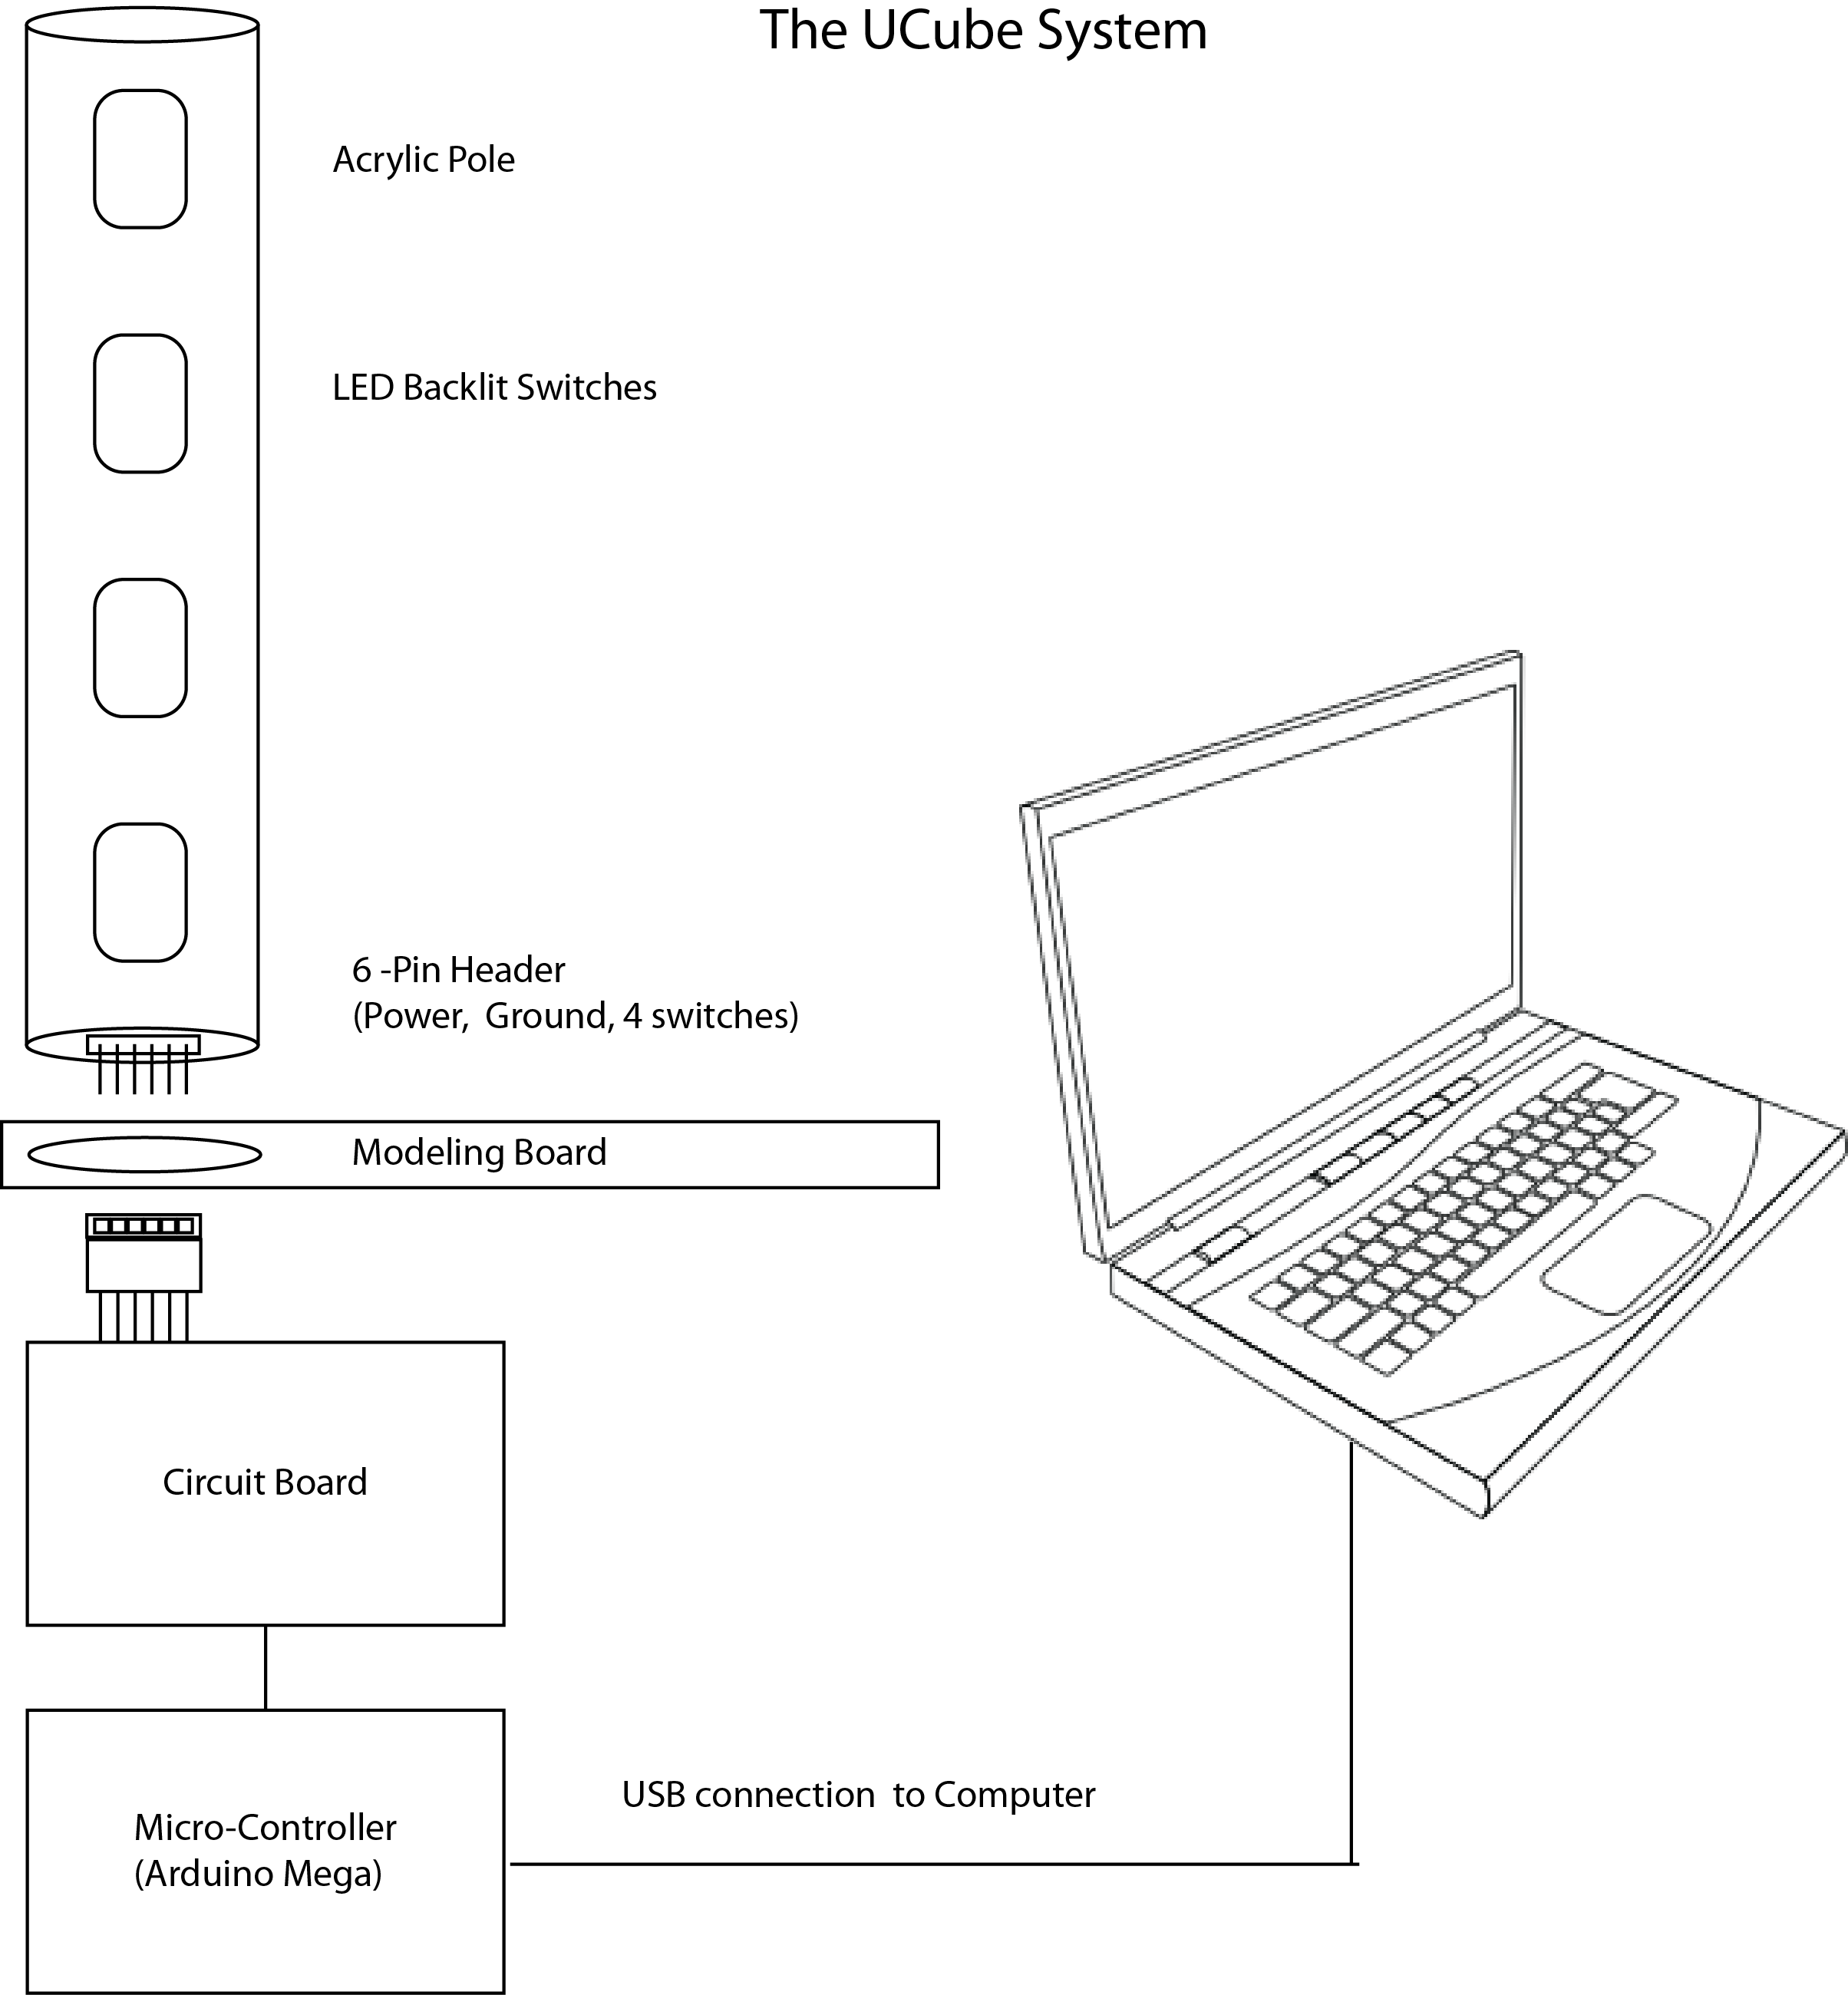
\includegraphics[width=.5\linewidth]{images/ucube_diagram}
\end{array}$
\end{center}
\caption{A schematic illustration of the UCube hardware.}
\label{fig:ucube1_schematic}
\end{figure}

The towers are made of transparent acrylic, cut from a 1'' diameter circular
tube. The towers were laser-cut in order to house the four switches and
corresponding circuitry elements. Four laser-cut rectangles are sized to allow
the back of each switch to be placed inside the tower while the faceplate
remains on the surface. The switched are backlit with in-built red LED's. Each
switch has a 270$\Omega$ current limiting resistor soldered between two of its
legs to protect the lighting element. Headers were soldered on to the power and
ground pins of the switch, and connect to a strip of conductive tape affixed to
the back on the inside of the tower (one can make this out somewhat in Figure
\ref{fig:ucube1}). The signal line from the switch (responsible for letting the
microcontroller know it has been switched) is soldered to a wire which reaches
down a six-pin header at the base of the tower. As the switches are LED-backlit
when active, it becomes more apparent which points are active as well as giving
a more accessible ``gestalt'' of the shapes being modeled. The luminosity also
allows for some potentially interesting applications in dimly-lit circumstances,
such as modeling constellations in a classroom or planetarium: in these
situations, the lights of the selected spatial points stand out especially
vividly.


\subsection{A Sample UCube Scenario}
As a sample scenario, imagine that we wish to create a triangular prism solid
employing the UCube. We can begin this process by selecting three points to form
a triangle; then, by placing two more towers and creating the same triangular
shape "shifted over" by two units (as seen on the left of \ref{fig:cubev1}) we
create the entire prism. Naturally, there might be many alternative pathways to
forming the same eventual shape: for example, we might begin by placing four (or
more) towers in the platform, and then experiment or fiddle with the chosen
lights to approach the eventual goal of creating our prism. Alternatively, we
might begin without any towers in the device at all: by placing our hands or
fingers above the device, roughly indicating where the prism should be, we might
then use our imagined locations as ``guides'', helping us to place the necessary
towers in the platform and select the correct lights for the vertices of the
prism.
In any event, having designed the prism using the UCube platform, and having
checked that it looks like the correct shape on the computer screen (as seen in
the center of \ref{fig:cubev1}), the final step is to export the shape into a
format suitable for 3D printer output. The UCube software, as noted earlier,
includes a feature for doing just this; and finally, we print out the prism, as
shown on the right in \ref{fig:cubev1}.

\begin{figure}[!ht]
\begin{center}$
\begin{array}{ccc}
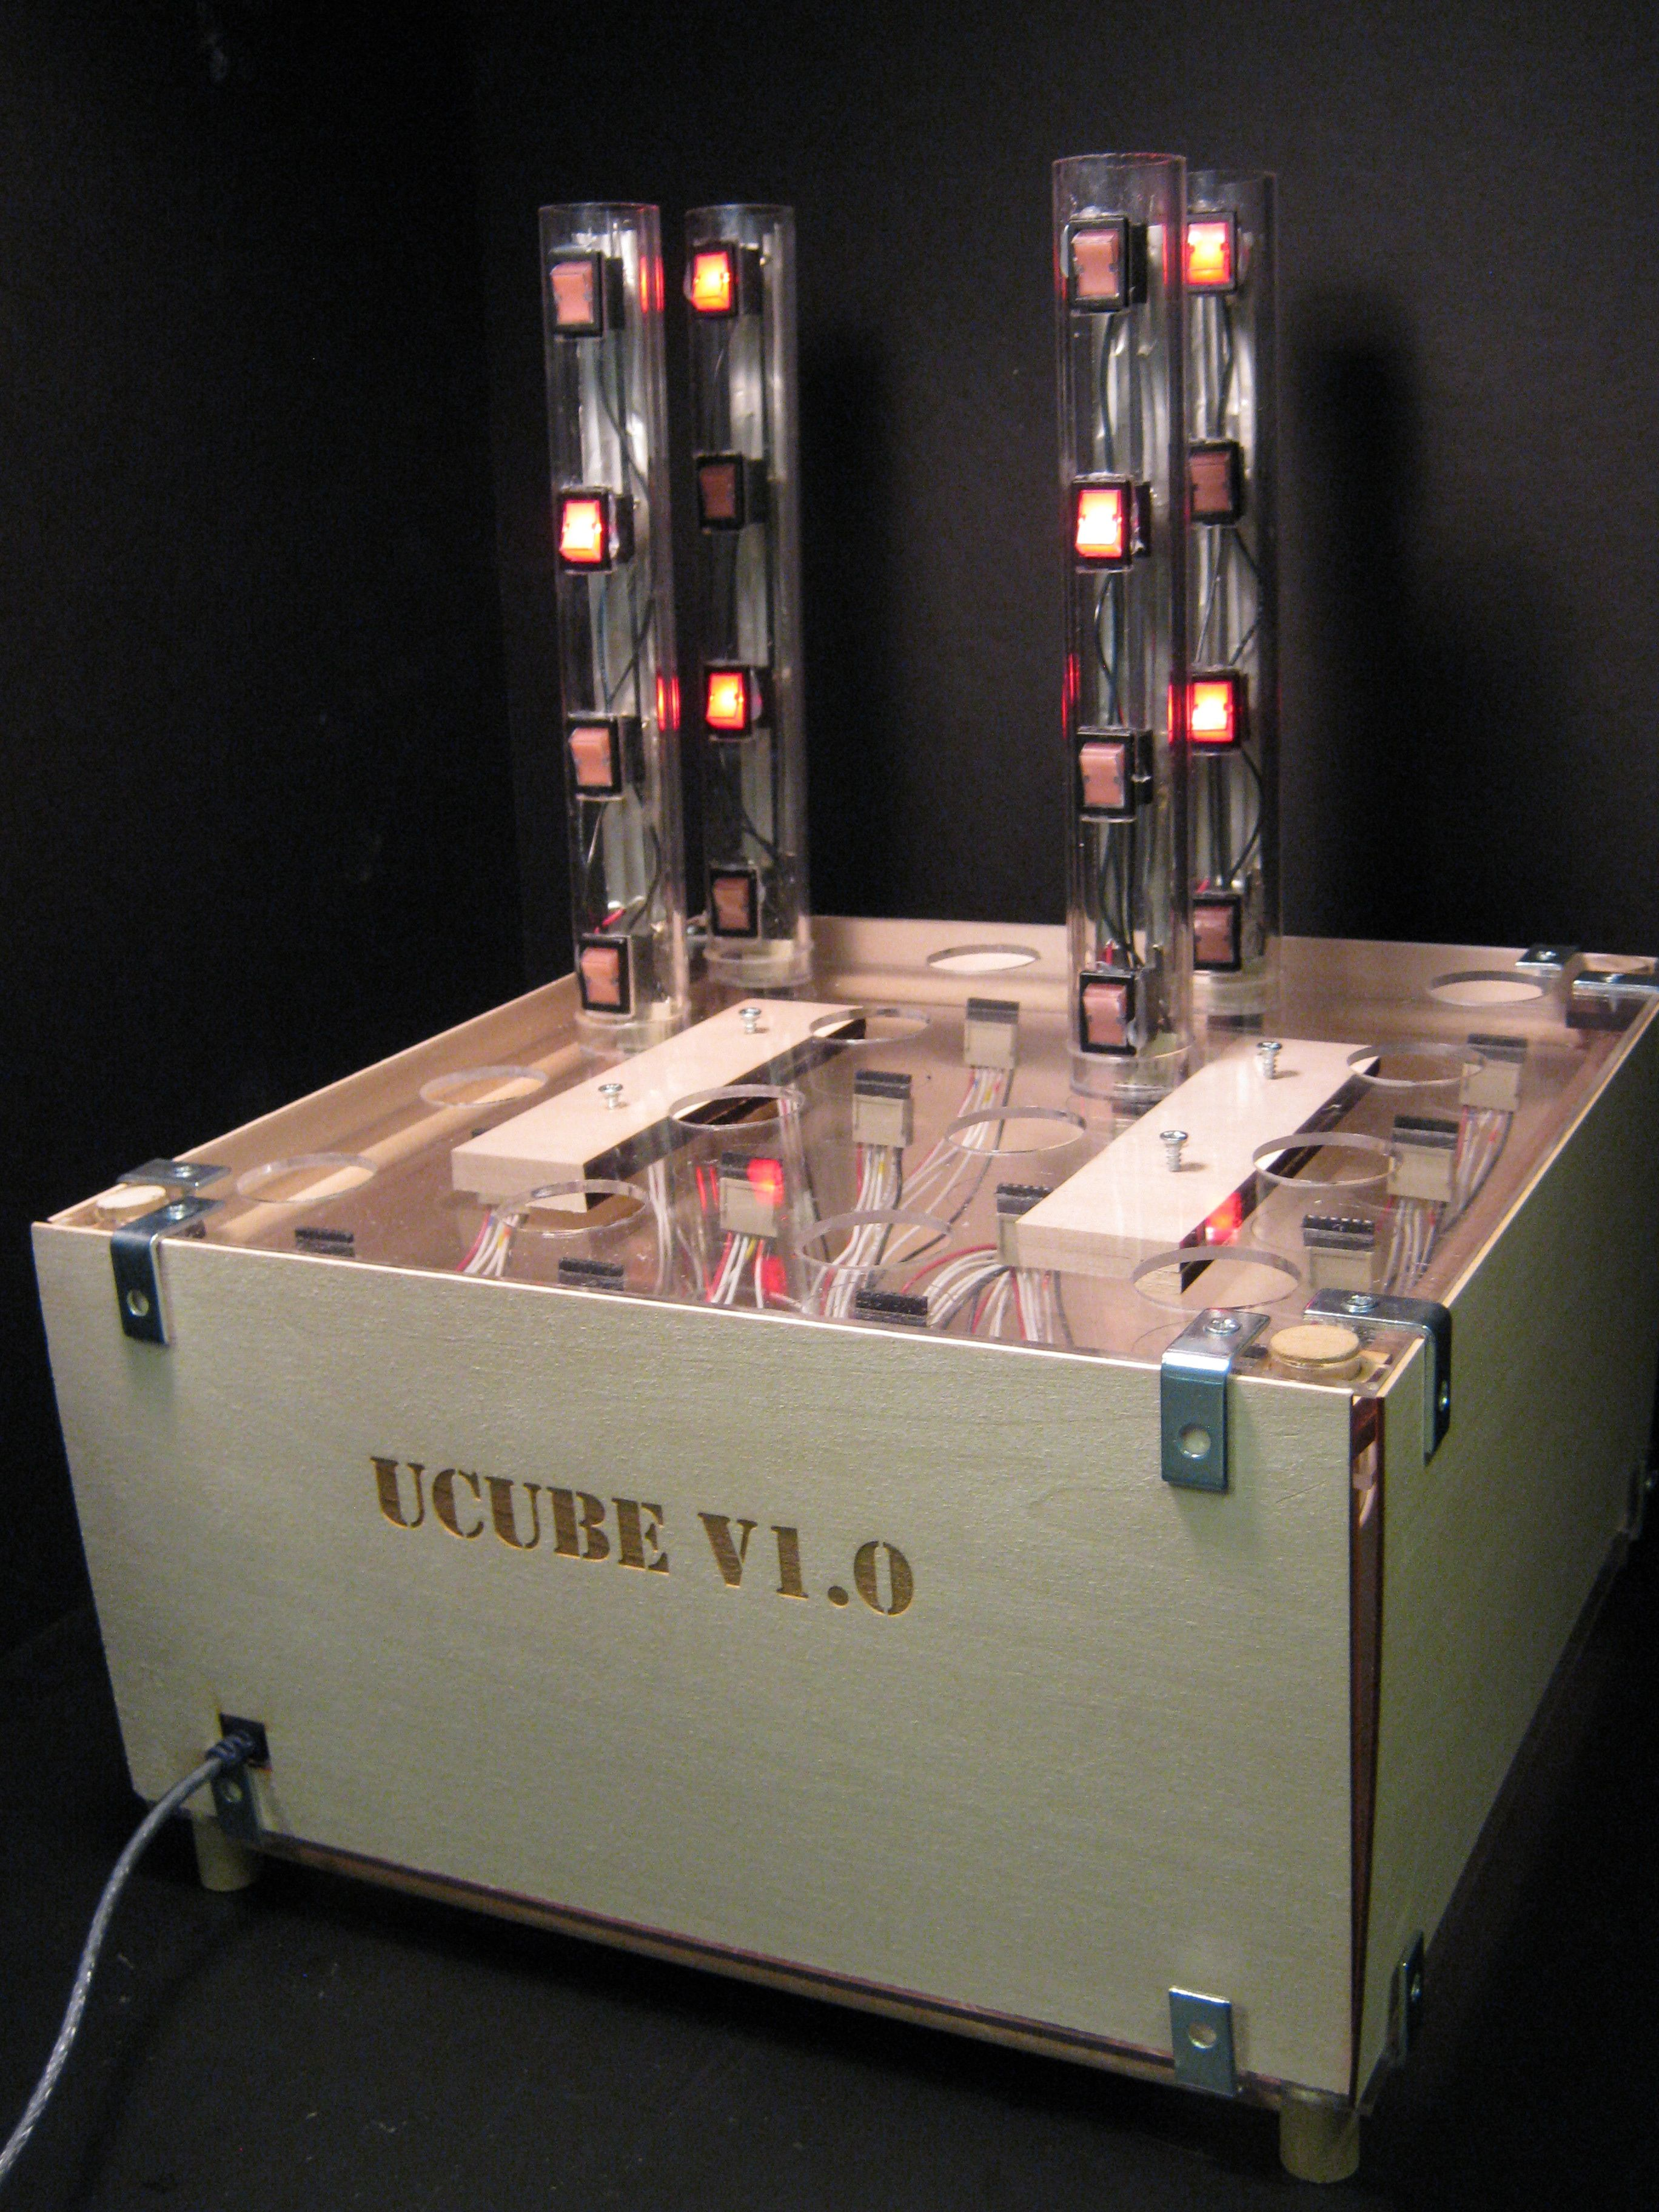
\includegraphics[width=.26\linewidth, height=2.3in]{images/ucube1_triPrism}&
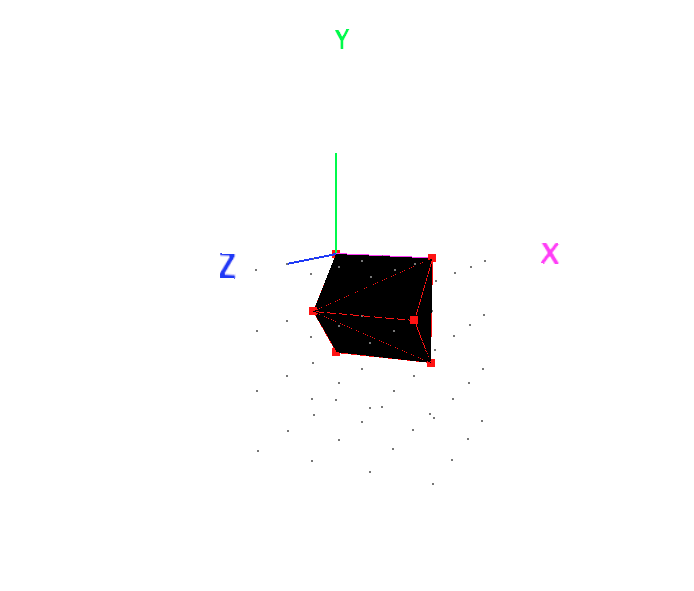
\includegraphics[width=.32\linewidth, height=2.3in]{images/ucube1_software} &
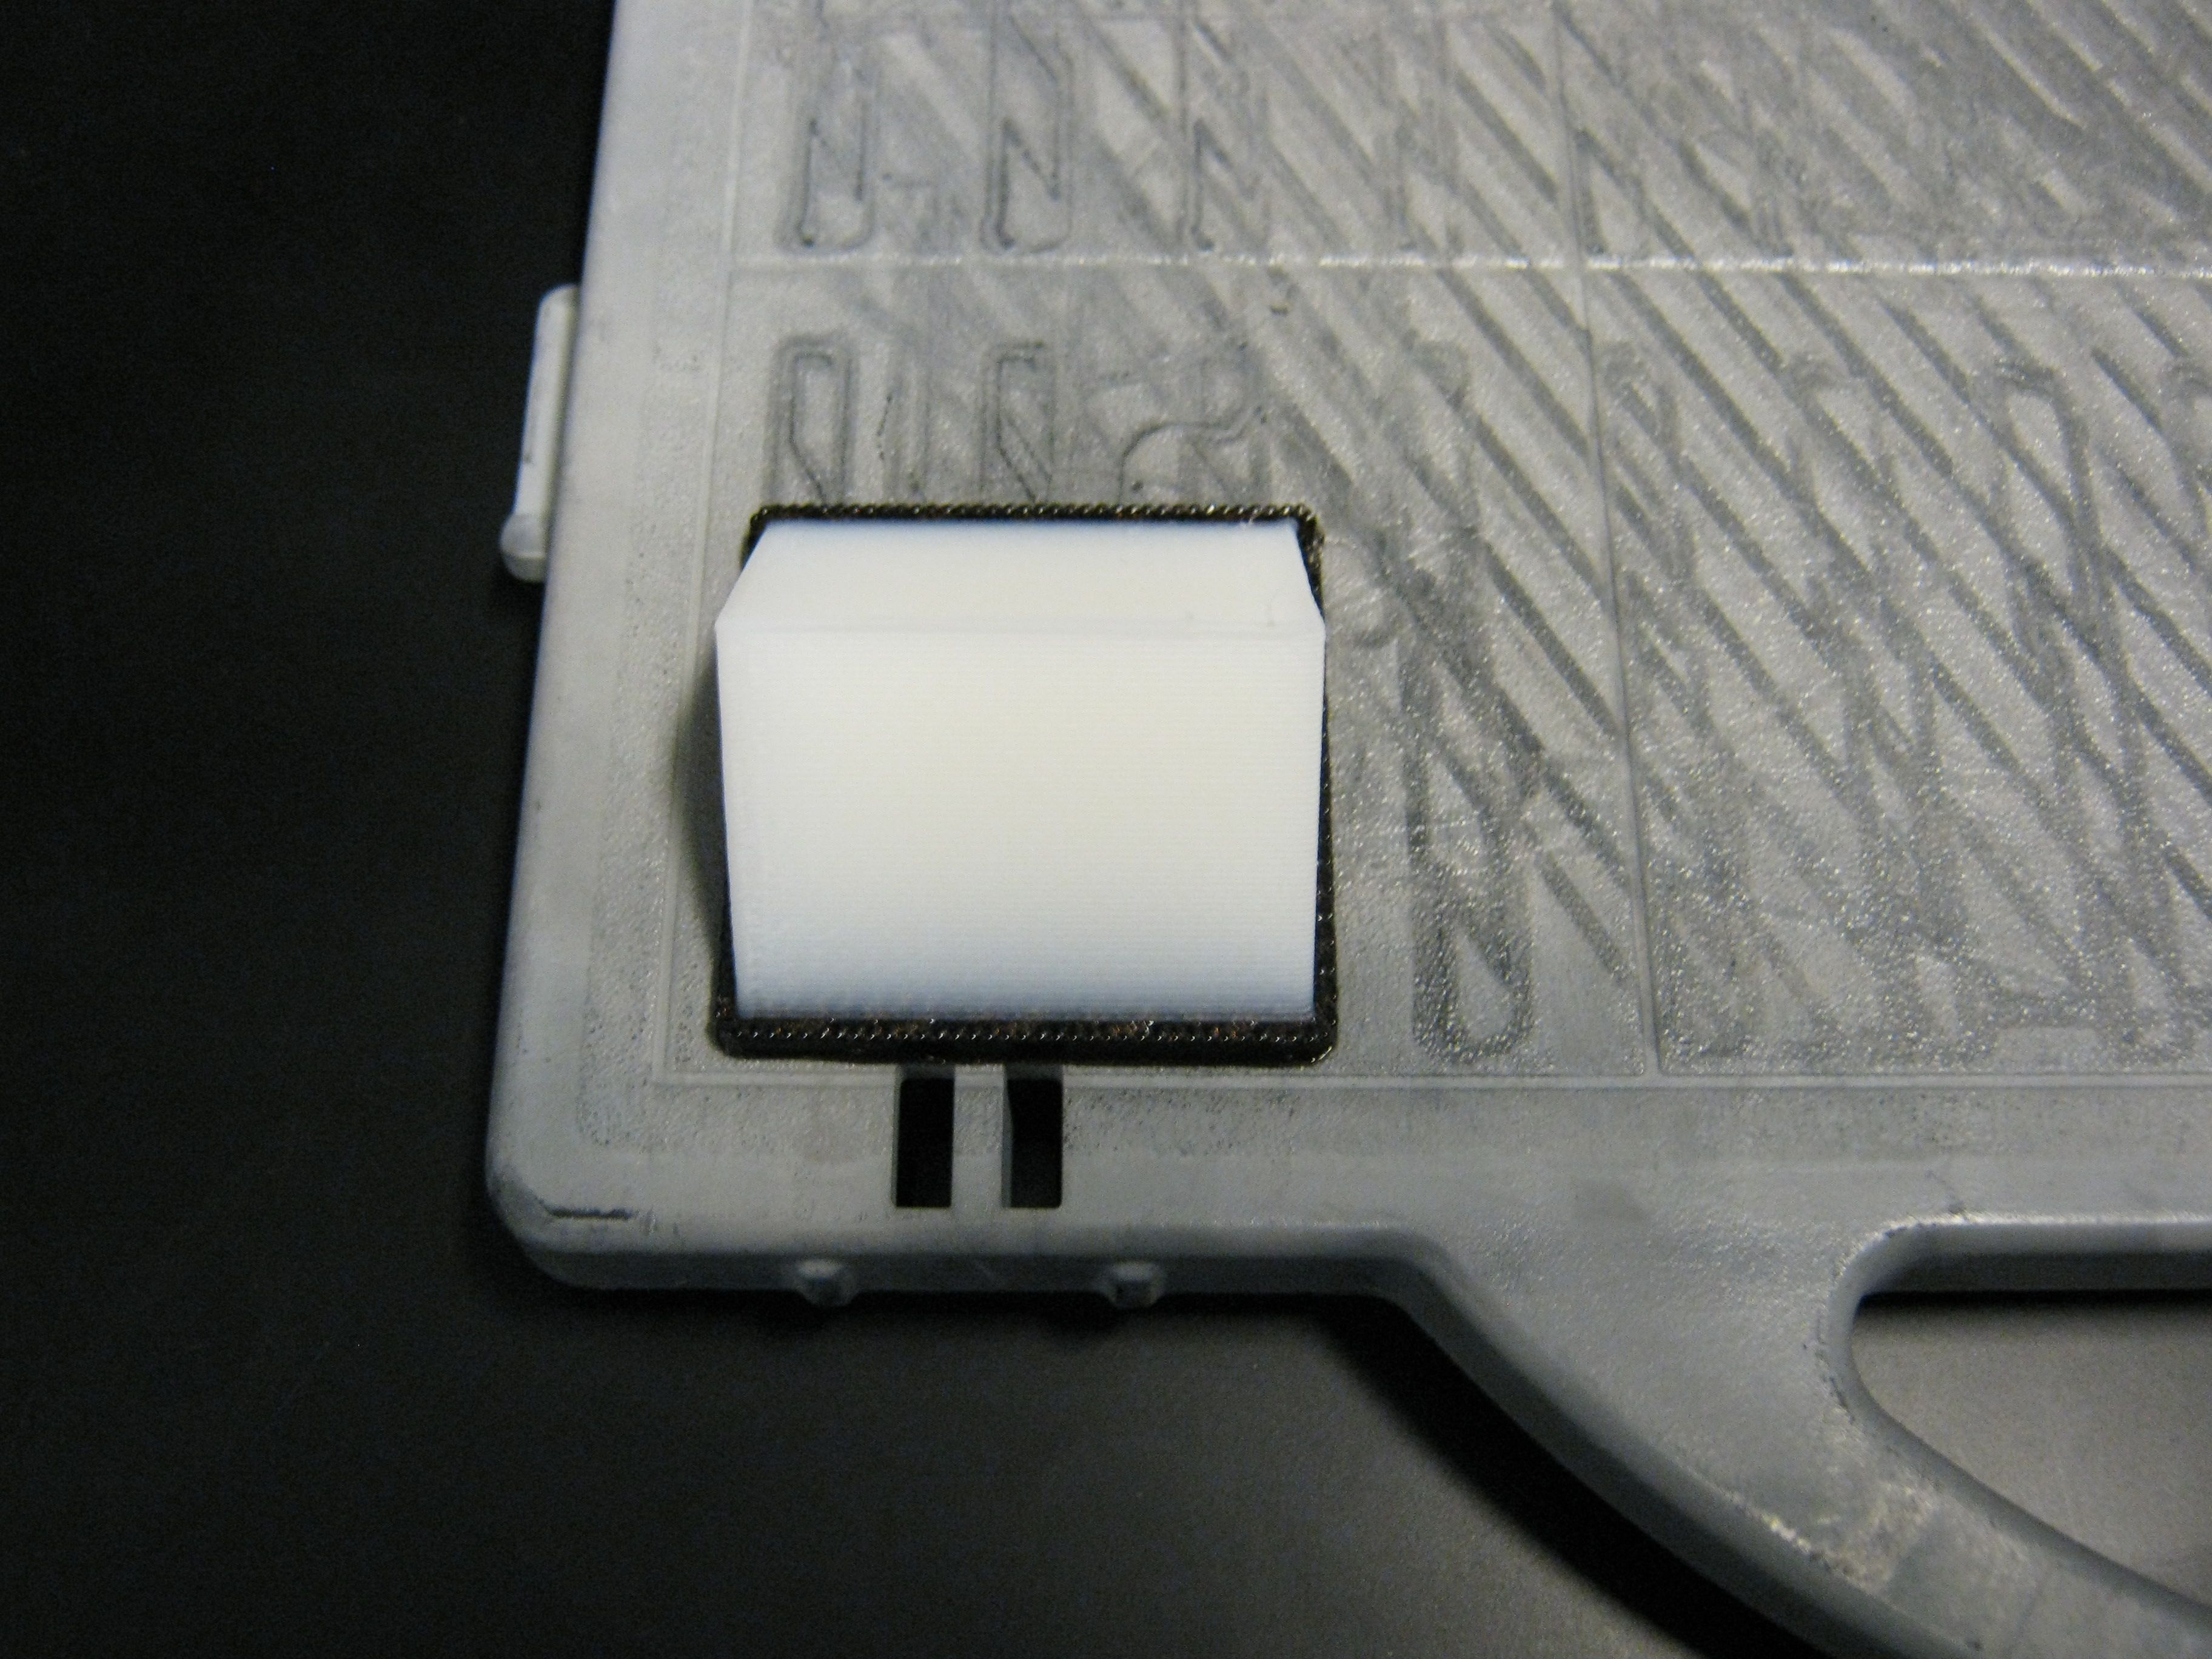
\includegraphics[width=.32\linewidth, height=2.3in]{images/IMG_0425}
\end{array}$
\end{center}
\caption{Left: The UCube device, with four towers and six lit switches,
representing the six vertices of a triangular prism. Center: An early version of
the UCube software, representing the convex hull formed with the six active
points from the picture to the left. Right: The resultant 3D print, exported
from the software to a 3D-printer friendly format.}
\label{fig:cubev1}
\end{figure}

\subsection{Limitations}

The astute reader will have picked up on some of the more obvious limitations of
the early system: as a three-dimensional modeling device, it is quite limited in
the scope of things it can effectively model, certain geometric shapes are
impossible to model on an integer lattice (a dodecahedron, for instance), a
4x4x4 resolution is clearly insufficient for complex shapes, and the inability
to create curved surfaces precludes most ``natural'' objects (such as human
faces) from being represented in a life-like manner. It is thus important to
differentiate this system (and the others mentioned in this chapter) from a
``professional'' 3D modeling system; our focus is on ease of use for novices, to
provide a visual and tactile bridge between 2D and 3D worlds, and to provide a
simple way to create shapes suitable for 3D printing. Even so, this does not
preclude us from attempting to make a more powerful, expressive, and stable
interface to present to users.



\section{SnapCAD}

Based on the feedback and observations from the two user studies we performed
with the UCube (discussed in chapter 4), a second, more powerful instantiation
of the UCube has been created. Called SnapCAD (formerly known as UCube v2) this
next generation device consists of a total input space of 7x7x7 points, forming
343 distinct coordinates (as opposed to the 64 points of the UCube). We focused
on two main design goals with the SnapCAD: greater expressive power and greater
stability in the system operation.

\subsection{Technical Implementation}
To start with system stability, then; custom printed circuit boards have
replaced loose wires, the towers are designed in Rhino\cite{Rhino} and 3D
printed to safely and securely house the towers, which are in fact printed
circuit boards of their own. Instead of a rickety housing, the top layer is
1/2'' acrylic which was milled on a CNC machine to precisely fit the newly
designed towers. The sides and bottom are hand-crafted wood, with channels cut
to allow the top and circuit board layers to easily slide in and out. The frame
is not glued on one side to allow for repair and maintenance. This side is
secured by custom metal brackets and screws. Each socket has its own printed
circuit board, held firmly in place by zip ties around a latticed acrylic layer
underneath the boards. The system has since traveled to the Denver Art Museum,
the Computer Clubhouse in Lakewood, Colorado, and ridden around in the back of
several cars without mishap (not to mention roughly 20 hours of user testing by
eager adolescents).

\begin{figure}[!ht] 
\begin{center}$
\begin{array}{cc}
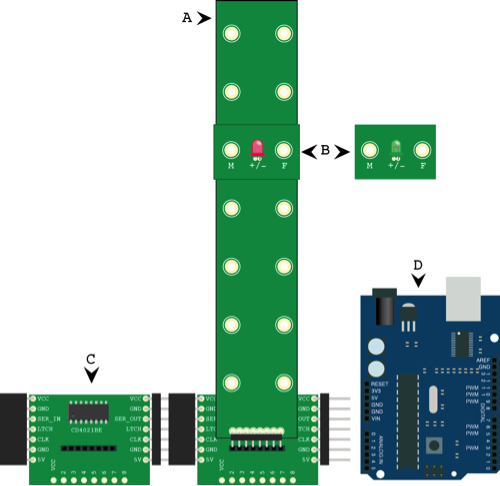
\includegraphics[width=.45\linewidth]{images/snap_schematic}
\end{array}$
\end{center}
\caption{A schematic of the SnapCAD technical design, showing a sample tower
(A), LED light element (B), shift register board (C) and Arduino (D). The Arduino
microcontroller's role is to send coordinates (and colors) of the LED lights,
once placed, to a desktop computer. A fuller description of this schematic is
provided in the accompanying text.}
\label{fig:snap0}
\end{figure}

The goal of expressiveness was met in two ways; by increasing the possible input
space from 64 points to 343, and by designing a system that allowed for each
point to be activated by more than one color of LED - effectively allowing for
multiple shapes to be modeled at once, or multiple ``players" to interact with
the board at once. Both of these solutions required changes in both hardware and
software from the UCube. Working on the scale of multiple hundreds of inputs
necessitated the design of custom circuit boards to relay information
effectively to the microcontroller. The Arduino Mega has only 54 digital
input/output pins, far too few to assign each line directly to an input, even if
one wanted to deal with tracking 343 i/o lines (which we most certainly did
not). Instead, we designed a circuit board around an input shift register chip
from Texas Instruments - the CD4021BE - that could effectively provide eight
more input lines per chip and operate with the Arduino's ATMega 328 Serial Peripheral
Interface (SPI) protocol, which requires only three lines from the Arduino. By
breaking out the pins on the CD4021BE so that they could be chained together (by
aligning the serial output of one chip to the serial input of the next chip,
while also passing along the latch and clock signals, the other two lines
necessary for the SPI to work)\footnote{We understand this section is somewhat
technical. A great introduction to using shift registers in this way can be
found at: http://www.arduino.cc/en/Tutorial/ShiftIn}. By arranging 49 of these
daisy-chained boards in a 7x7 grid, we had the framework to read in from 343
inputs in real time. Only one more problem had to be solved: at around 35
connected shift registers, we exceed what is called the ``fan-out'' of the
Arduino microcontroller - the number of connected input gates that a given pin
on the Arduino to drive a current load into. To get around this problem, the
clock and latch signals are put through a set of two ``buffers'' - in our case
CD4049BE inverting hex buffers - which can used for logic level conversion (the
inverting part, which we do not need, hence the second inverting buffer), but
also as a ``boost'' to drive the signal farther. One set of buffers was enough
to get our signals to the computer reliably.

This change in scale also meant rewriting most of the modeling software to
effectively handle the greater expressiveness of the physical system. The astute
reader may have noticed that while the CD4021BE adds eight inputs per board, our
system calls for a 7x7x7 array - so what were we to do with the extra input? The
dilemma actually ended up solving several problems; in the UCube firmware each
input triggered an (X,Y,Z) coordinate to be send out the serial port - by
switching to shift registers over SPI, we are limited to one character per input
- either a 1 or a 0. Normally, a serial string can be delimited in software by
looking for certain characters at the beginning or end of a communication, and
parsed accordingly, but we only had a string of 343 0's and 1's. Given that
most of the sockets would be returning a zero most of the time, by tying the 8th
input line high we could count characters and check for a ``1'' every eighth
character to ensure the serial string was correct - and since we were isolating
this character anyway, it was simple to throw it away afterwards and thus be
left with only the sets of seven digits describing the state of the inputs. The
problem of generating the proper coordinates from the input stream was then a
matter of creating a ``lookup table'' where the $nth$ character in the input
string array was the $nth$ element in an array of 3D coordinates.

\begin{figure}[!ht] \begin{center}$
\begin{array}{cc}
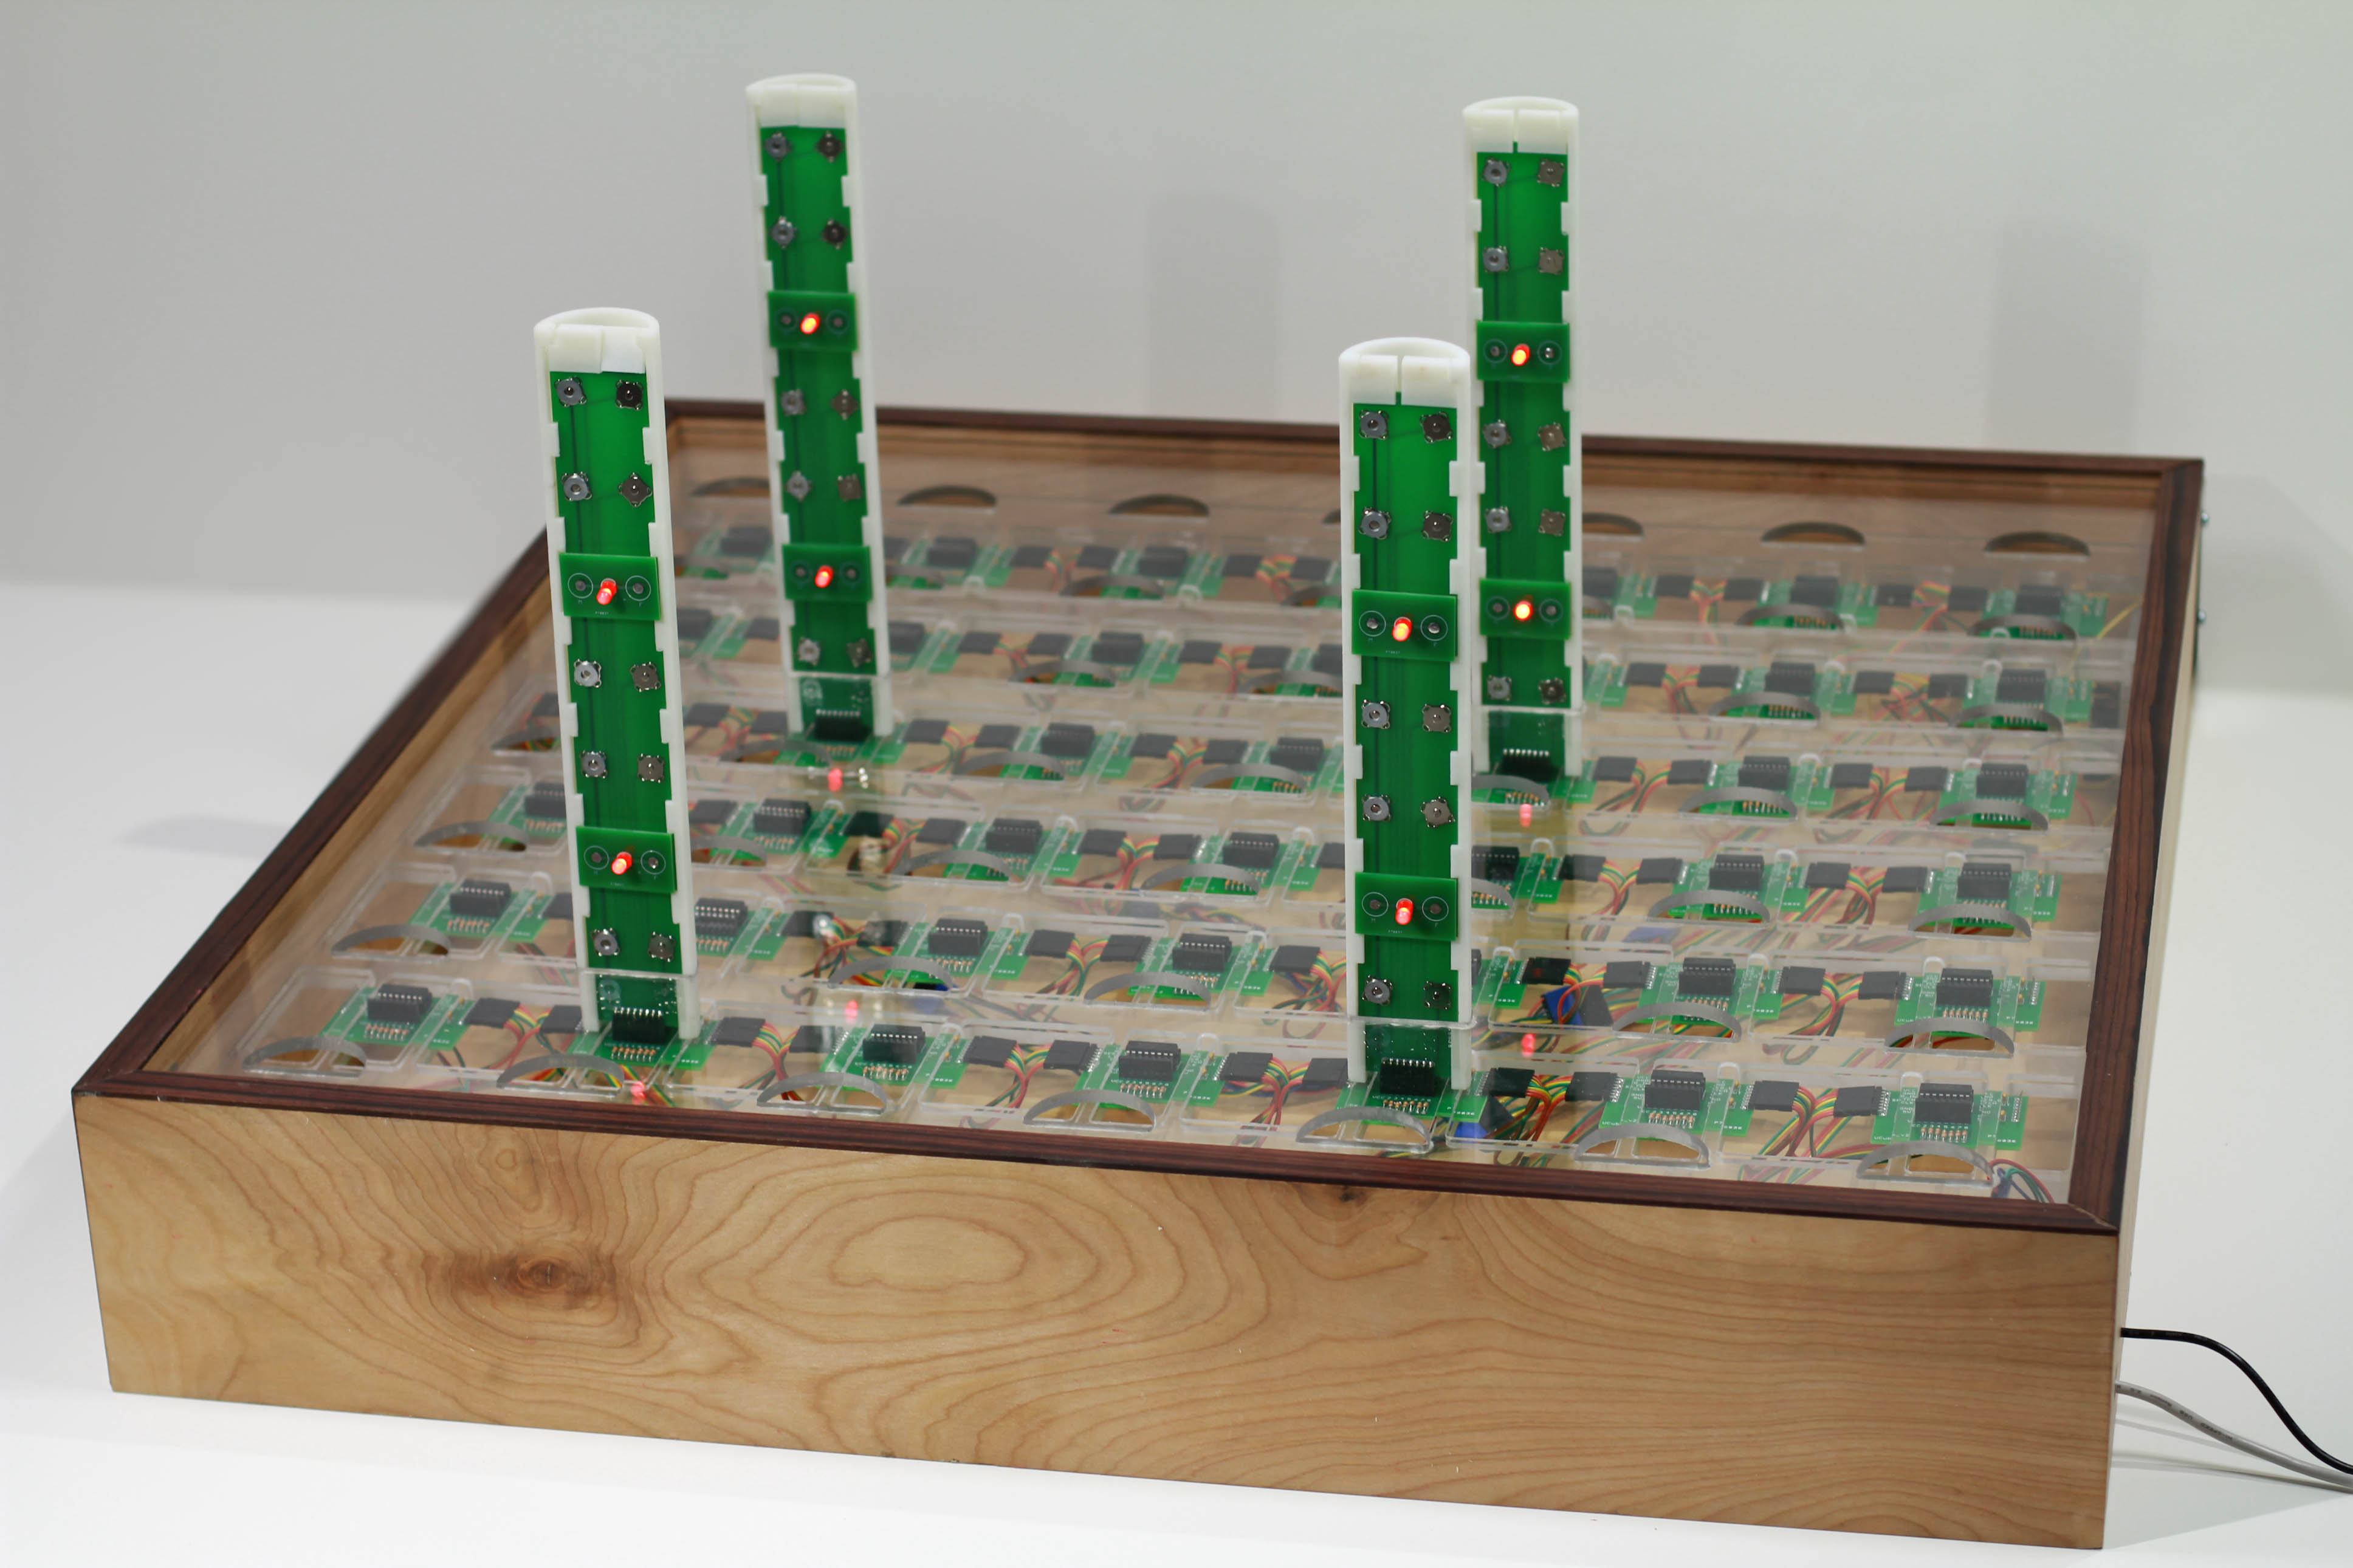
\includegraphics[width=.45\linewidth]{images/BeatriceFinal-9}& 
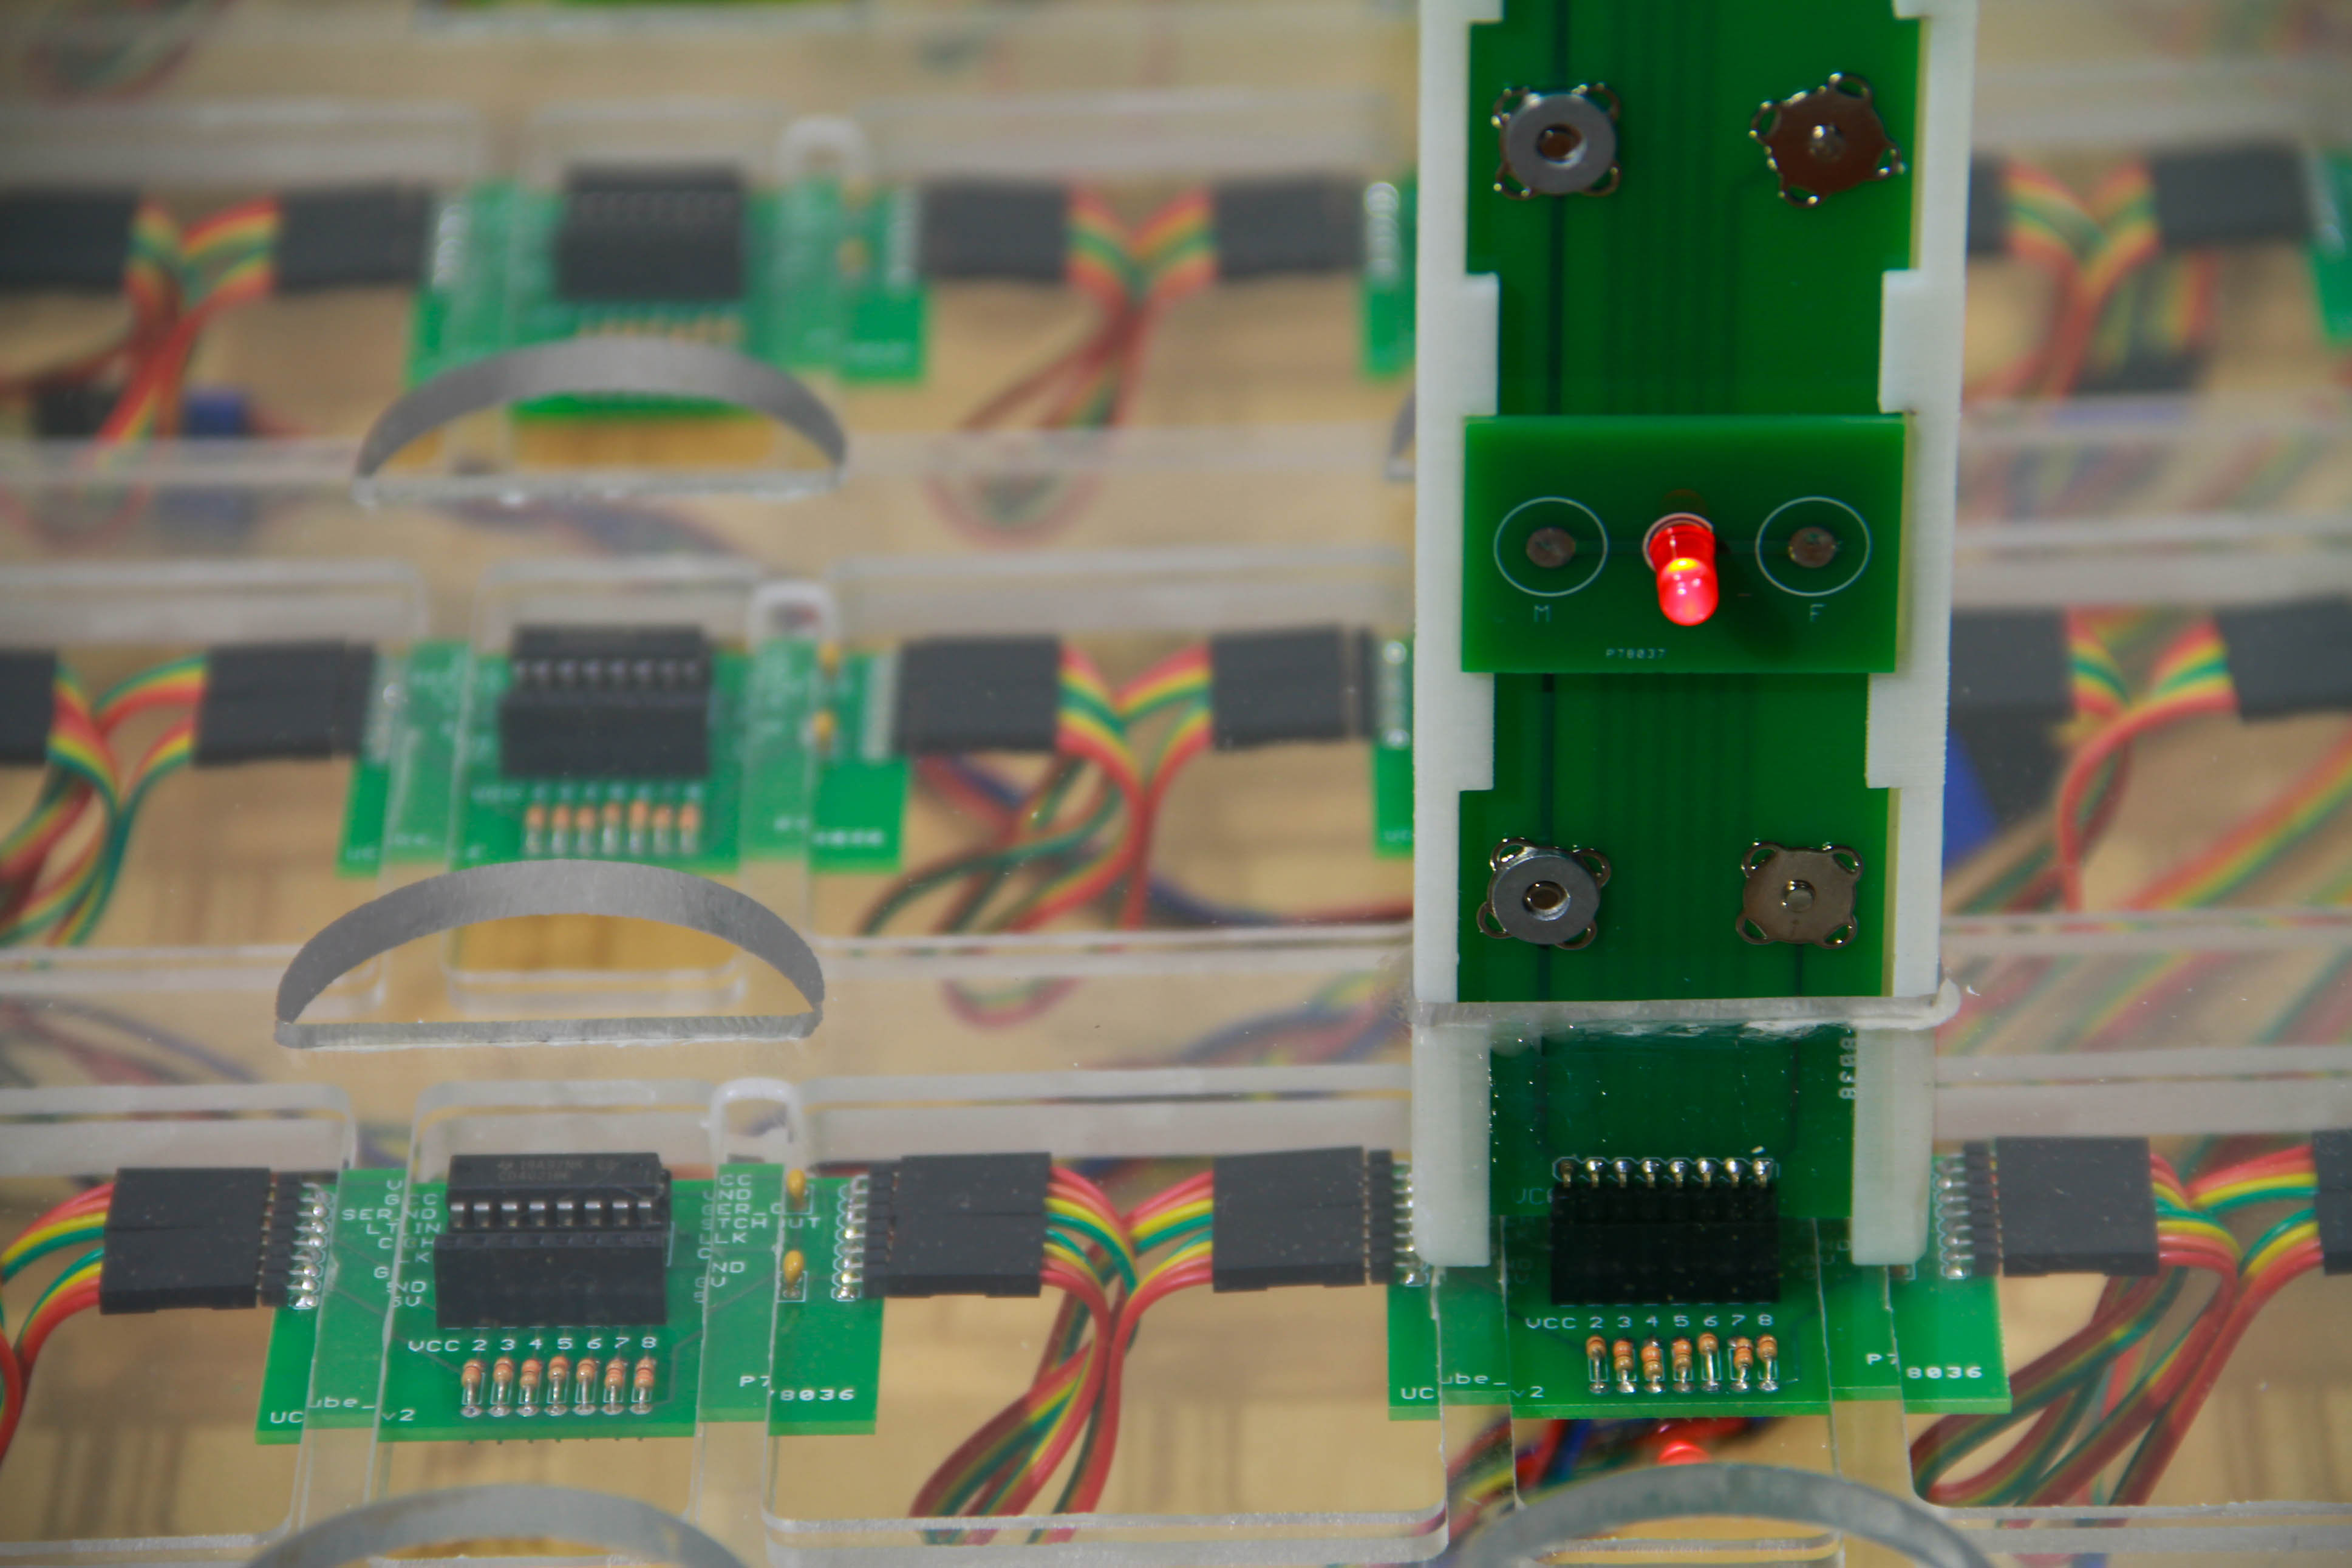
\includegraphics[width=.45\linewidth]{images/BeatriceFinal-14}
\end{array}$
\end{center}
\caption{
Left: the SnapCAD interface, showing four towers with two red LEDs each,
arranged in cube-like configuration. Right: a detail of the SnapCAD hardware -
the PCB tower is housed in a 3D-printed shell, which plugs into one of a chained
set of shift-register boards. The LED boards snap on to the towers via
conductive magnetic snaps.}
\label{fig:snap1}
\end{figure}

The other enhancement to the expressive power of the SnapCAD design is the
ability to use each socket in each tower with more than one color of LED. In
in order to make this a possibility, we had to find a way to make the LEDs
detachable from the tower and ``swap-able'' with other colors. This was achieved
by soldering conductive magnetic snaps directly into the circuit boards
themselves; the magnets act to both attach LEDs to the tower, but also to close
a circuit and light up the LED. We used snaps and not just simple magnets
because LEDs are polarized - they have only one correct orientation - and snaps
have a male and female part that could be used to indicate the correct
orientation. This multi-color capability can be seen in Figure \ref{fig:snap2}.

This ability to swap out different colors of LEDs not only results in the
ability to represent multiple shapes at once, but for the SnapCAD to become a
platform for all manner of multi-player interactions (e.g. games, puzzles, shape
matching contests), with each ``player'' assigned a unique color. To this end,
we have created a simple ``3D Tic-Tac-Toe'' implementation on the SnapCAD, and
imagined a sample scenario, explained in the next section. The SnapCAD version
of the software includes this ``multi-payer" ability as well as some additional
changes that include supporting multiple but separate convex hulls of different
colors, the ability to create and export shapes created from the minimal
spanning tree of a set of input points, and the ability to adjust the width of
the segments in the knot/path and minimal spanning tree modes.
The click-and-drag editing mode includes the knot/sequential path and minimal
spanning tree modes as well as the convex hull mode. We also adjusted the
knot-forming algorithm to handle paths that cross or self-intersect, as well as
providing a ``close knot'' button to complete a circuit in a shape, allowing for
even more kinds of 3D-printable objects.

% While significant work was been
% done to bring the UCube and SnapCAD to their current states, we believe not only
% that there is room for additional improvements to be made, but that, as opposed
% to focusing on a incremental but essentially similar interface as the subject of
% a thesis, it is far more intellectually interesting to focus on a class of
% objects that demonstrate multiple incarnations of a set of ideas.

\begin{figure}[!ht] \begin{center}$
\begin{array}{cc}
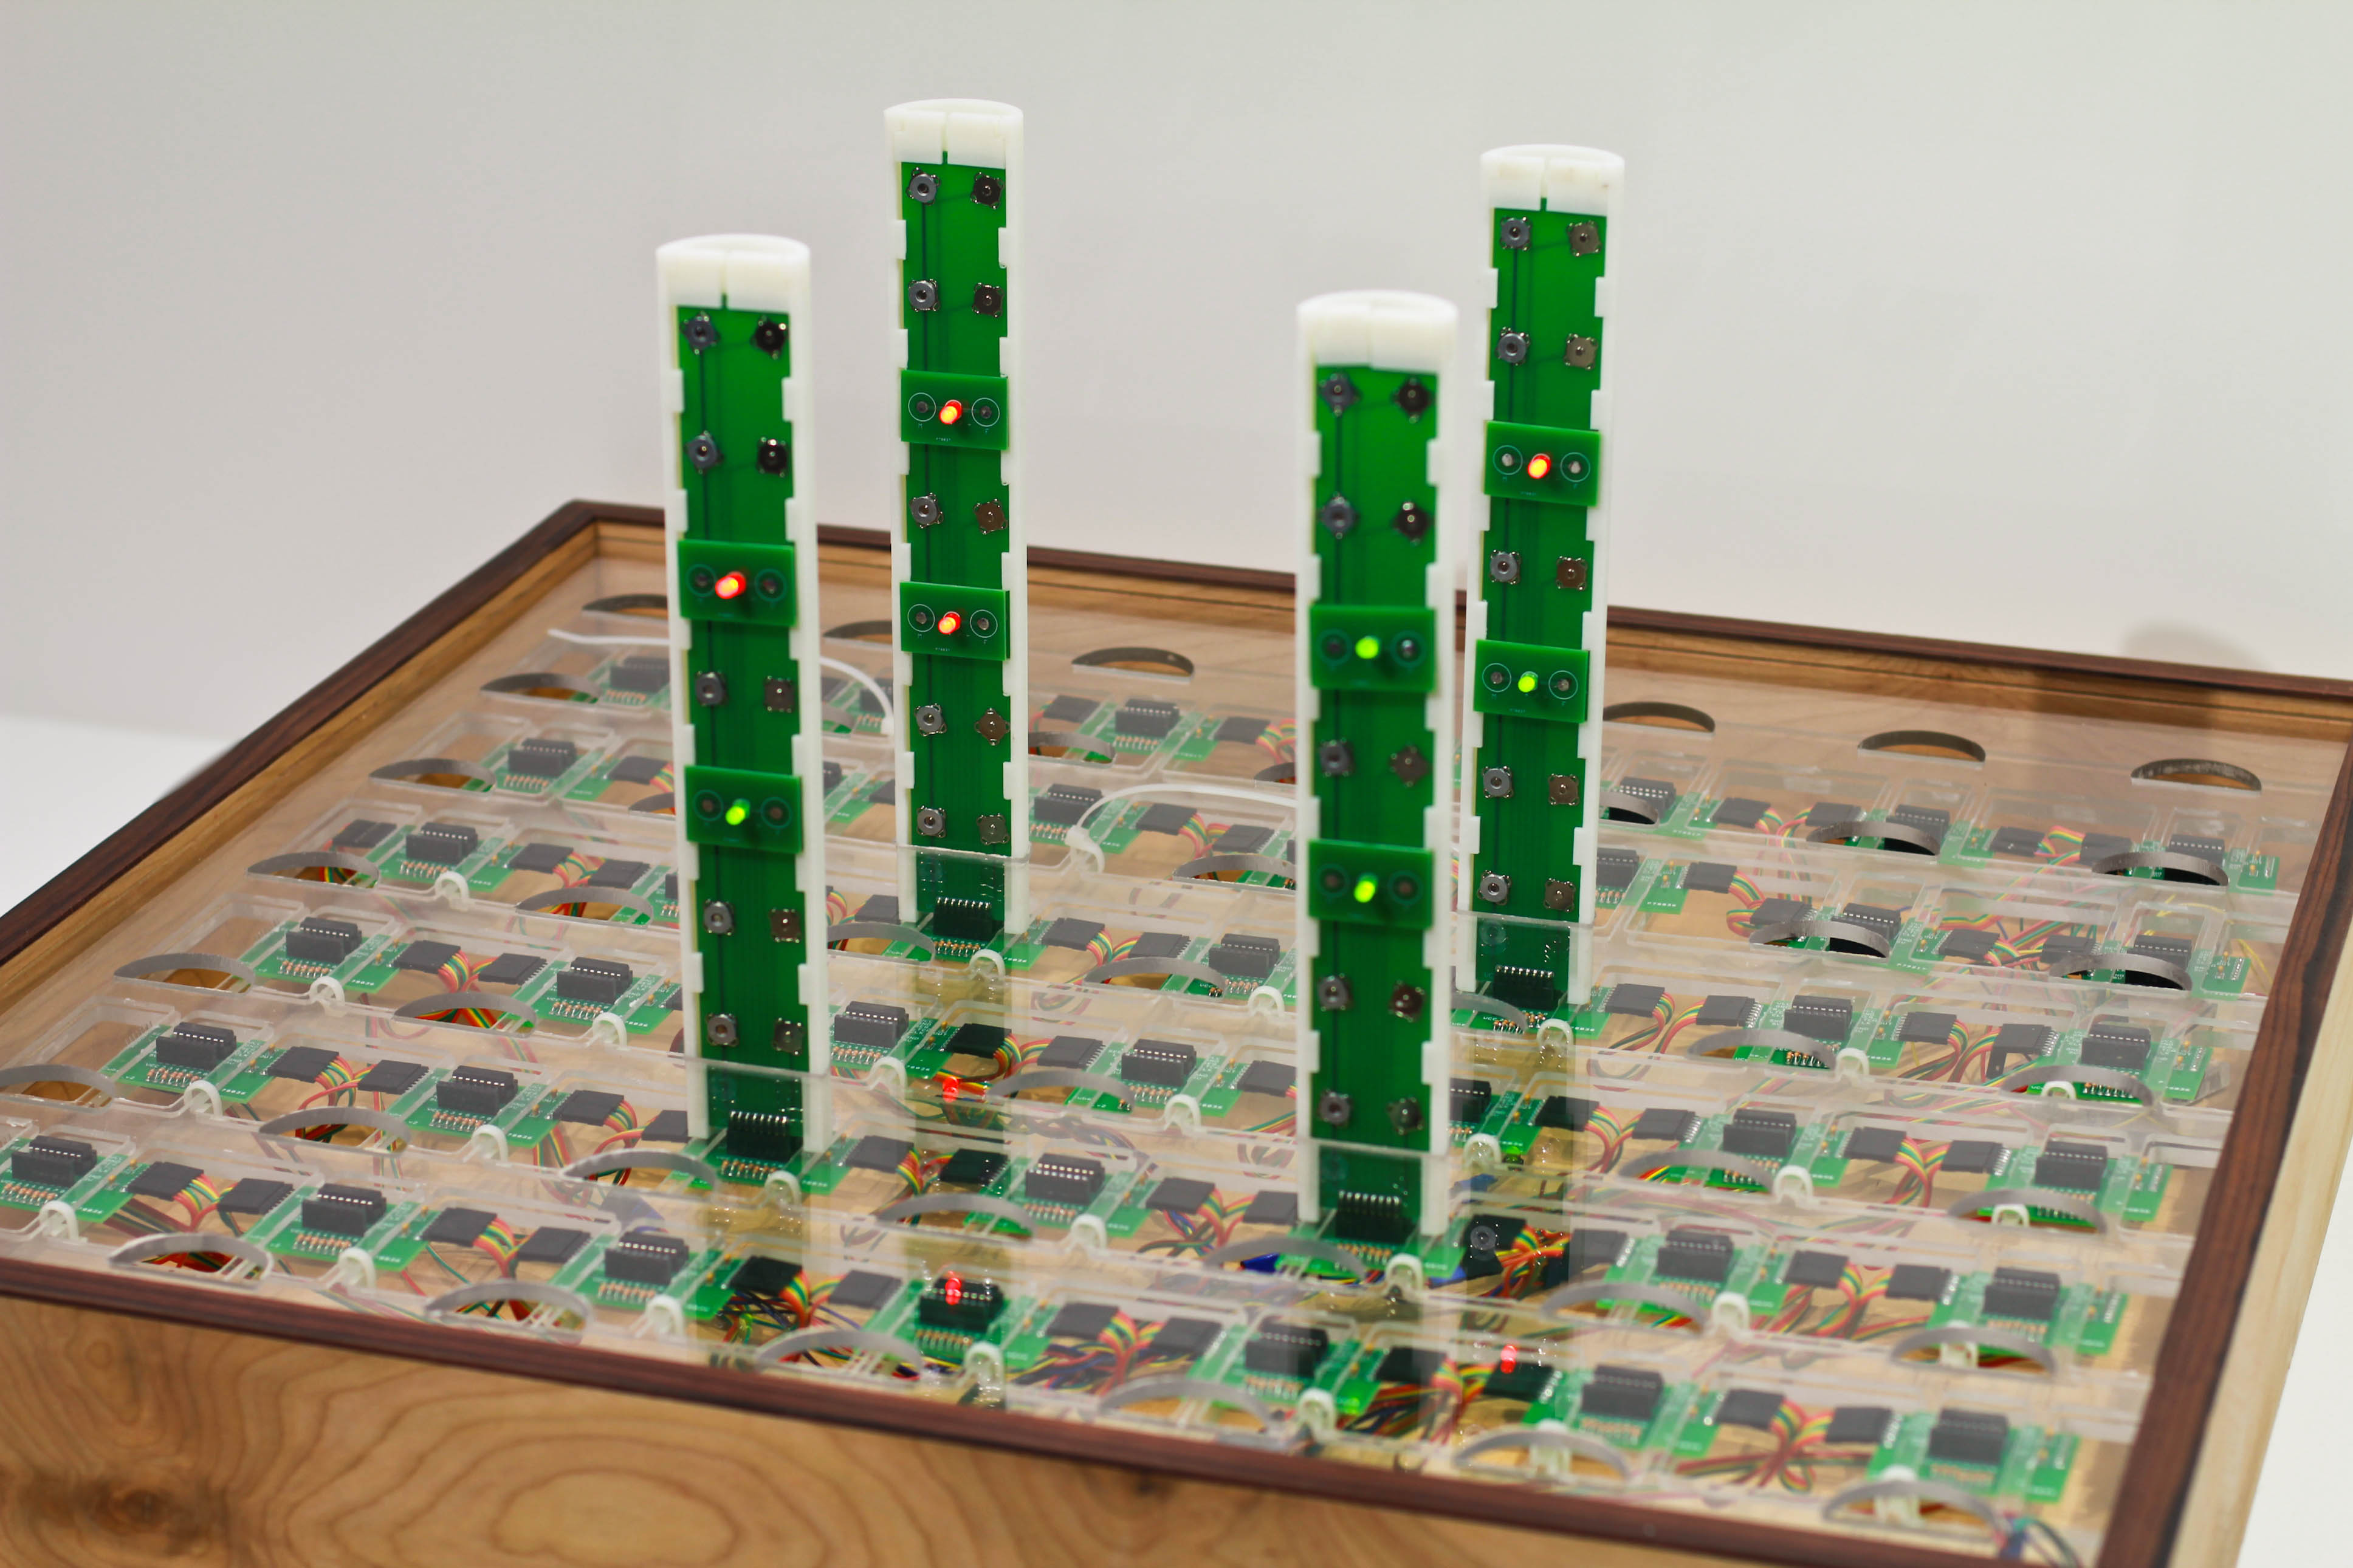
\includegraphics[width=.45\linewidth]{images/BeatriceFinal-2}&
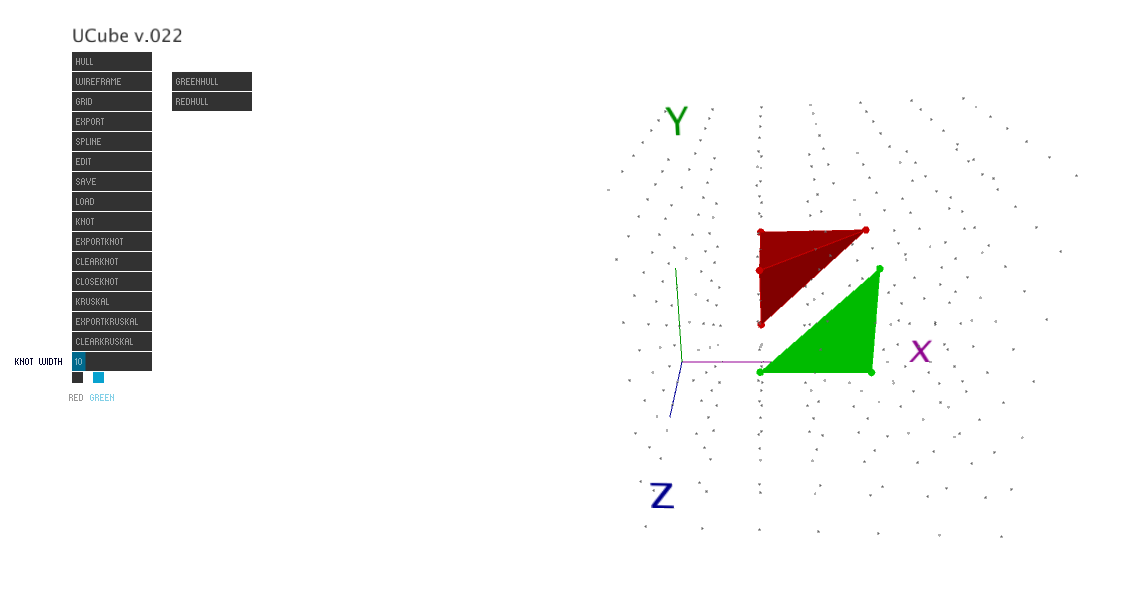
\includegraphics[width=.45\linewidth]{images/twoHulls} 
\end{array}$
\end{center}
\caption{Left: The SnapCAD software showing two convex hulls of different
colors. Right: the SnapCAD software showing a minimal spanning tree model.}
\label{fig:snap2}
\end{figure}


A note on the $7^3$ array in SnapCAD: in our user studies with UCube, we noticed
that users often encountered initial difficulties when required to ``find a
middle'' in the shape they were attempting to model, given an even number of
total grid spaces. For example, to model a pyramid on on a 4x4x4 grid, one needs
to construct a 3x3 subset of the 4x4 grid, using the middle point within the 3x3
set as the top of the pyramid. This influenced our decision to create an
odd-numbered layout, creating a more ``natural'' middle point in the hardware.




\subsection{A Sample (Red/Green Player) Strategy Game for SnapCAD}

In this use case, we make use of the two-color capability of the SnapCAD to
suggest a hypothetical game, or genre of game, that could be created with the
system. The imagined game in question is a geometric strategy game between two
players, ``Red'' and ``Green''. At the outset of the game, each player is given
four lights of her own color; the two of them are told to place their lights at
the eight corners of a cube in the positions shown in the photograph shown in
Figure \ref{fig:snap3} on the upper right.

\begin{figure}[!ht] \begin{center}$
\begin{array}{cc}
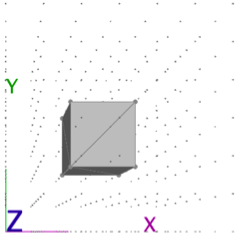
\includegraphics[width=.4\linewidth, height=2.2in]{images/snap_game1}&
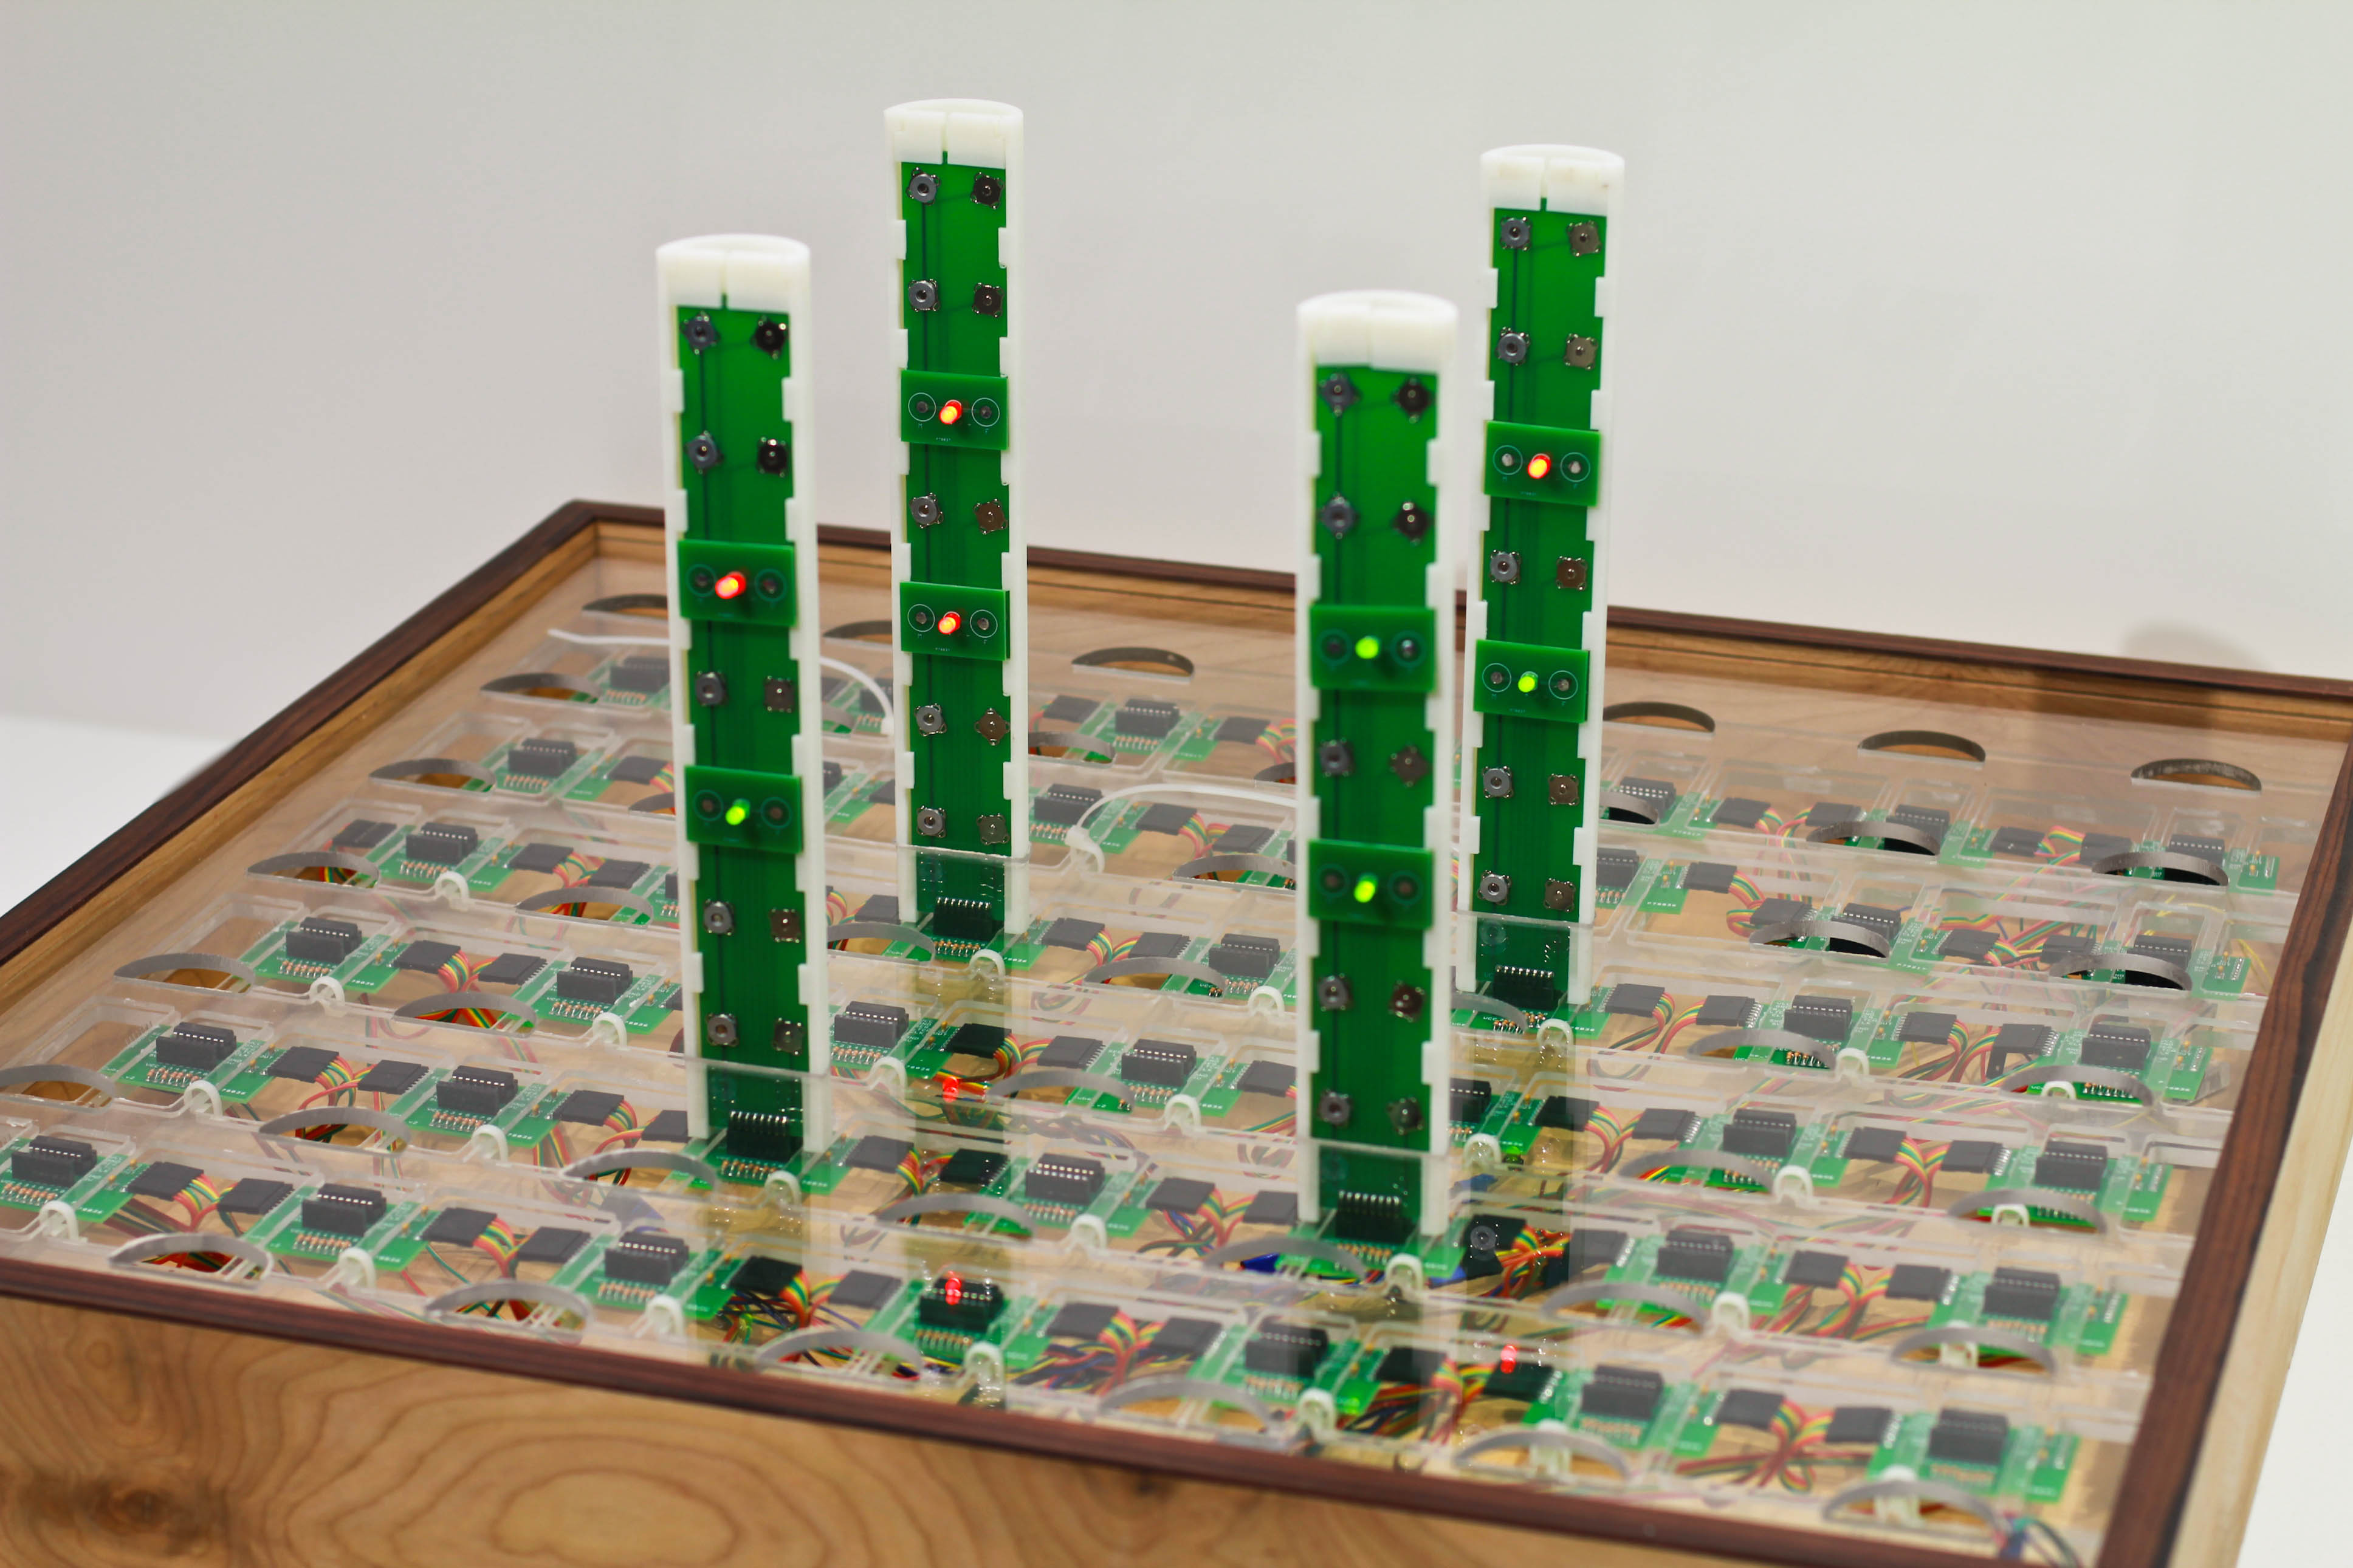
\includegraphics[width=.5\linewidth]{images/BeatriceFinal-2} \\
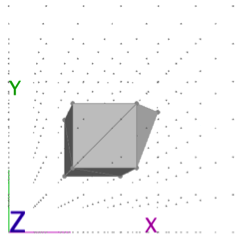
\includegraphics[width=.4\linewidth, height=2.2in]{images/snap_game2}&
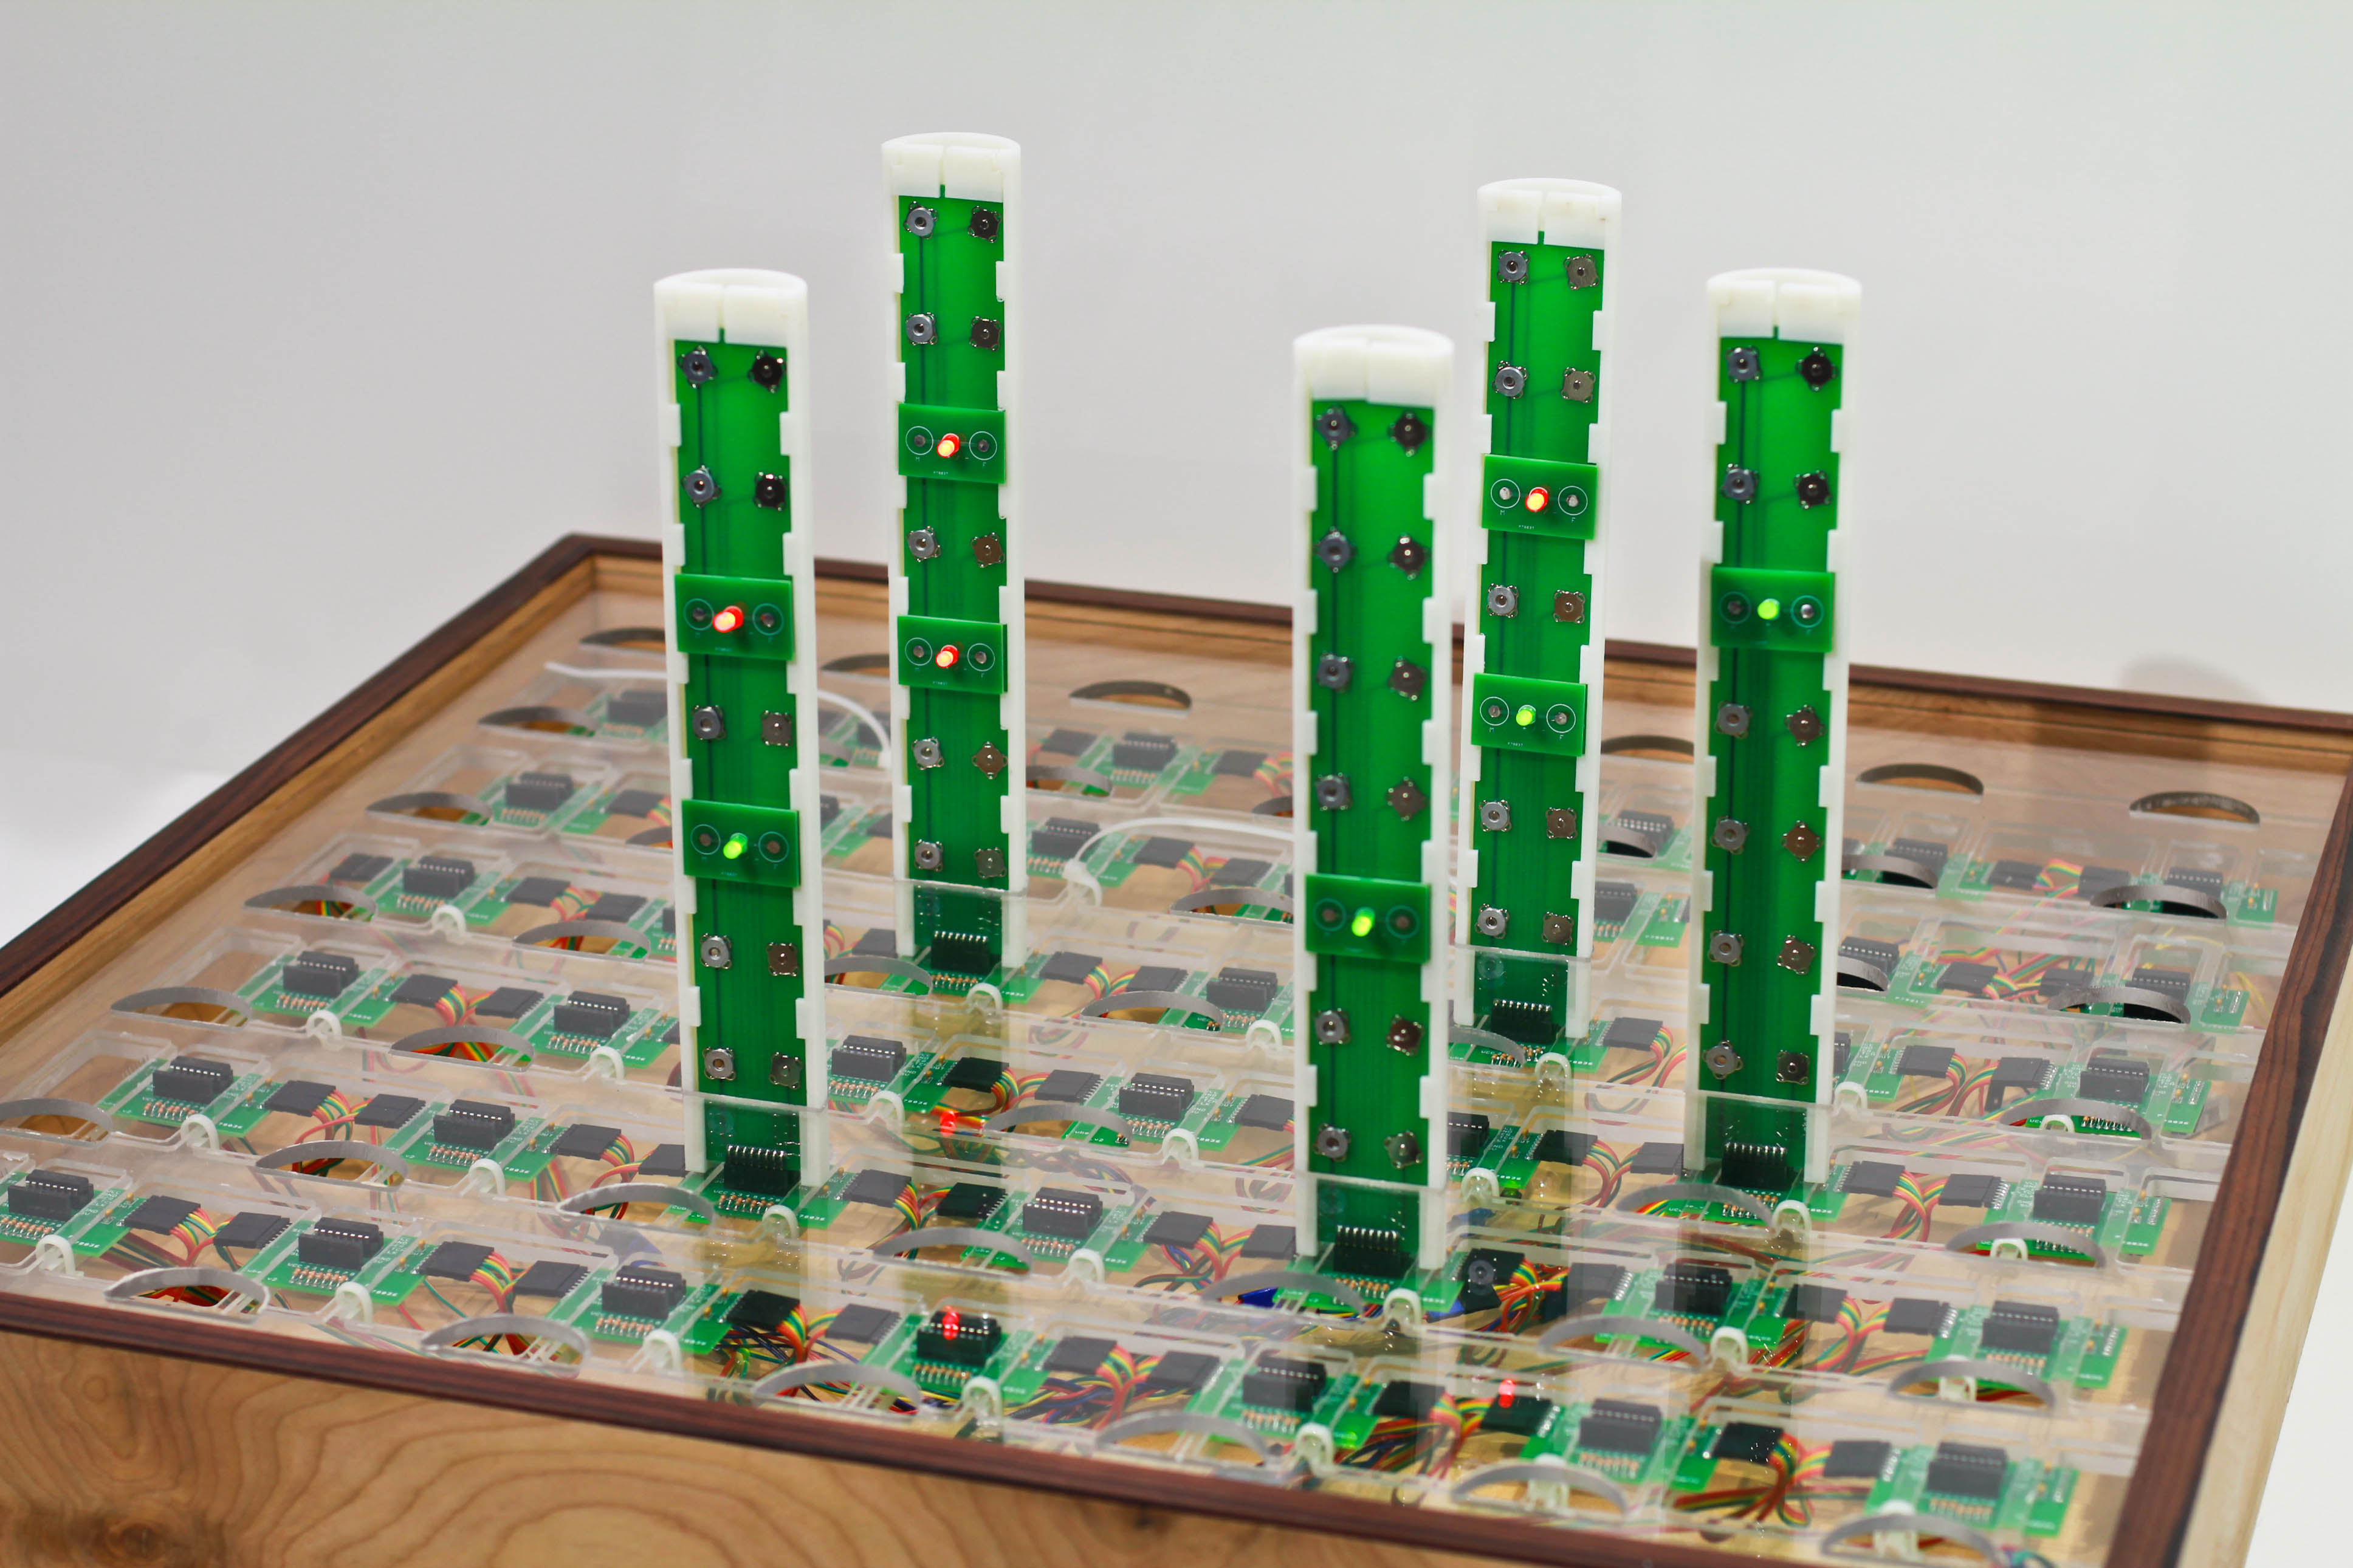
\includegraphics[width=.5\linewidth]{images/BeatriceFinal-3}
\end{array}$
\end{center}
\caption{Left: The SnapCAD software showing two convex hulls of different
colors. Right: the SnapCAD software showing a minimal spanning tree model.}
\label{fig:snap3}
\end{figure}

Now, the computer could display the convex hull of the present set of lights (a
cube), as shown in Figure \ref{fig:snap3} on the upper left; and then (in our
scenario) the computer tells the Green player to move one of her lights to
create the new convex hull shown at the bottom-left of Figure \ref{fig:snap3}.
Thus, the Green player's job is to change the ``cube'' hull to the new hull with
one move of one green light. A correct answer to this challenge is shown in the
photograph of Figure \ref{fig:snap3} at the bottom-right; and if the Green
player makes this correct move, the Red player is now given the (current) convex hull
and yet another hull that could be created with one move of a red light. In this
fashion, the two players take turns moving lights of their own color to produce
a new overall configuration of lights at every step, until one player fails to
solve the current challenge, at which point the game is over.
There are, of course, many variants or extensions of this game that could be
imagined (for instance, a player might be asked to shift two lights, or to add a
new additional light in her color, to create a new convex hull). The purpose of
this example is simply to show that, with the inclusion of two available colors
for spatial points with SnapCAD, a sizable potential landscape of geometric
activities and puzzles becomes feasible.



% \section{Proposed Work: Technical Additions}
% The proposed work is in two sections: technical additions and
% evaluation. This section deals with the technical additions to the proposed
% devices: SnapCAD and PopCAD.
% 
% \subsection{SnapCAD}
% 
% With 343 potential points, a click-and-drag editing tool, and three separate
% modeling modes (convex hull, knot/path, and minimal spanning tree) the SnapCAD
% is capable of generating countless 3-dimensional forms.
% Although the potential for additional modeling tools is certainly a possibility
% (we have yet to experiment with curved surfaces, for instance) we believe that
% the multi-player `platform' aspects of the SnapCAD system are the most ripe for
% development. We already have two colors of LED boards, the ability to display
% two colors of convex hulls, and a 3D implementation of a two-player tic-tac-toe
% game. Displaying multiple colors of the path/knot and minimal spanning tree
% modes should be fairly straightforward to implement.
% We would also like to expand and change the colors currently being used - we
% currently use red and green LEDs, which would be problematic for anyone with
% red/green color blindness. We propose using three colors: red, blue, and purple.
% This not only allows for up to three-player interactions, but could help to
% solve a deeper problem: representing in hardware a node occupied by two players.
% Using an idiom where solely-occupied nodes are either blue or red, and a jointly
% occupied node is purple, we can then expand the types of games, puzzles, or
% modeling activities the SnapCAD system can support. Once these improvements are
% made we can expand the activities supported on SnapCAD. Developments include
% two-to-three player games like tic-tac-toe as well as games built
% off of the modeling capabilities of the SnapCAD (e.g. match the model generated
% by the computer, model a sequential path through a generated maze, place points
% on or interior to the convex hull until there are no more to be found). Colors
% can also be used for certain as-yet unexplored modeling operations (e.g., the
% set union, intersection, or difference). While some of these operations may
% prove difficult or even impossible, these are all avenues worth exploring, as
% they all point towards the extensibility and potential expressiveness of SnapCAD
% as a platform for future development.

\section{PopCAD}

Our motivations for creating a third, alternative interface to the UCube and
SnapCAD stem from the desire to explore this intellectual space more generally;
it is far more interesting to discuss a \emph{class} of tangible interfaces for
scaffolding digital fabrication than it is to discuss a singular device. To this
end, we looked at some of the weaknesses of SnapCAD and towards technologies we
had yet to explore. While SnapCAD can admirably perform a number of modeling
tasks, it was always envisioned as one device amongst an ``ecosystem'' of next
generation fabrication tools. It has strengths, but obvious weaknesses as well;
in particular, the SnapCAD hardware was expensive to produce, and so would be a
difficult proposition for some schools or fab labs to produce or purchase; it is
also rather unwieldy and unportable - it is moderately heavy, fairly large (over
30 inches square), and has many separate pieces (like the towers and LED boards)
that could break or go missing. Thus, an interface with cheaper and more
portable materials was desirable.

To address these issues we chose to build a pop-up book combining traditional
paper-crafts and paper-friendly electronic components such as copper or
conductive tape and conductive inks.
In recent years, revolutionary work has been done in combining electronics and
paper
crafting\cite{Qi:2010:EPE:1709886.1709909}\cite{Mellis:2013:MMC:2460625.2460638},
leading to new techniques and new uses for traditional materials. Paper is
inexpensive (especially when compared to circuit boards), light, and easily
portable, making it an ideal material choice for a device that would not suffer
the same limitations present in the SnapCAD. Although we often think of
``paper'' as a rather static material, there are in fact many variations in the
size, weight, color, transparency, and composition of contemporary paper
products. We will cover the two paper-based prototypes we created in this vein,
dubbed ``PopCAD v1'' and ``PopCAD v2''.

\subsection{PopCAD v1}

For the initial prototype, we use a simple construction paper as it provides a
balance between strength and flexibility as well as having a consistency
well-suited to laser etching and cutting. The pop-up book (named PopCAD) has a
3x3x3 array of 27 points which are evenly spaced three inches apart on a 12'' x
18'' paper surface. The book folds on a single center crease making the closed
footprint of the book roughly 12'' x 9''.

\begin{figure}[!ht] \begin{center}$
\begin{array}{cc}
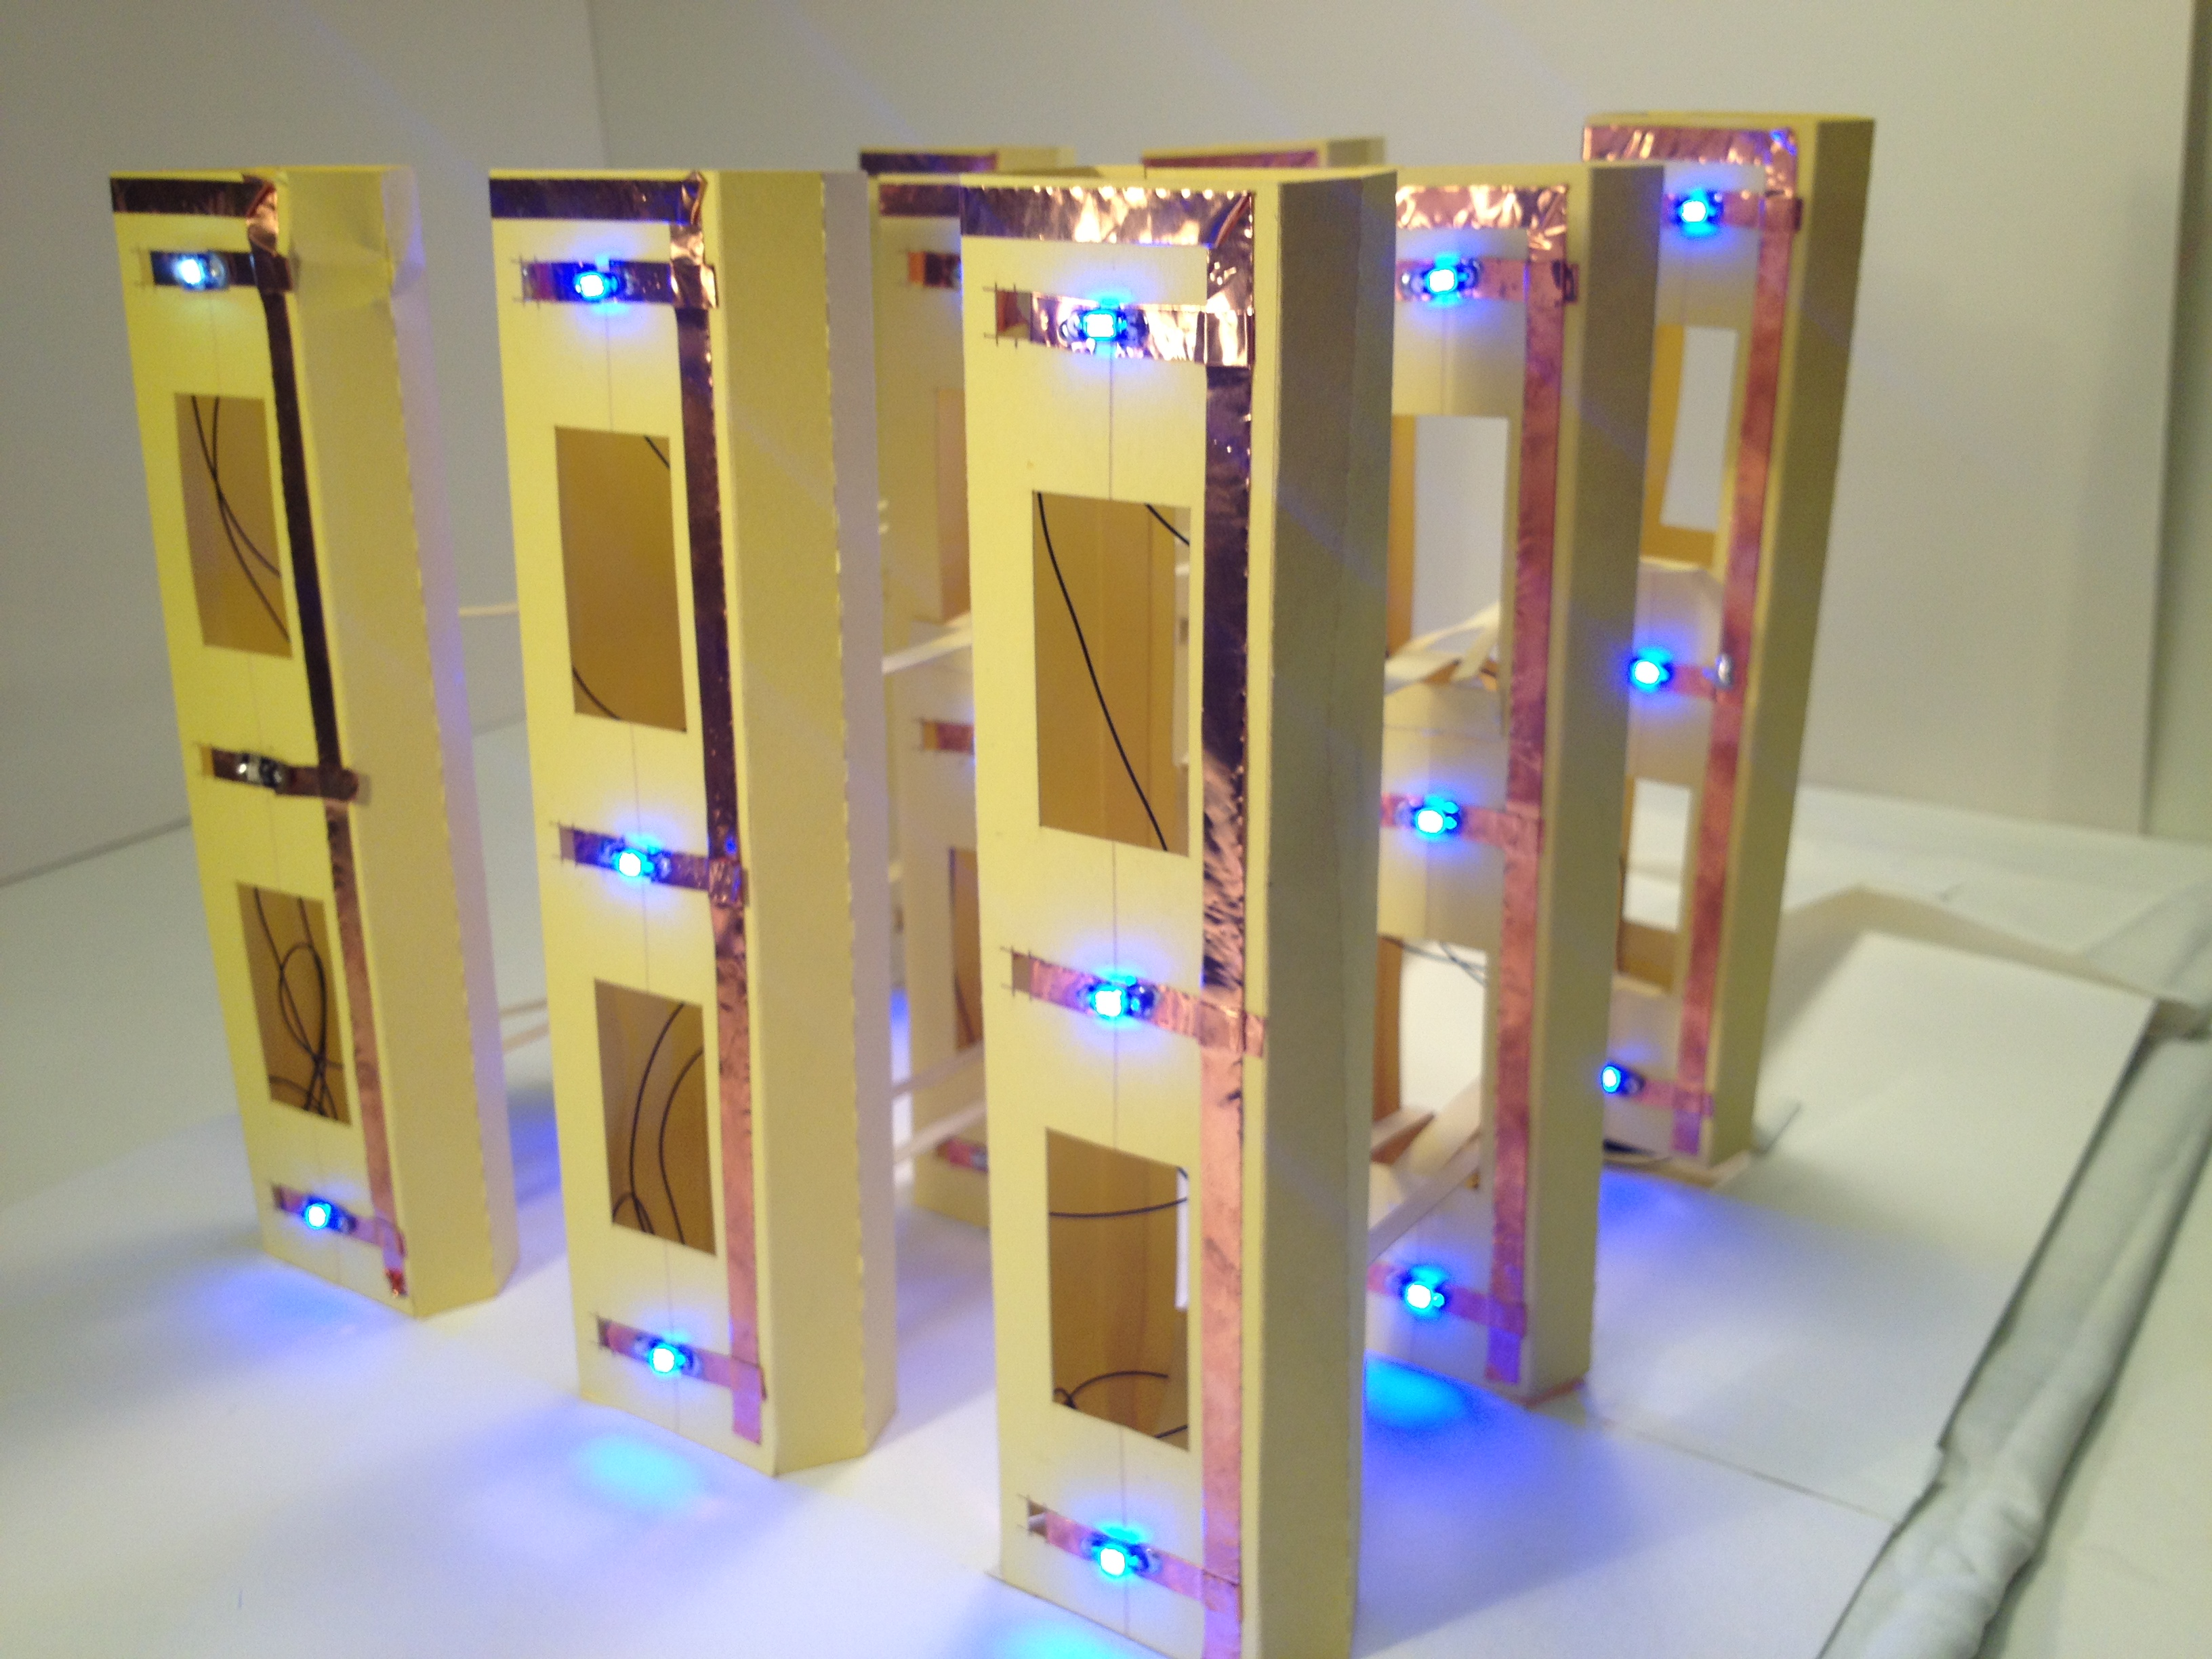
\includegraphics[width=.45\linewidth]{images/popcad25}&
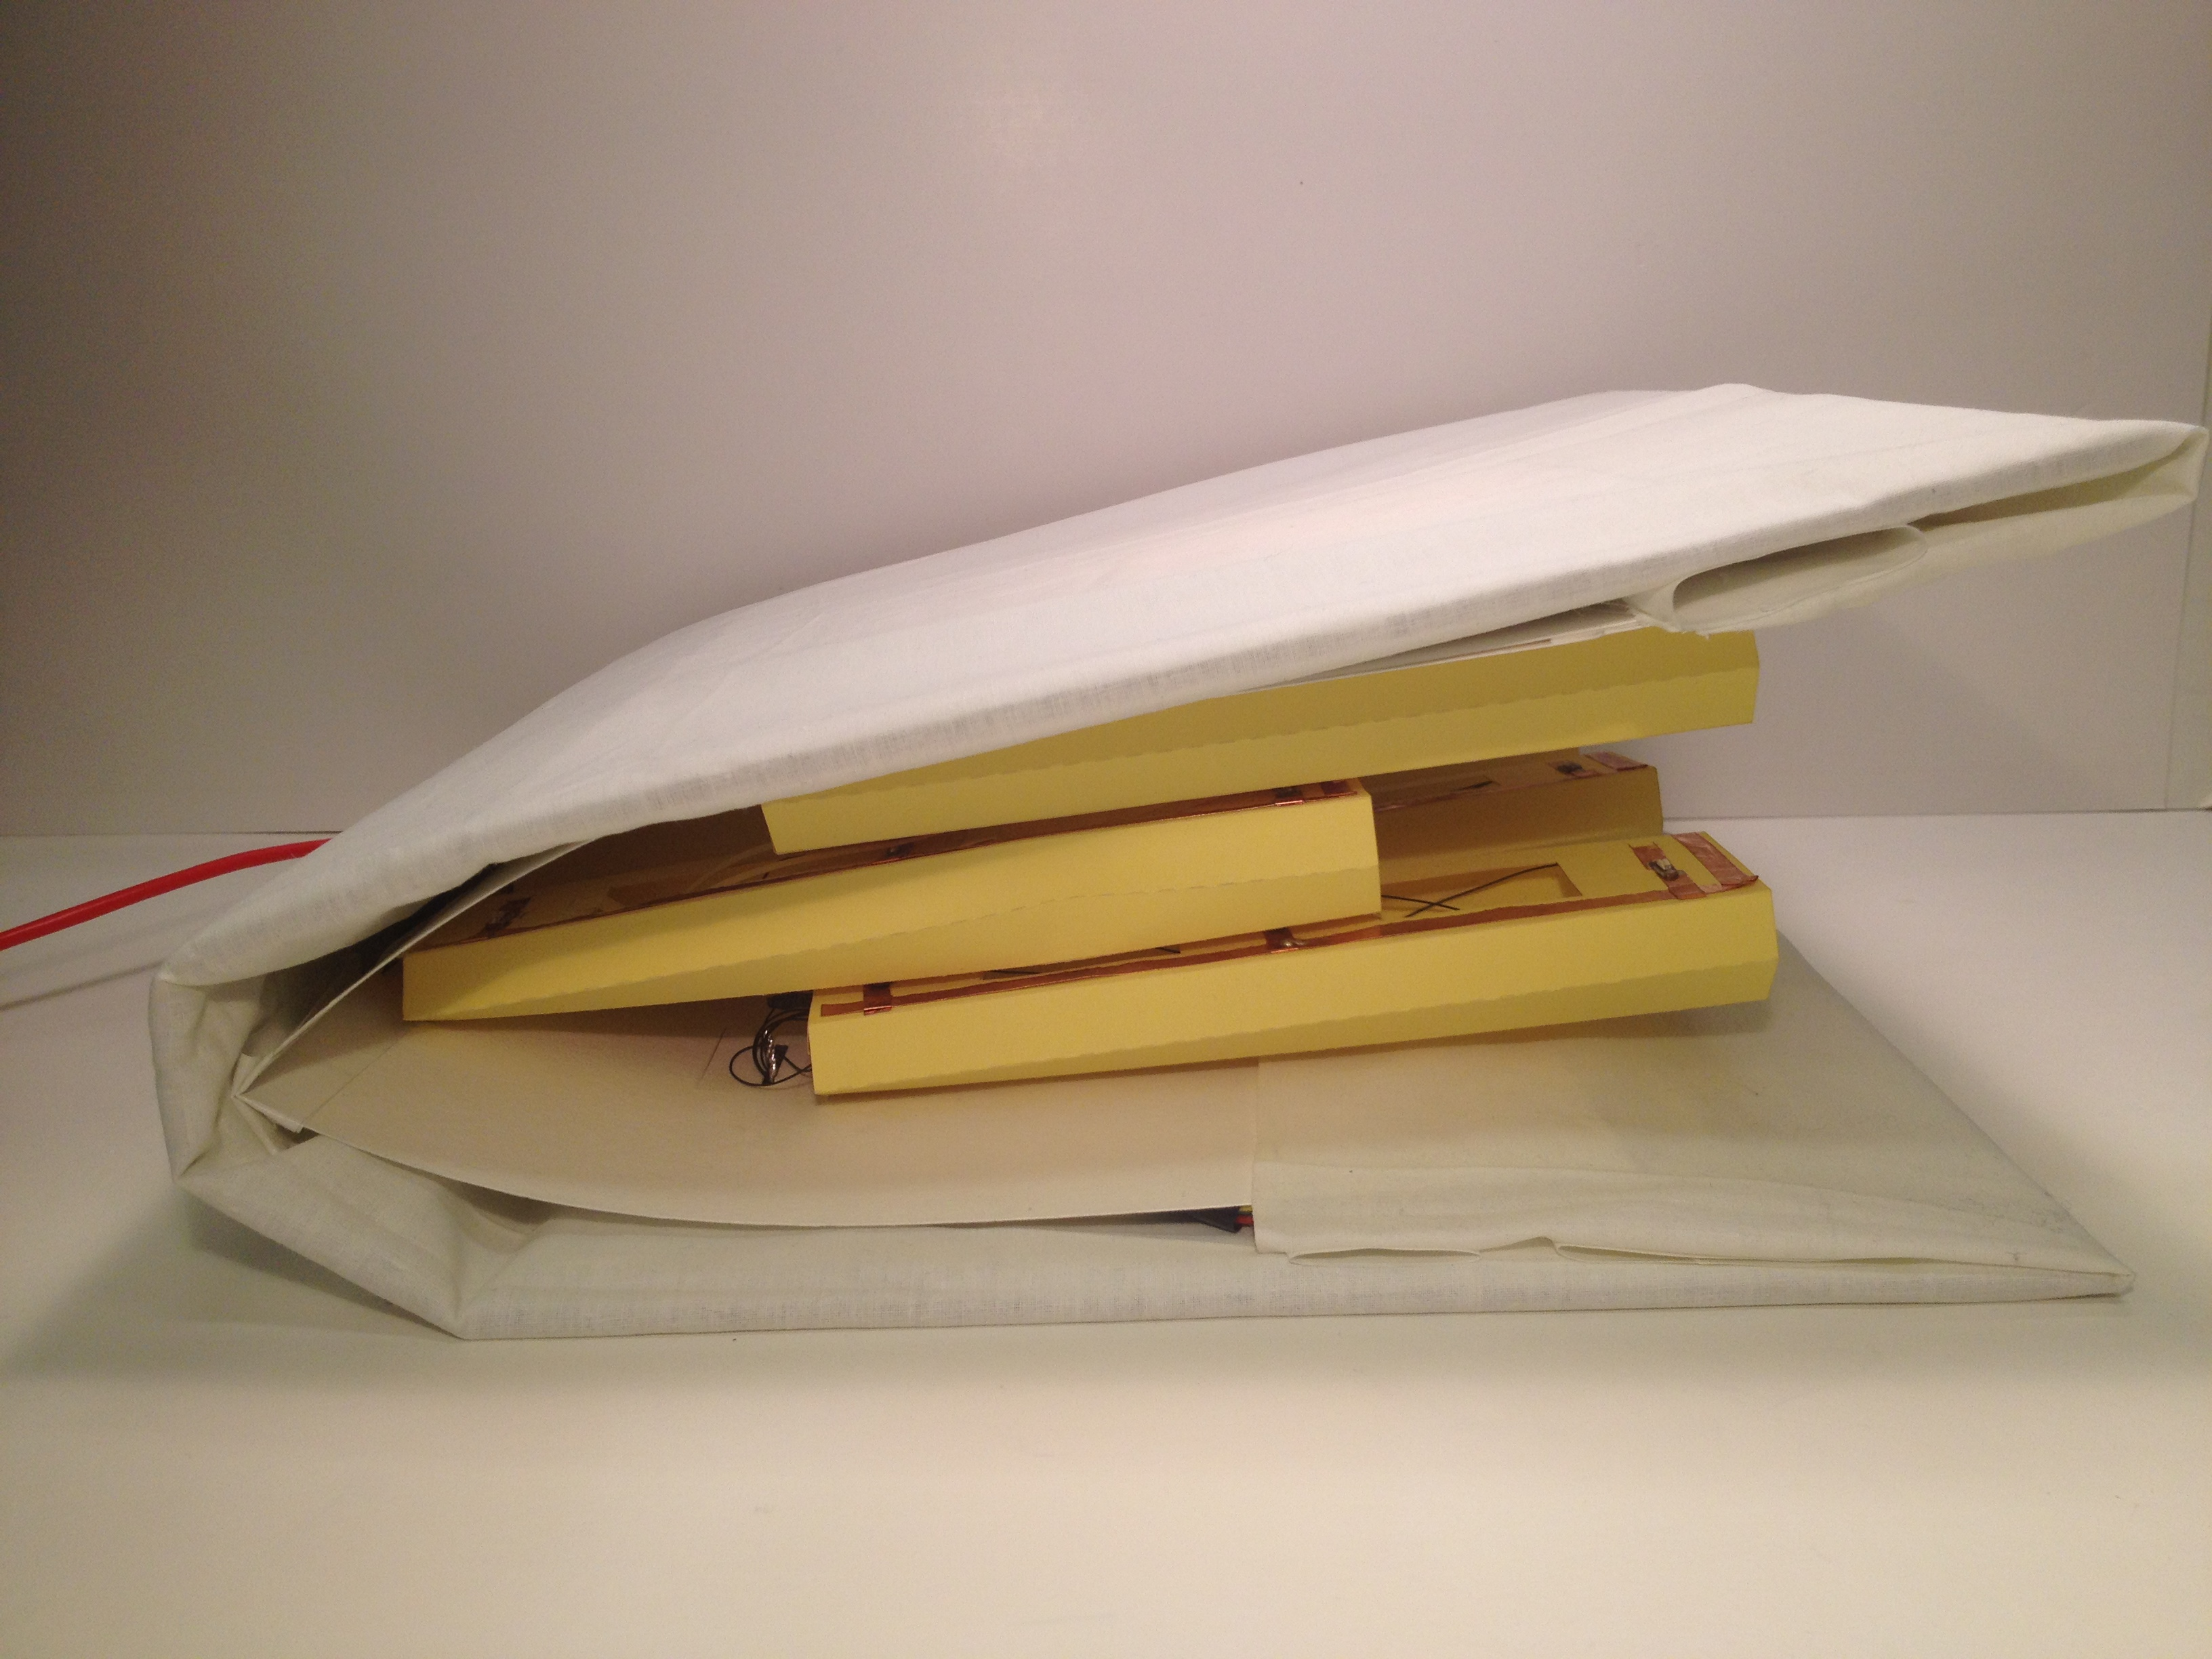
\includegraphics[width=.45\linewidth]{images/popcad44}
\end{array}$
\end{center}
\caption{Two views of the first pop-up book prototype, showing the interface in
both open and closed states.}
\label{fig:popup}
\end{figure}

Each tower has a copper tape circuit consisting of three LEDs on the front face
and three corresponding capacitive touch sensors on the left face. The copper
tape acts as a paper-friendly conductive material to connect the electronic
components together much like traditional wire. The LEDs are soldered onto the
copper tape for greater stability. The capacitive sensors are simply a piece of
copper tape which is connected to a pin on a microcontroller (in the first
version, this is an Arduino Mega Pro). By bringing the internal pull-up resistor
connected to the pin ``LOW'' (to ground) and then timing how long it takes to get
back to a ``HIGH'' state we can tell if the connection is being influenced by a
capacitive force. For example, if there is no interference on the circuit, the
timer will normally only get to ``1'' before the resistor is back to a HIGH state;
if a finger is placed on the copper tape, the reading will be
much higher (typically around ``17''). Based on this change, we can detect which
switch was touched and toggle the associated LED on or off. The hollow interior
of each paper tower is used to solder thin 30-gauge wire to the three LEDs, the
three switches, and ground. These seven wires are soldered to a row of headers
that stick through the bottom of the first layer of the pop-up book. Wires are
then run along the backside of the top layer of paper from these headers to the
microcontroller. The entire circuit in then encased in a cloth-covered cardboard
binder that acts as a book cover as well as a means to protect and hide the
electronics.

\begin{figure}[!ht] \begin{center}$
\begin{array}{cc}
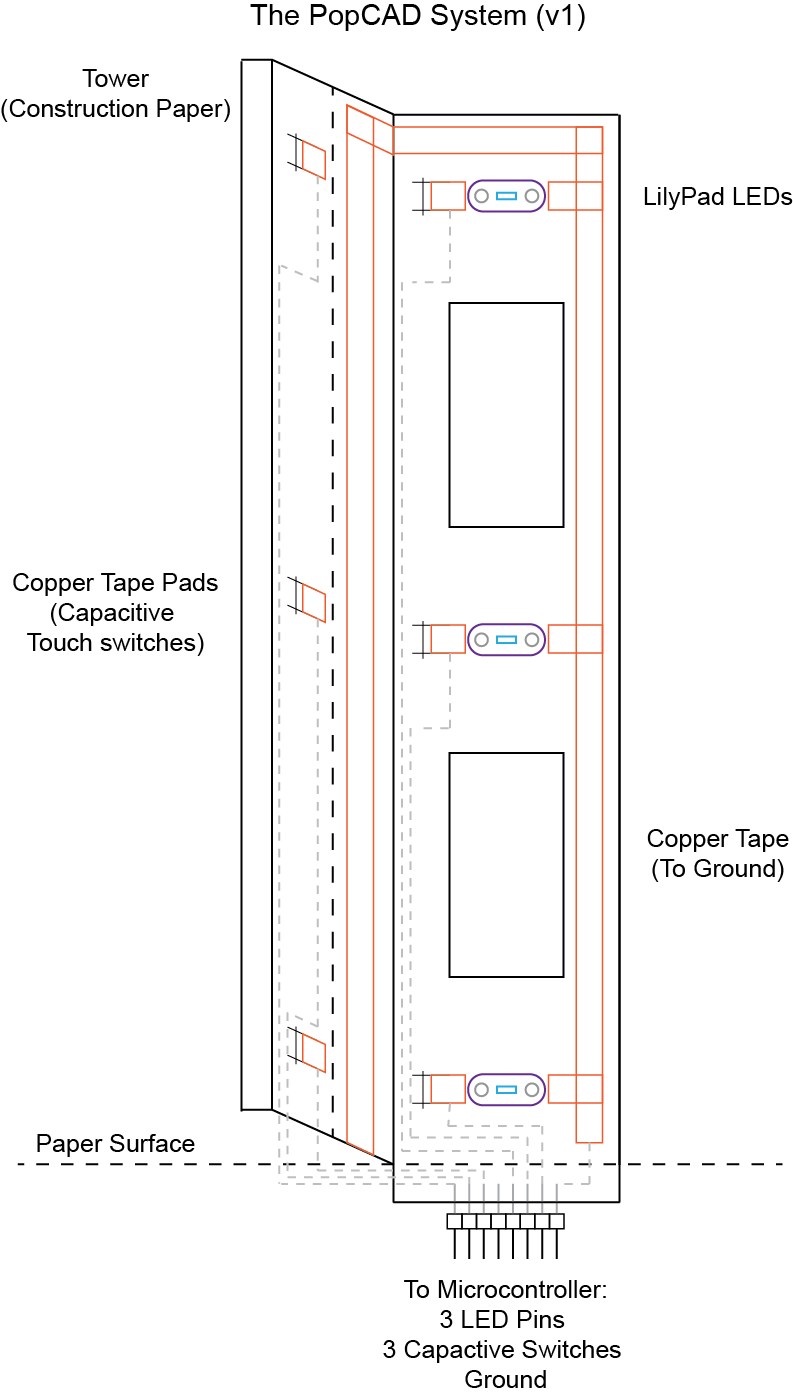
\includegraphics[width=.4\linewidth]{images/PopCadSchematicV1}&
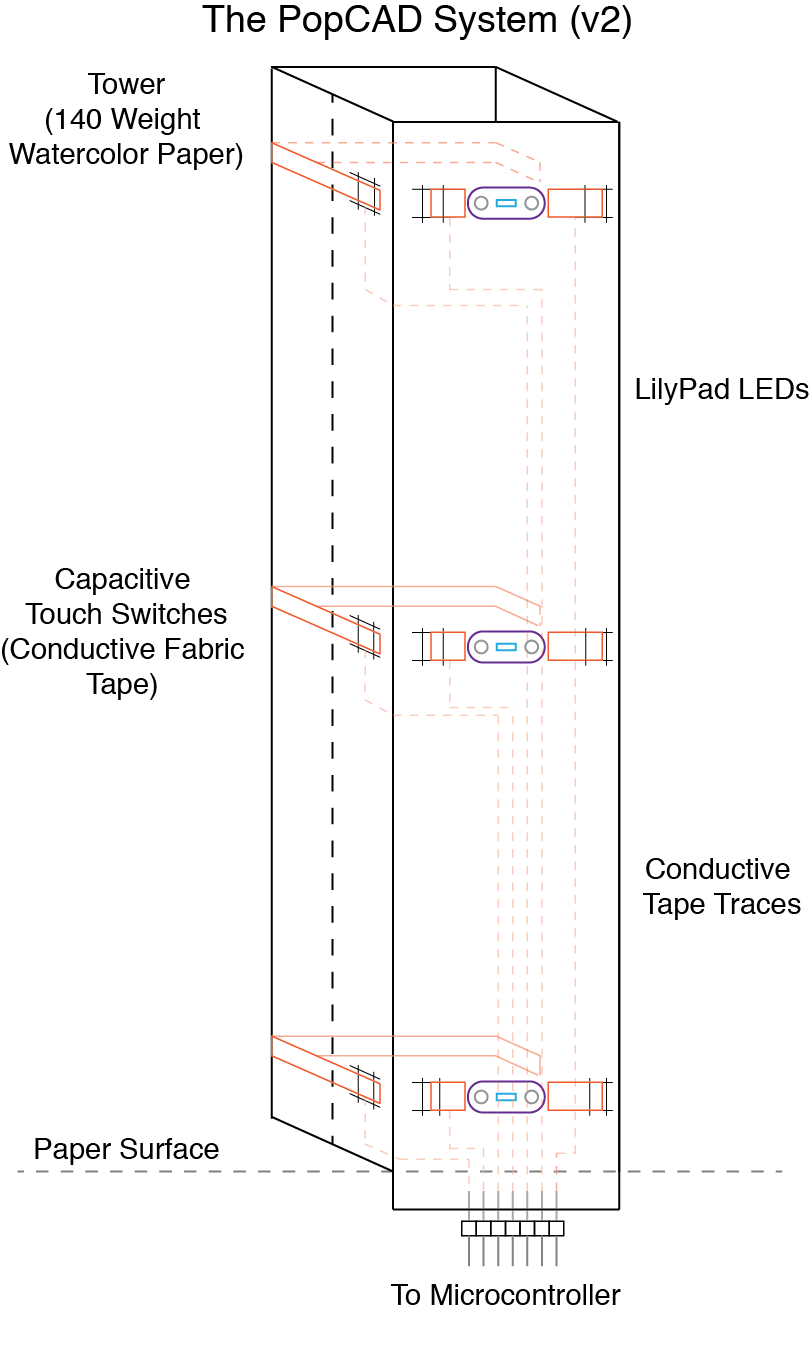
\includegraphics[width=.42\linewidth]{images/PopCadSchematicV2}
\end{array}$
\end{center}
\caption{The two PopCAD designs side-by-side: PopCAD v1 (left) uses copper tape
and 30 gauge wire for the paper circuit, while PopCAD v2 (right) uses
fabric-based conductive tape without needing any wires.}
\label{fig:popup_schematic1}
\end{figure}

\subsection{PopCAD v2}
% 
% This is where we talk about the differences: conductive tape, laser cutting,
% paper choice circuit wiring is more efficient, no horizontal struts\ldots

Although the first PopCAD iteration was a fully-functional prototype, as we
approached user testing with the PopCAD it became apparent that there
were several compelling reasons to iterate on the original design. Through a few
informal user evaluations as well as our own reflections on the device, we
identified several key issues that could be improved upon: (a) the paper
engineering design, (b) the structural integrity of the book as a whole, and (c)
the lack of ``paper-ness'' with respect to the circuitry and electrical
components of the design.

 \begin{figure}[!ht]
  \centering
  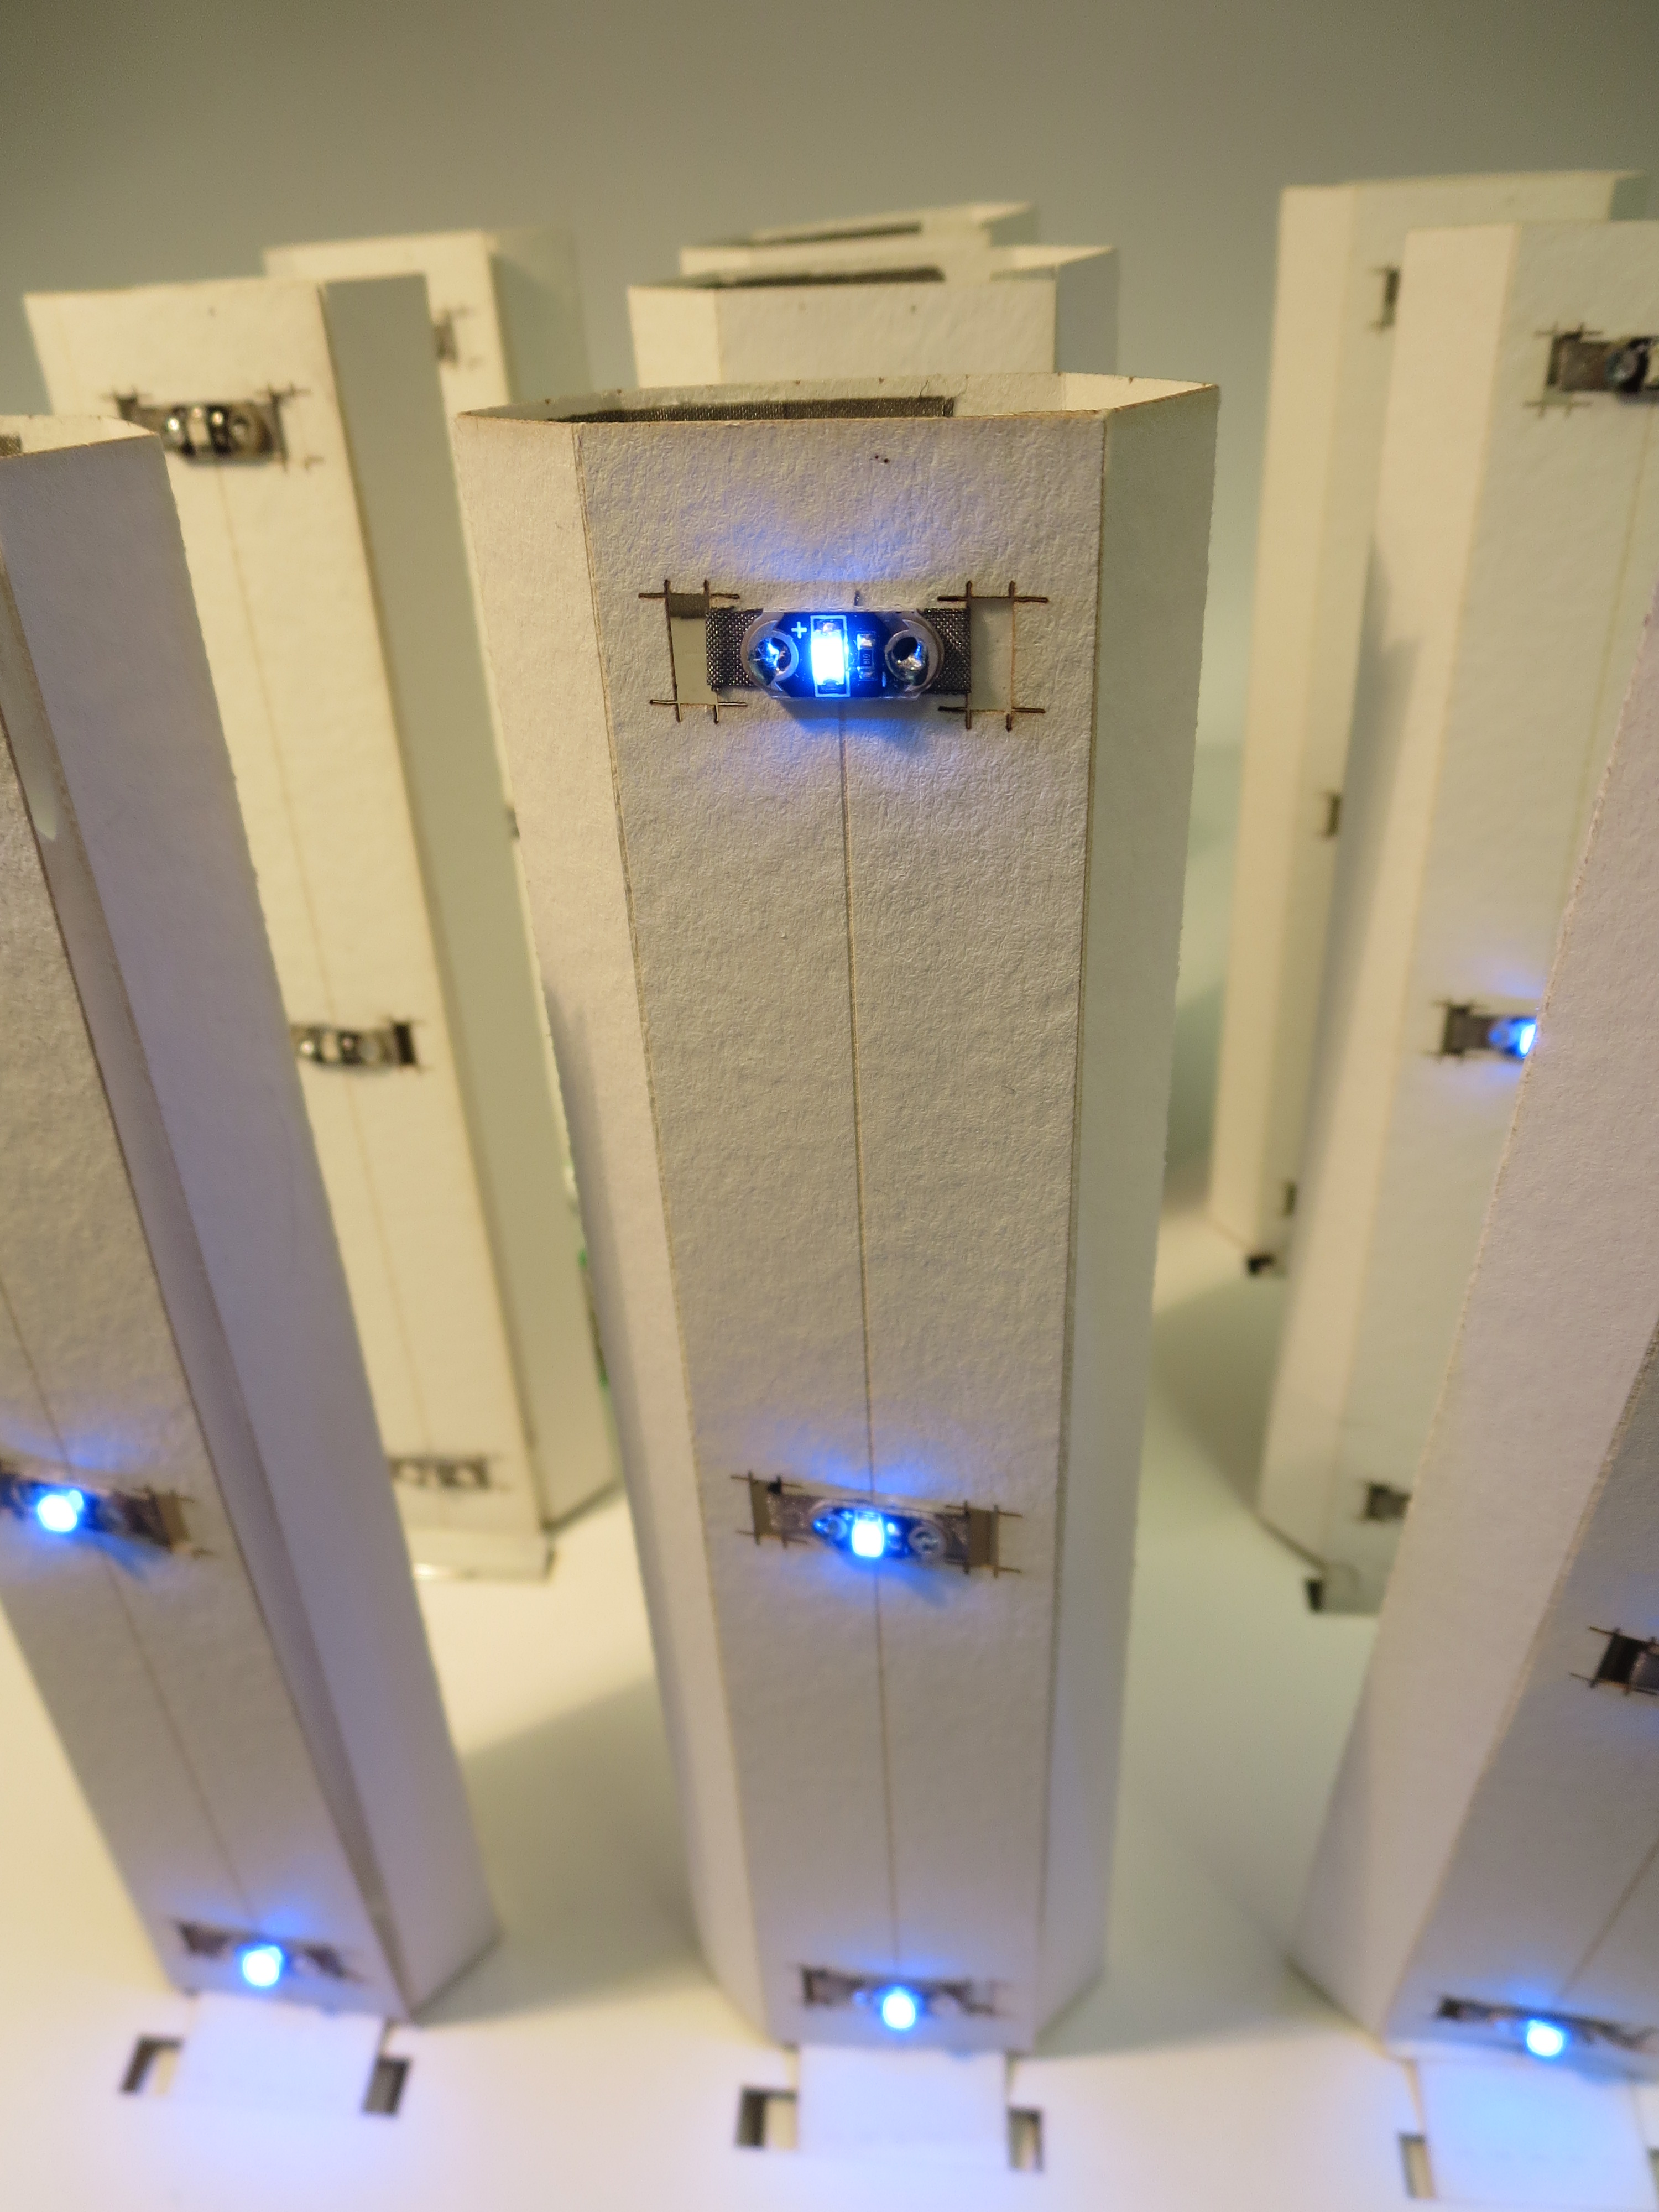
\includegraphics[width=.4\linewidth]{images/pop3}
  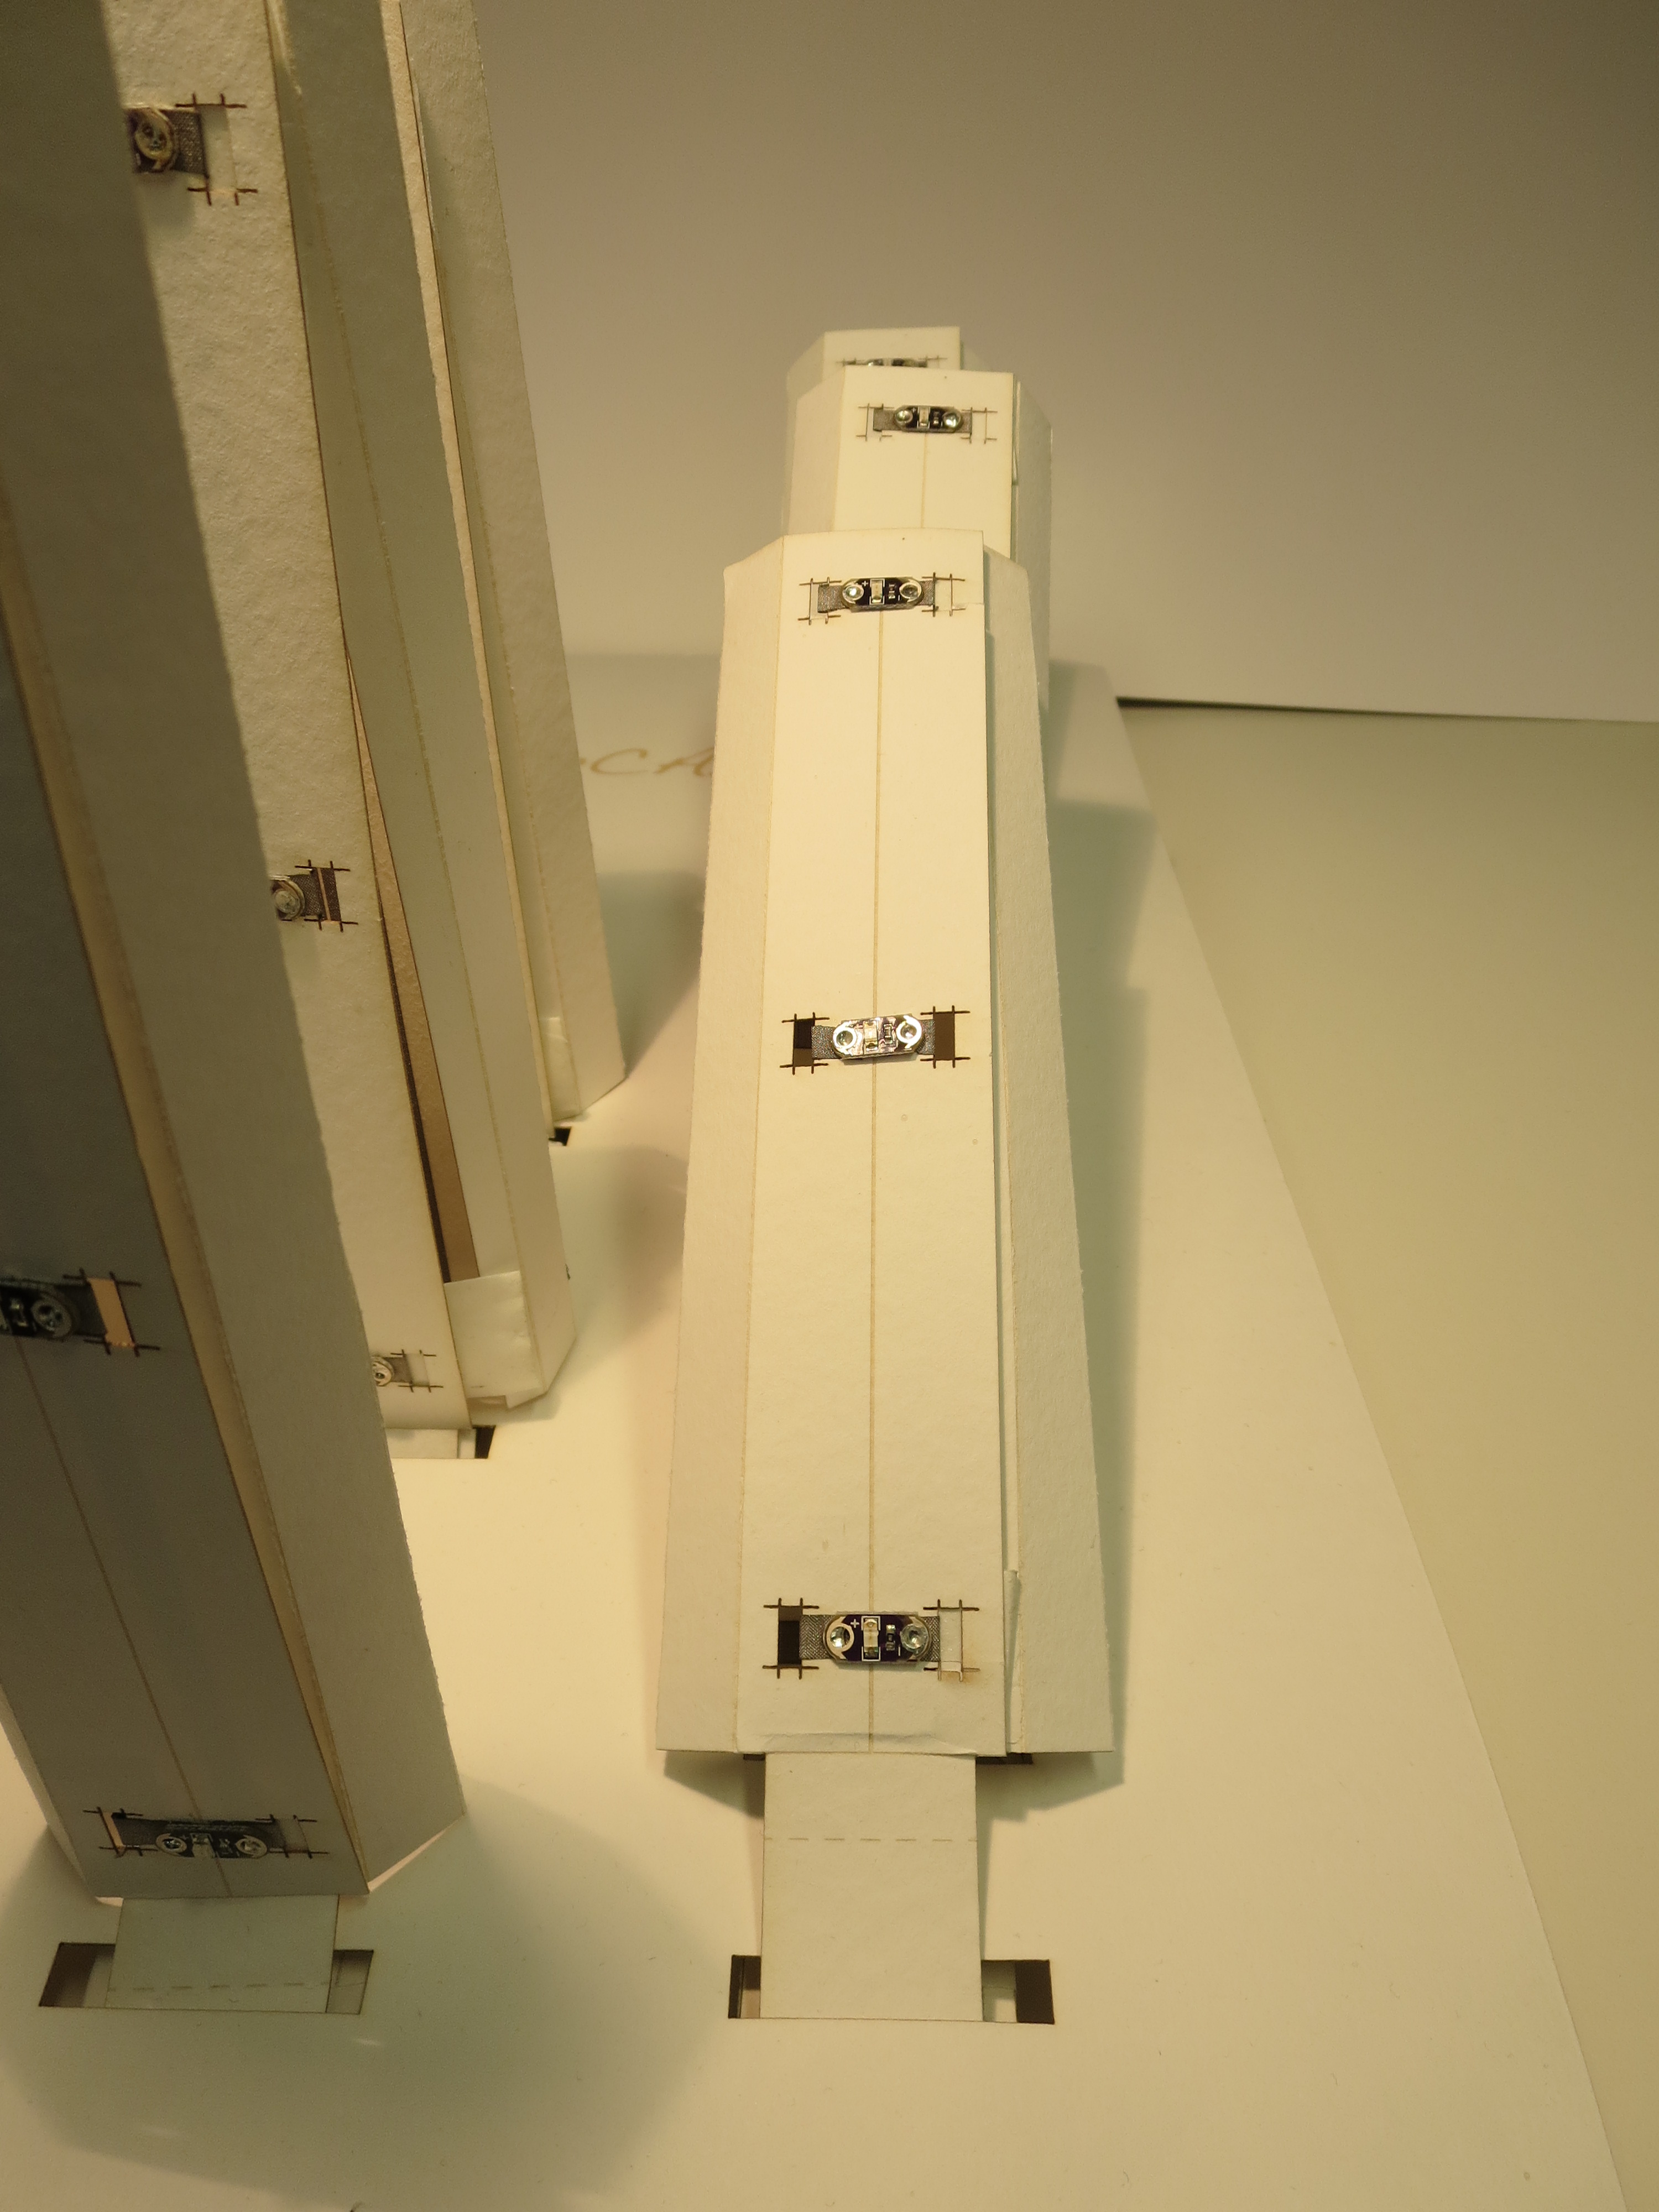
\includegraphics[width=.4\linewidth]{images/popcad_pic2}
  \caption{Two views of PopCADv2 design: with towers raised and LEDs lit
  (left), and with the rightmost column of towers laid flat (right).}
  \label{fig:popcad1}
\end{figure}

To start with the first point above, then: a look at the initial design of the
pop-up mechanism reveals the presence of horizontal paper ``struts'' connecting
the towers in the middle column (along the center crease) to their counterparts
on either side. These struts were necessary in order to generate a pop-up motion
from the middle of a book and force each tower upright. The mechanism was
successful; however, the struts directly interfered with the ability to reach
many of the conductive tape switches. In version two of the PopCAD, the struts
were removed in favor of a pull-tab system whereby each row of towers is raised
and lowered by a tab at the front of the row (the pull tab system can be seen in 
Figure \ref{fig:popcad1}).

We were concerned about the overall stability of the first prototype; lights
would sometimes fail to operate properly, the horizontal struts kept breaking,
parts of the towers were weak, certain points in the wiring were weak, and the
opening and closing of book (and thus the folding of the towers) put enough
strain on the circuitry that we were concerned whether it would survive a user
study. The second prototype addresses these issues in several ways: first, we
use a heavy watercolor paper (140 weight) for all the paper engineering, making
the towers and the pull-tab mechanisms more resilient to repetitive use. Second,
we replace the copper tape, which has a tendency to break over heavy creases,
with conductive fabric tape, which resists repeated creasing much better, and
finally, we made adjustments to lessen the strain on the towers and the
circuitry, by minimizing stress points and reinforcing known weak spots.

\begin{figure}[!ht] 
\begin{center}$
\begin{array}{cc}
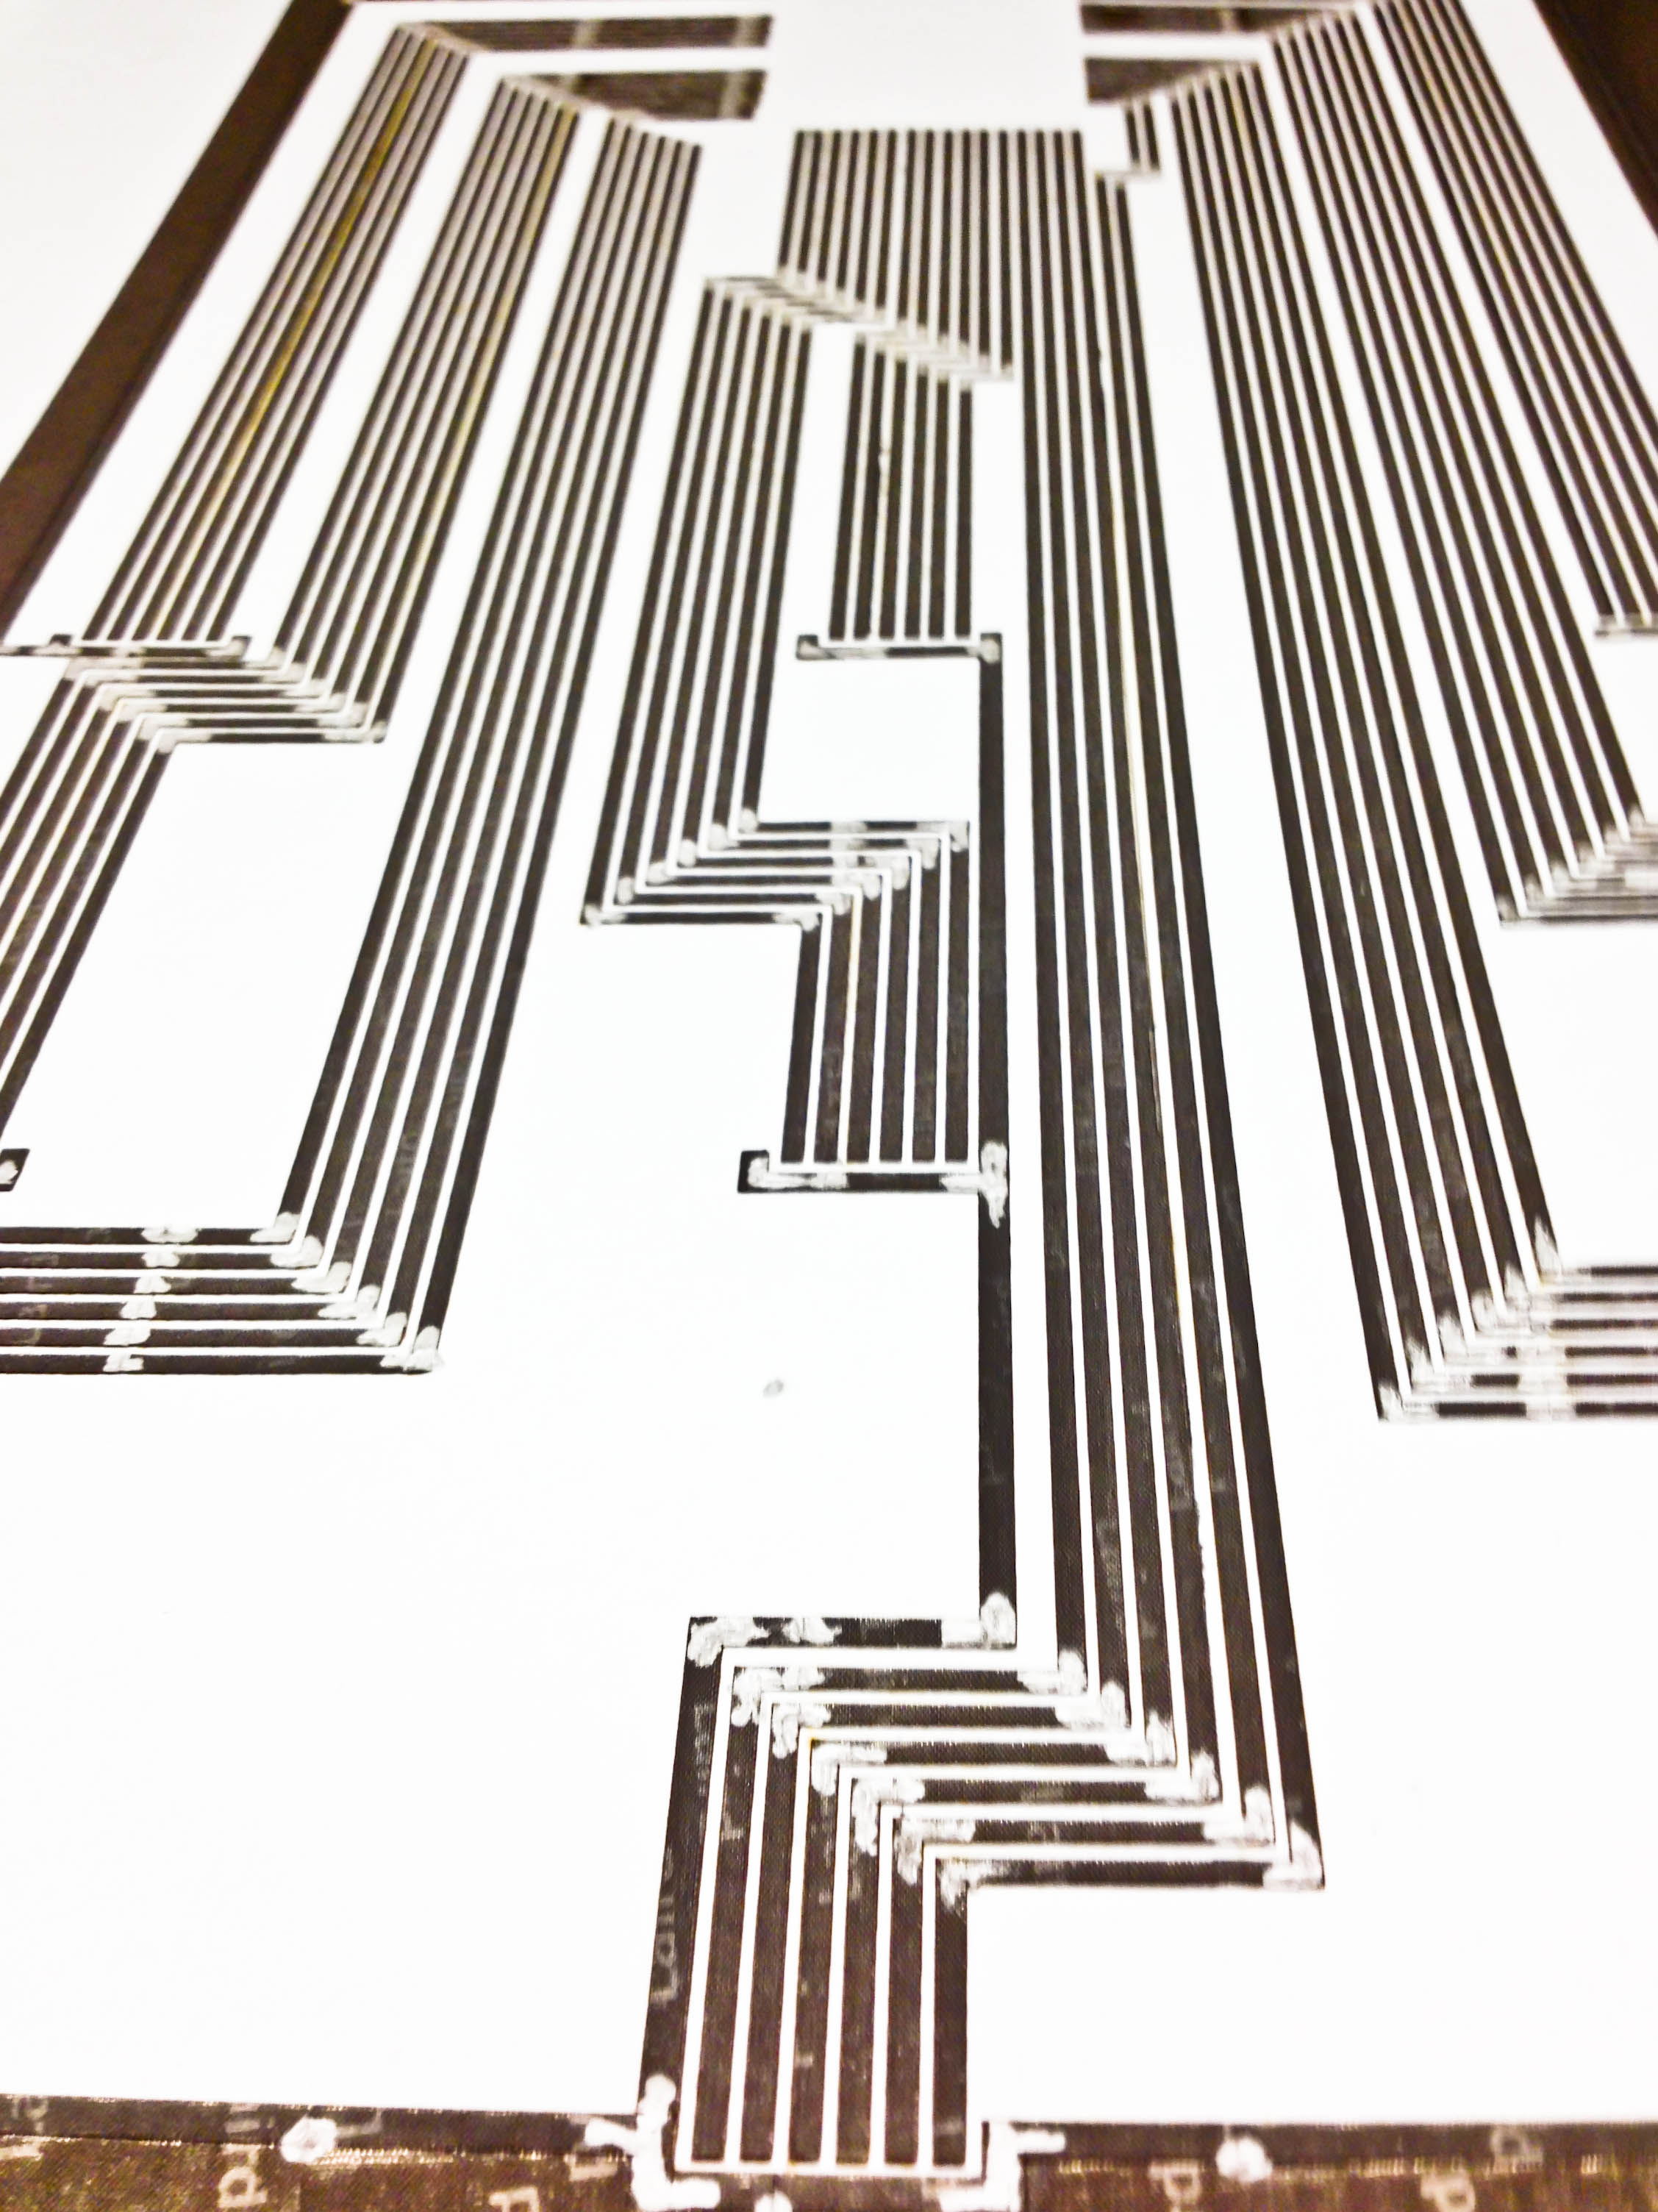
\includegraphics[width=.3\linewidth]{images/pop_circuit2-2}&
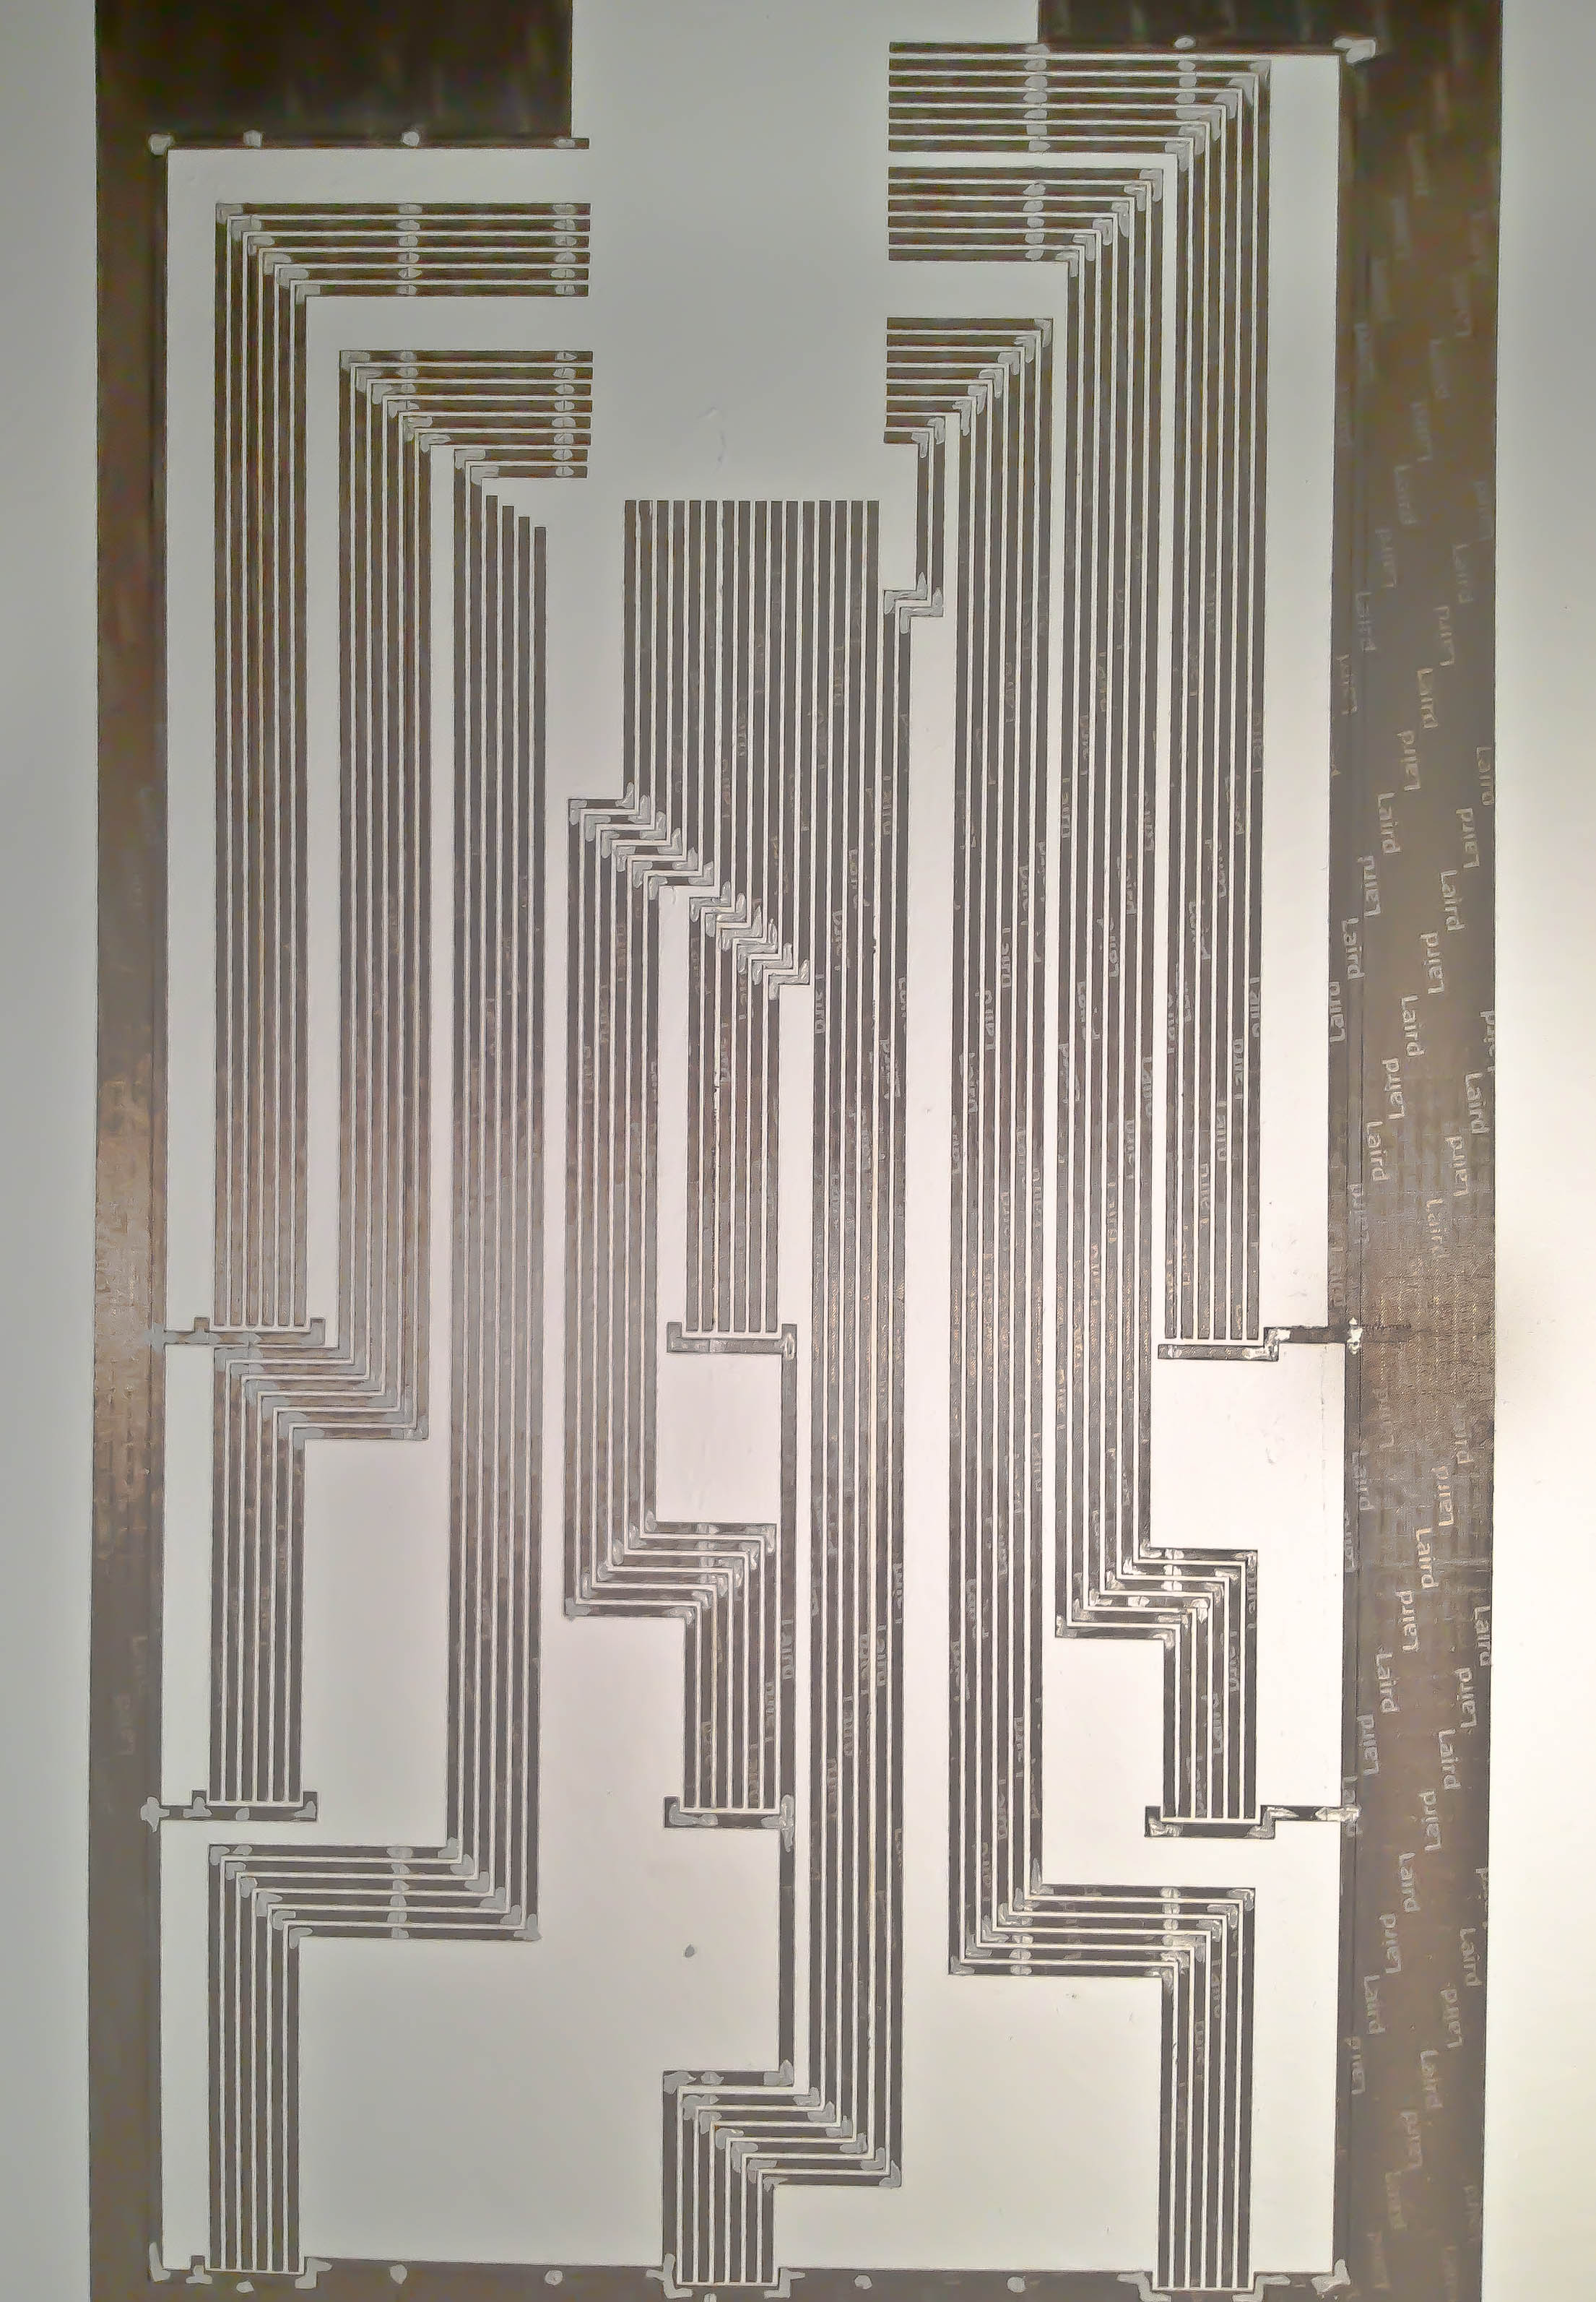
\includegraphics[height=.6\linewidth, angle=90,
width=3.6in]{images/popcad_circuit-3} \end{array}$
\end{center}
\caption{Two views of the conductive tape circuit connecting the paper towers
to the Arduino Mega microntroller. The circuit was constructed by laser cutting
a design through conductive tape (but not through the paper beneath it) and
removing the excess material.}
\label{fig:popcadCirc}
\end{figure}

In the first prototype, we still used traditional jumper wires from the Arduino
to connect to the headers beneath the towers, and 30 gauge (still traditional)
wire inside of the towers to connect from the headers to the LEDs and copper
tape. Admittedly, this does not feel very ``book-like'', or in the spirit of
faithfully exploring paper-based electronics. PopCAD v2 has no traditional
``wires'' at all. Instead, we use a fabric-based conductive tape, which, besides
laying flush (unlike wires) and feeling more like paper than copper tape, the
fabric tape is (unlike copper tape) able to be used in the laser cutter in our
lab. Figure \ref{fig:popcadCirc} shows two views of the PopCAD v2 circuit,
constructed by placing strips of the conductive tape on watercolor paper, laser
etching a circuit diagram through the tape (but not through the paper), and
peeling away the excess. This technique allows us to create a precise yet
completely flat circuit layout. The accuracy of this method permits the Arduino
Pro Mega (a thinner version of the regular Arduino Mega) to be affixed directly
onto the paper. The towers use this conductive fabric for the capacitive touch
sensors as well as material to solder the LEDs to, eliminating all the standard
wires from our design.

The software for the PopCAD retains all the algorithmic capabilities of the
SnapCAD version of the software (convex hull, path, minimal spanning tree), but
as the LEDs are affixed to the towers, we lose the ability for multiple player
functions. However, it should be noted that this was in part intentional; we did
not want any loose parts that could easily break, get lost, or other make the
device less portable. As it stands, the PopCAD (unlike its predecessors) is
self-contained as one piece, is small and light enough to be carried with one
hand, and is considerably less expensive (and less time-consuming) to produce.
We offered sample use cases for the previous devices that involved descriptions
of various technical features; for the PopCAD it seems more appropriate to
instead paint a more general user scenario that speaks to the intent behind
PopCAD's design. Imagine an art teacher, girl scout troop leader, hackerspace or
FabLab member, or any number of educators either wondering how to get into this
``3D printing thing'' or who have a Makerbot sitting in a corner gathering dust.
They find plans online (perhaps on Instructables\cite{Instructables} or some
similar DIY-oriented forum) for a relatively cheap, portable device that they
could not only turn into a group project to build with their kids, but once
built would offer a new way to introduce children to 3D modeling and 3D printing
in a completely new way. The democratization of digital fabrication technology
is (as stated earlier) a core goal of this work, and in many ways the PopCAD is
the device that embodies this ideal the most. So while it may be less expressive
or powerful in some ways (though as we point out in later chapters, this can
sometimes be an advantage), the PopCAD does have a place in our suite of
devices.




% \subsection{Discussion}
%  
% 
% Given the different medium of the pop-up book (paper as opposed to circuit
% boards), it is worth exploring the possibilities afforded by a cheaper, more
% flexible material. For instance, the flexibility of paper might provide the
% means for new types of modeling actions. It is plausible to imagine paper tabs
% or other mechanisms that perturb the LEDs off the integer lattice, or alter the
% overall topology in such a way that new shapes are possible (e.g. by deforming
% an equidistant grid into a spherical shape). There may be additional sensors or
% hardware that could be embedded into the book to provide new functionality
% (rotation, proximity, pressure). Additionally, due the inexpensive and portable
% nature of the pop-up book, it is worth exploring the sorts of interactions that
% could occur between several pop-up books (e.g., extending the input field to
% include two or more grids, networked interactions like cooperative modeling
% tasks, or competitive games like 3D-battleship). By using paper as a material to
% think with, we may find further possibilities as development continues.

\section{Software}
% \subsection{Software}
% 
% The UCube makes use of the Processing\cite{Processing} framework to read in
% the active coordinates from the Arduino microcontroller connected to the
% platform; the software then displays these as larger red points on a grid of
% grey dots. Users can rotate the grid along any axis by clicking and dragging
% with the mouse. In our current early prototype, there are only two buttons on
% the user interface: (i) an �export� button, responsible for taking the current
% set of active points and exporting them into "STL" file format (suitable for 3D
% printers), and (ii) a �mode� button which toggles between showing just the red
% dots as points and filling in an area (defined by a convex hull algorithm) to
% give a sense of shape.
% The software interface is intentionally minimal in order to encourage the user
% to focus on the physical interaction. We felt it was crucial not to fall into
% the trap of making another software tool for experts, so the main purpose of the
% software is to act as an aid�a means to cognitively clarify and confirm the
% user's intentions. Although it is likely that we will extend the software
% somewhat in future iterations, our goal is to support the physical experience of
% specifying a three-dimensional object, and not to add functionality beyond what
% is necessary or helpful to that end.

The software for the aforementioned devices utilizes the Processing Serial
library to read in the active coordinates from an Arduino microcontroller; it
then displays those coordinates on-screen as larger points against a ``ghosted''
grid of grey dots. The exact methods used to achieve this varied by device, and
were detailed in the device-specific sections above. This on-screen model can be
manipulated in a number of ways. Clicking and dragging along any axis rotates
the model, as does the use of the arrow keys on the keyboard.  Holding the shift
key while performing either action moves the entire model around the screen
(essentially re-centering it). The ``control'' key plus an up or down arrow key
zooms in or out along the z-axis. In addition to camera movements, there are a
limited number of functions represented by a simple graphical user interface
which aid and expand the modeling capabilities of the connected device.

For a brief overview of these functions, then: there are three ways of
interpreting the active set of points on the connected device: by taking the
convex hull of the input set, by connecting each point sequentially with a 3D
path, and by connecting the set according to a minimal spanning tree algorithm
(more on these modes soon). There is a single ``export'' button that will take
whatever the active shape is, no matter the mode (if there is one) and generate
a stereolithography file (.STL), the standard file format for 3D printing,
although .STL files can also be opened by more sophisticated 3D modeling
software, providing the possibility for the software to be used as a sort of
``sketchpad'' for rough ideas or shape that can refined afterwards. There is a
``close path'' button which will connect the first and last segments in an open
path (e.g. in constructing a square path, after the fourth point has been
placed, there will still be an open side of the square - pressing this button
will complete the square). There is an ``edit'' mode, whereby the real-time
input from the device is suspended in favor of being able to click-and-drag the
active points around with the mouse. Consequently, there is a reset button, in
the case that the user wishes to ``snap back'' to the normalized integer
lattice. There is also a slider element entitled ``path width'' that will
dynamically adjust each segment or branch width when in path or tree mode,
making the segments ``skinnier'' or ``fatter''. Finally, two minor aesthetic
options - the ``wireframe'' button will turn off the ``fill'' of the shape,
showing the outline stroke with a transparent fill, while the ``grid'' button
will toggle the visibility of the ghosted grid of non-active points.

% There are toggles for turning on and off the convex hull of the active points
% (either all the points or just the hull of a particular color), viewing the hull
% as a wireframe or solid object, and a toggle that shows or hides the background
% grid.  In addition, there are several import and export buttons: an export to
% STL (stereo lithography) format, the standard format for 3D printer files, as
% well as save and load options which allow users to save and re-load their shapes
% for use within the UCube system. Figure \ref{fig:software1} shows the UCube
% software upon reading in the eight points that were selected in Figure 1: in the
% bottom panel, the ``convex hull'' option has been chosen so that a solid cube is
% displayed (with the input points visible as the highlighted vertices of the
% cube). Now, by exporting this form (as mentioned above) to STL format, and
% sending the result to a 3D printer, we can produce a physical model of our
% specified shape, as shown in Figure 4.





% Before returning to the software itself, it is worth pointing out that, in
% effect, the events depicted in Figures 1, 3, and 4 constitute a typical scenario
% for employing the UCube. The user begins by selecting the vertices of a shape
% that she wishes to create (Figure 1); checks that shape against its appearance
% on the computer screen (Figure 3); and, if satisfied, sends that shape on to be
% output by a 3D printing device (Figure 4). There are, of course, limitations to
% this scenario - and we will touch upon these in the ensuing discussion.
% Nonetheless, it is the overall simplicity of the scenario that originally
% inspired the design of the UCube: the user need not construct a shape on a
% two-dimensional screen, nor be deeply familiar with the terminology and
% operations of modeling software. Instead, the creation of a desired shape takes
% place by moving one's hands in space.

As a guiding heuristic for our software design, it should be noted that the
device software is intentionally minimal. Our aim is not to produce another
sophisticated software modeling program - there are plenty of good ones
available already. Instead, the software is meant to aid the user in clarifying
their physical actions with the physical device, while maintaining a low barrier
to entry, a great possibility of expressiveness, and multiple ways of
approaching any given exercise - a trifecta of design heuristics often referred
to by Resnick (and others) as low floors, high ceilings, and wide
walls\cite{Resnick}.

\subsection{Modeling Modes} 

This section will describe the three main modeling modes of the software, with
particular attention to explaining the methods by which they form shapes, the
algorithms behind how they operate, and the modeling domains for which they are
particularly suited.

\subsubsection{Convex Hull: Creating Polyhedral Forms} 

In observing a set of lights placed on an integer lattice in 3-space, one of the
first mental images we thought of was to take the convex hull of that set and
create a solid polyhedral form. One may think of the 2-dimensional convex hull
as the operation performed on the 2D geoboard mentioned earlier in the chapter;
given a randomly scattered set of nails in a board, the convex hull of those
nails will be equivalent to a rubber band that stretched around all the points.
That is, the minimal form that includes all of the line segments connecting each
pair of points, as the rubber band forms a straight line between those nails on
the hull as opposed to curving inward (thus the minimal shape of line segments
as opposed to area). In three dimensions, this becomes a convex polyhedron
instead. Many popular 2-dimensional convex hull algorithms originated in the
early 1970's (e.g. Jarvis March/Gift Wrapping, Graham Scan), while a
3-dimensional solution was published in 1977\cite{preparata1977convex} and
popularized by the same author in the book, \emph{Computational Geometry: An
Introduction}\cite{preparatat1985computational}.

The version implemented in our program is a derivative of the work presented in
\cite{barber1996quickhull}, and adapted from the implementation at \cite{quickhull3d}
which combines a 2D Quickhull Algorithm with a general dimension Beneath-Beyond
Algorithm to achieve a general dimension convex hull solution. In brief, the
strategy works as follows: (a) from a given set of input points, where the
coordinates are known, create an initial 3-simplex (tetrahedron) - from the
min/max points in along each dimension (x,y, and z), and add the four faces of
the tetrahedron to the stack, (b) Pop a face from the stack and get the point
most distant to that face, (c) Find all faces adjacent to the selected face,
find the horizon edges of the adjunct faces and extrude the shape along those
edges to the selected point. (d) Put the newly discovered faces on the stack and
repeat from (b) until all points have been accounted for.

When the hull mode is active in the software, the coordinates on the connected
device must be sent to the hull construction methods each time a point is added
or removed to ensure that the hull remains accurate in real-time. The worst case
for this algorithm is $\Omega(n^2)$, although in practice is not worse than
$\Omega(n$ $log$ $n)$. Figure \ref{fig:software1} shows two screenshots of a
``before and after'' convex hull computation in the software in which the
picture on the left in simply displaying the active set of points, while the
figure on the right shows the interpretation of those points after clicking the
convex hull button.


\begin{figure}[ht] \begin{center}$
\begin{array}{cc}
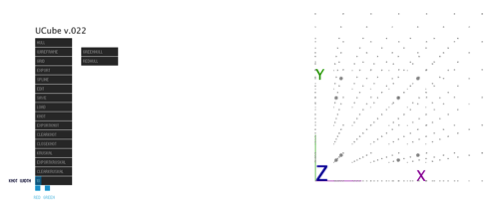
\includegraphics[width=.47\linewidth]{images/software_1} &
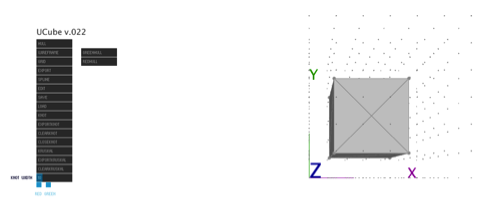
\includegraphics[width=.47\linewidth]{images/software_2}
\end{array}$
\end{center}
\caption{Two screen views (left and right) of the device software, illustrating
the way in which the software displays the convex hull of a cube. Left: The set
of eight input points, before the ``Hull'' button has been pressed. Right: The
resulting convex hull, forming a cube from the input points.}
\label{fig:software1}
\end{figure}

Polyhedral forms obviously have a long history not only in modeling, but in
geometry (the Platonic solids), architecture (the Pyramids of Egypt), and
numerous other disciplines over the ages (building blocks, paper crafts, etc.).
Though not all the Platonic solids can be modeled naturally (i.e. without edit
mode) on our devices, certainly pyramids can be, as well as other common convex
polyhedral shapes (e.g. a canonical ``house'' consisting of a cube with a
tetrahedron sharing the cube's top face). Some examples are shown in Figure
\ref{fig:hulls} below.

\begin{figure}[ht]
\begin{center}
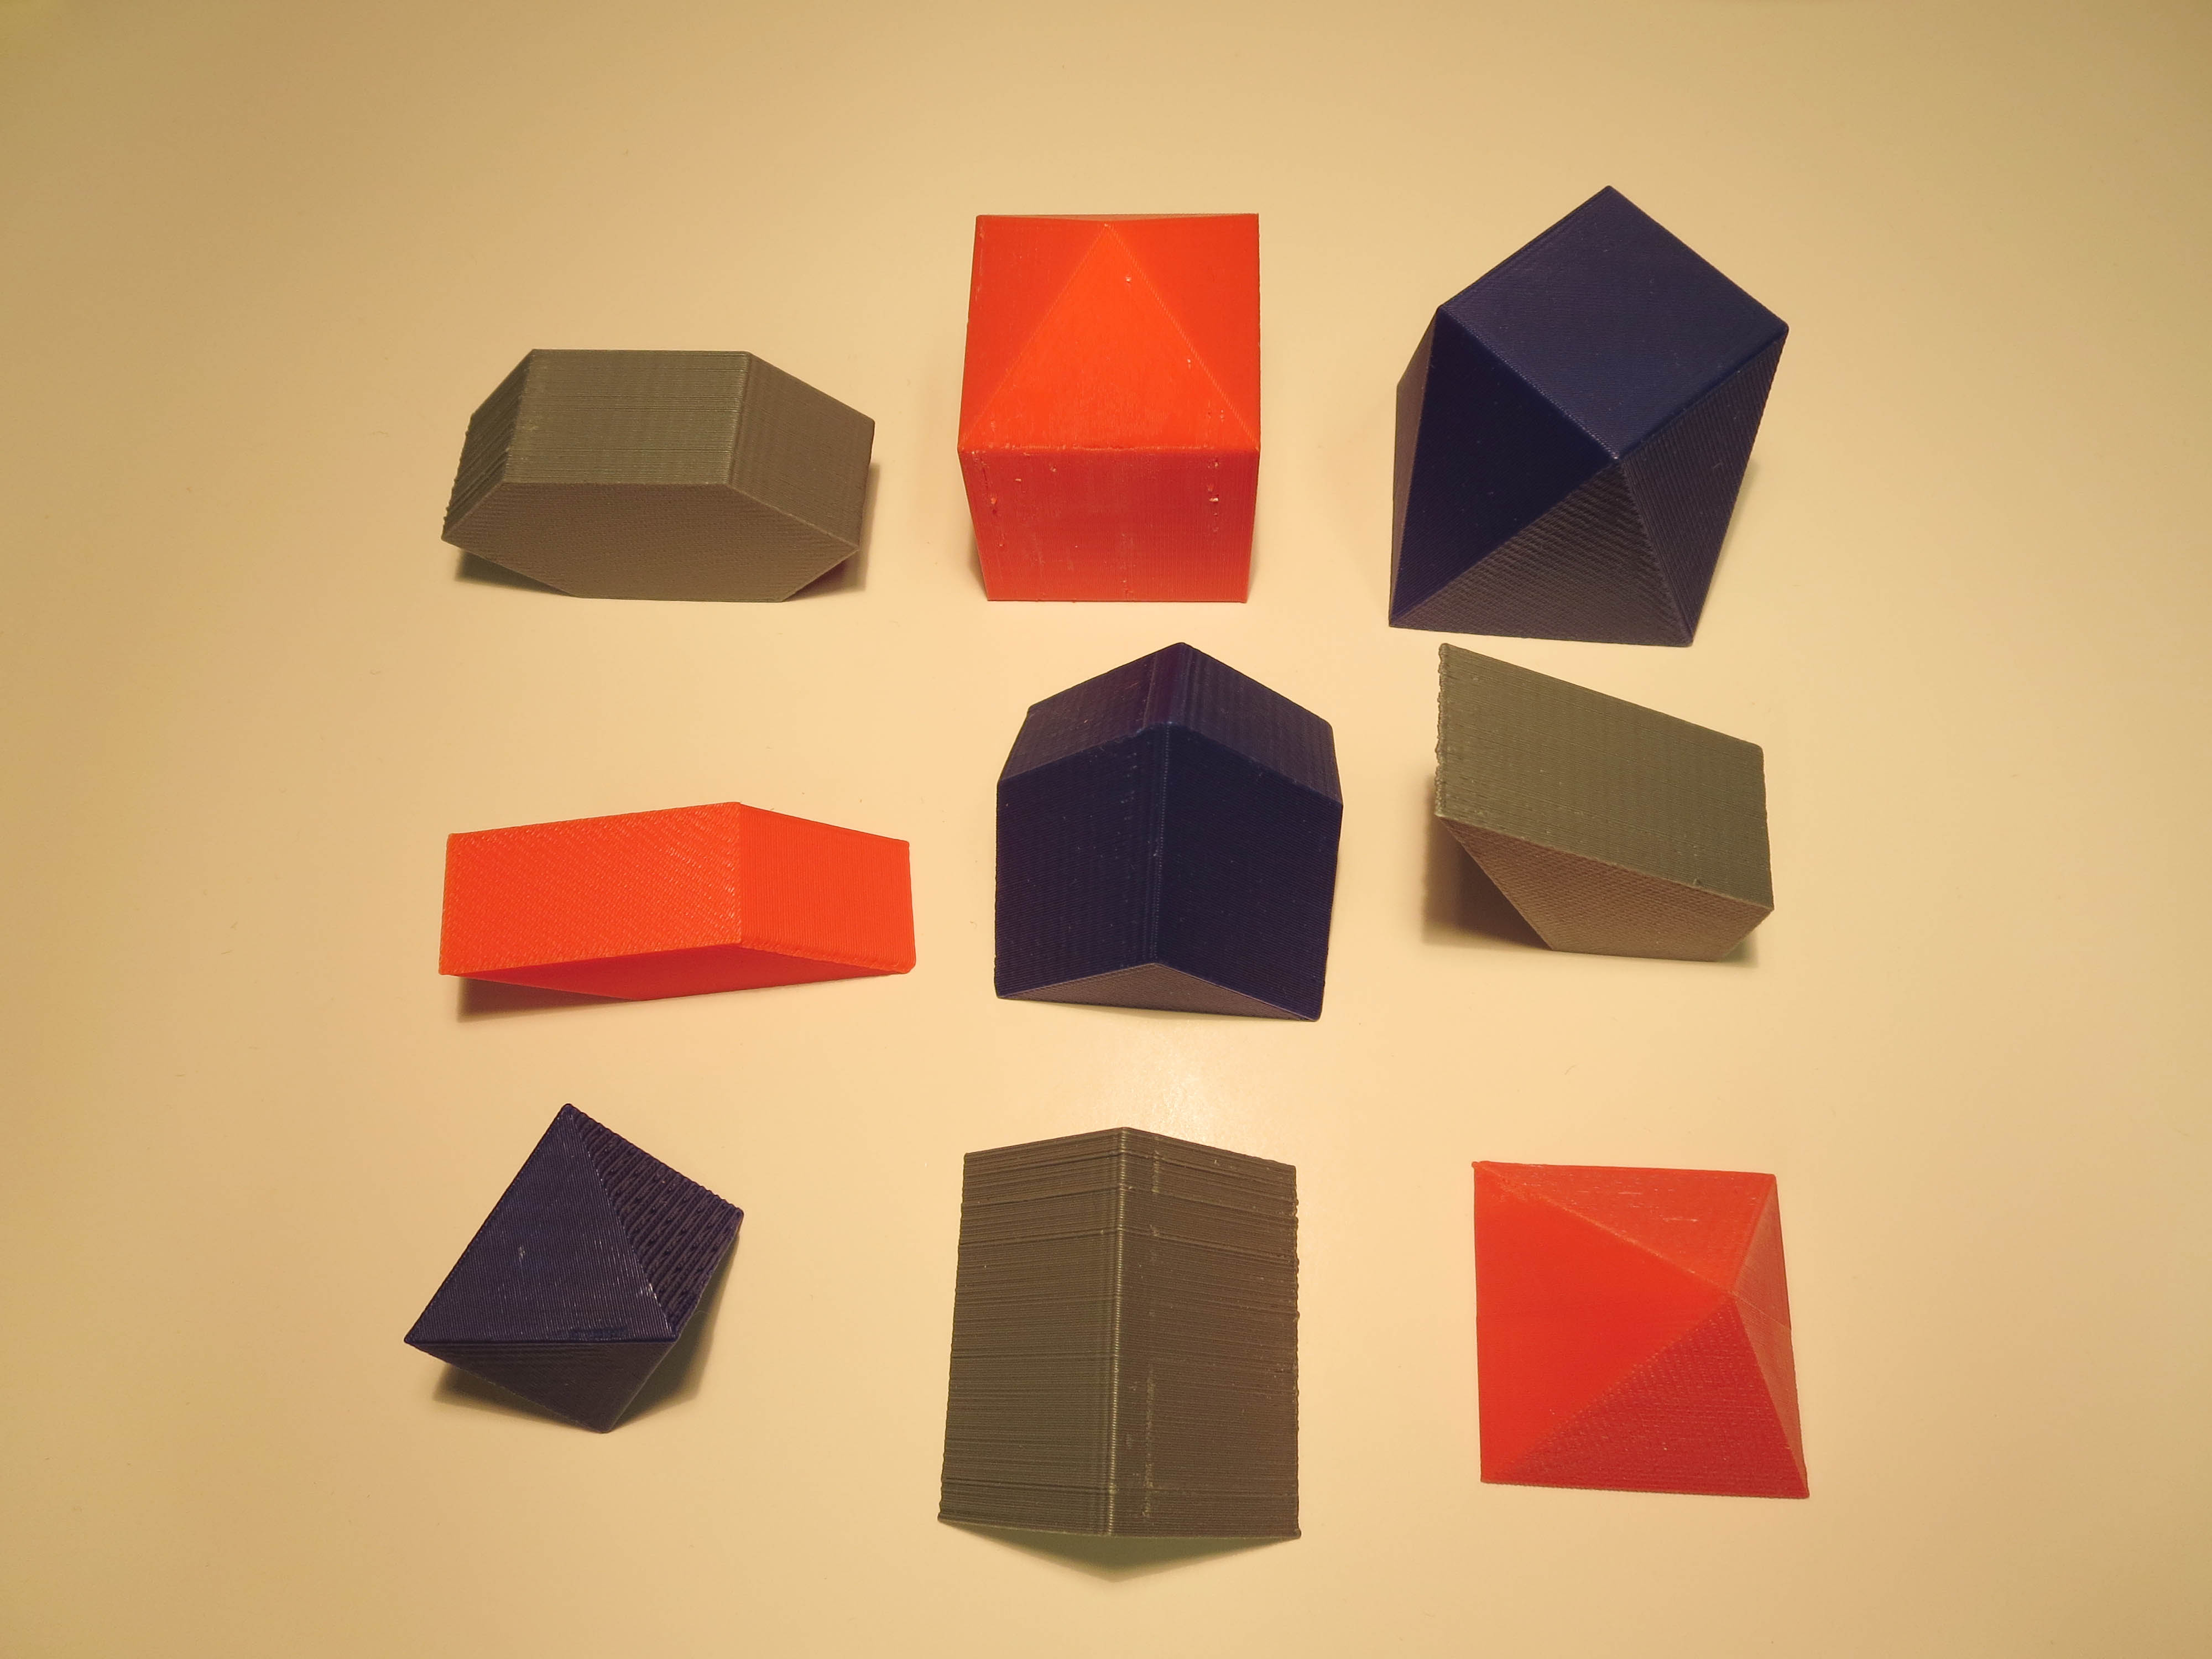
\includegraphics[width=.5\linewidth]{images/hulls}
\end{center}
\caption{A collection of 3D printed shapes modeled using the convex hull mode in
the software with the devices mentioned earlier in this chapter.}
\label{fig:hulls}
\end{figure}



\subsubsection{Paths: Creating Linear Forms and Knots} 
In the convex hull examples in the previous paragraphs, we have not made use of
the fact that the software samples selected points in real time: thus, when a
user adds or subtracts a point in space, that change is registered immediately
in the desktop software. What this means is that the user can exploit not only
the overall set of selected points, but can also make use of the \emph{order} in
which those points are selected. A sequence of selected points need not
represent only vertices of a solid; it can also represent a path over time in 3D
space. Figure \ref{fig:paths} shows several sample projects based on this idea.
Here, the software has been employed to read points as successive positions of
various routes through 3-space. The resulting paths have been printed out on a
3D printer.

In some cases, the path is closed, finishing at the same location where it
started; the path printed out at center in red in Figure \ref{fig:paths} is in
fact a well-known mathematical form, a trefoil knot. (It may be worth mentioning
here that such a knotted form would be rather tricky to create in standard 3D
modeling software, but the form can be created ``by hand'' with our devices,
selecting light positions in space along the path of the knot.)

\begin{figure}[!ht]
\begin{center}
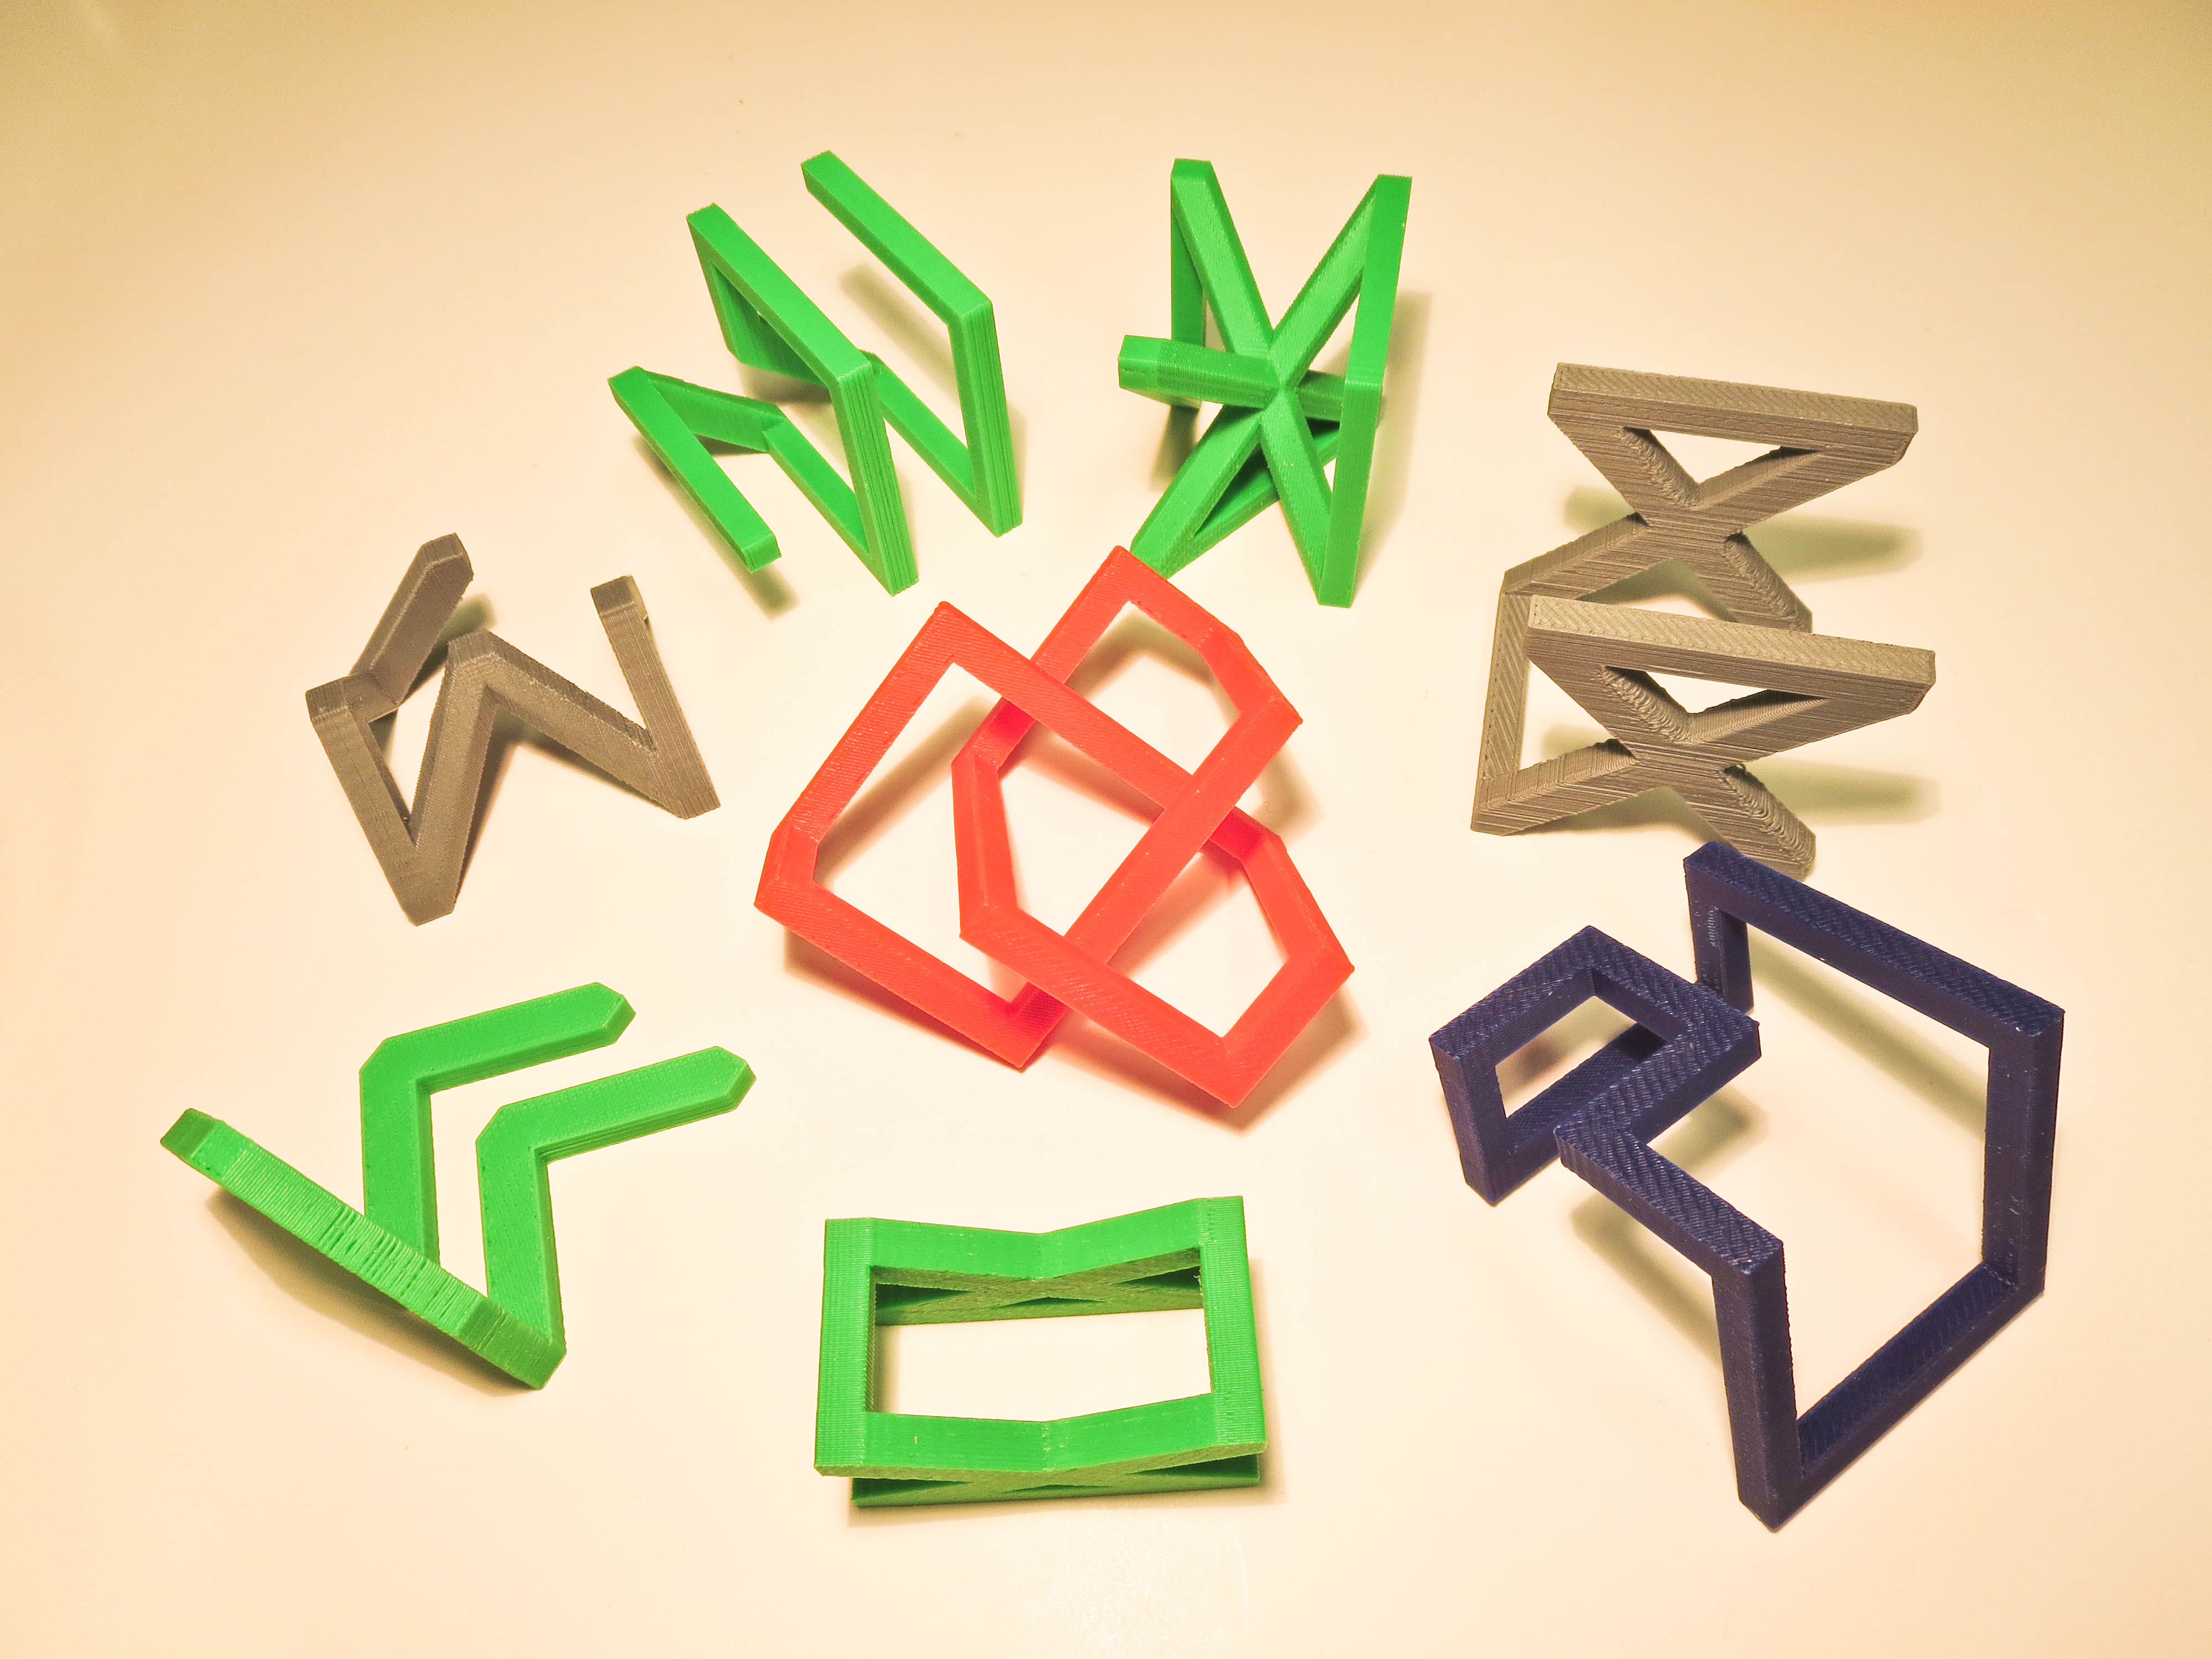
\includegraphics[width=.5\linewidth]{images/paths}
\end{center}
\caption{A collection of paths modeled on our devices using the path mode in
the software, exported from the software and 3D printed in our lab. The red
shape in the middle may be recognizable as a traditional trefoil knot.}
\label{fig:paths}
\end{figure} 

To briefly explain the workings of this mode, then: each point on the device is
stored, in order, in an array. Once the second point of the path is added (one
point a path does not make), each point is then ``exploded'' into a cube,
centered on the point. The size of each cube is controlled by the ``path width''
slider, so the single original point generates 8 points, offset by the current
value of the path width slider (e.g., Point p1 = new Point(x + offset, y +
offset, z + offset);). The algorithm then takes the cube of points associated
with each pair of connected points (e.g., points 0 and 1, 1 and 2, 2 and 3,
etc.) and runs the convex hull algorithm discussed earlier, generating a sort of
rectangular prism between the two cubes. By connecting each new point to the
previous one, a trail of rectangular prisms is generated between the points
specified, in the order in which the user placed them. Figure
\ref{fig:trefoilPath} shows a trefoil knot created with the path mode. By
highlighting the strokes in red, one can see that each point is in fact
surrounded by a cube, while each cube is connected to its neighbors by
rectangular prisms.

\begin{figure}[!ht]
\begin{center}
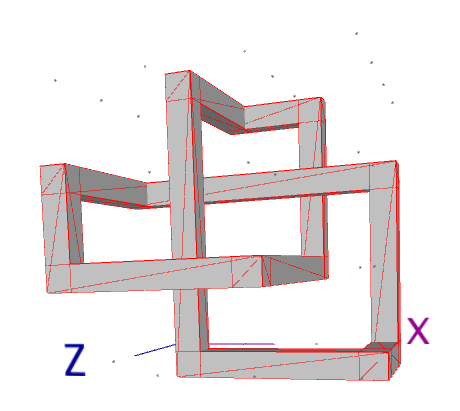
\includegraphics[width=.5\linewidth]{images/trefoilPath}
\end{center}
\caption{A trefoil knot, as modeled on the UCube version of the software.
The outlines (strokes) of the knot have been highlighted in red to show the
manner in which the software constructs the path; points are expanded into
cubes, and adjacent pairs of cubes and then connected with rectangular prisms
(the convex hull of two separated cubes).}
\label{fig:trefoilPath}
\end{figure}

The utility in creating a mode like path is fairly self-explanatory; it allows
for a vast number of shapes to be modeled, of a wholly different class of
objects as the traditional polyhedral style of the convex hull output. As we
will discuss in greater detail later, this method was popular with children who
used it; in some ways it is akin to writing or drawing, albeit in 3D, where once
you have a pen on paper, a line will follow wherever you move your hand. The
path mode allows for the creation (or close approximation) of most English
letters and numbers, common symbols (like stars), and 3D outlines of normally 2D
geometric shapes, like triangles and rectangles.


\subsubsection{Points as ``Blocks'': Creating Non-Convex Polyhedral Forms} 
Aside from the convex hull and path operations noted above, the device allows
for multiple different semantics for spatial locations. For example, in the path
mode previously mentioned, if we choose to construct paths with an edge-length
of one ``interval unit'' of the given device - achieved by putting the software
in path mode and setting the ``path width'' slider to one-half of the distance
between points - each cube created will fit perfectly next to its neighbors,
turning each point into a sort of ``block'' . In this way, selecting (say) four
successive light locations along the length of one tower, then, one could
specify a rectangular prism. Likewise, by selecting three point locations in an
``L'' form, one could specify the non-convex polyhedral form seen at the far
left of Figure \ref{fig:soma} below.
 
\begin{figure}[ht] \begin{center}$
\begin{array}{cc}
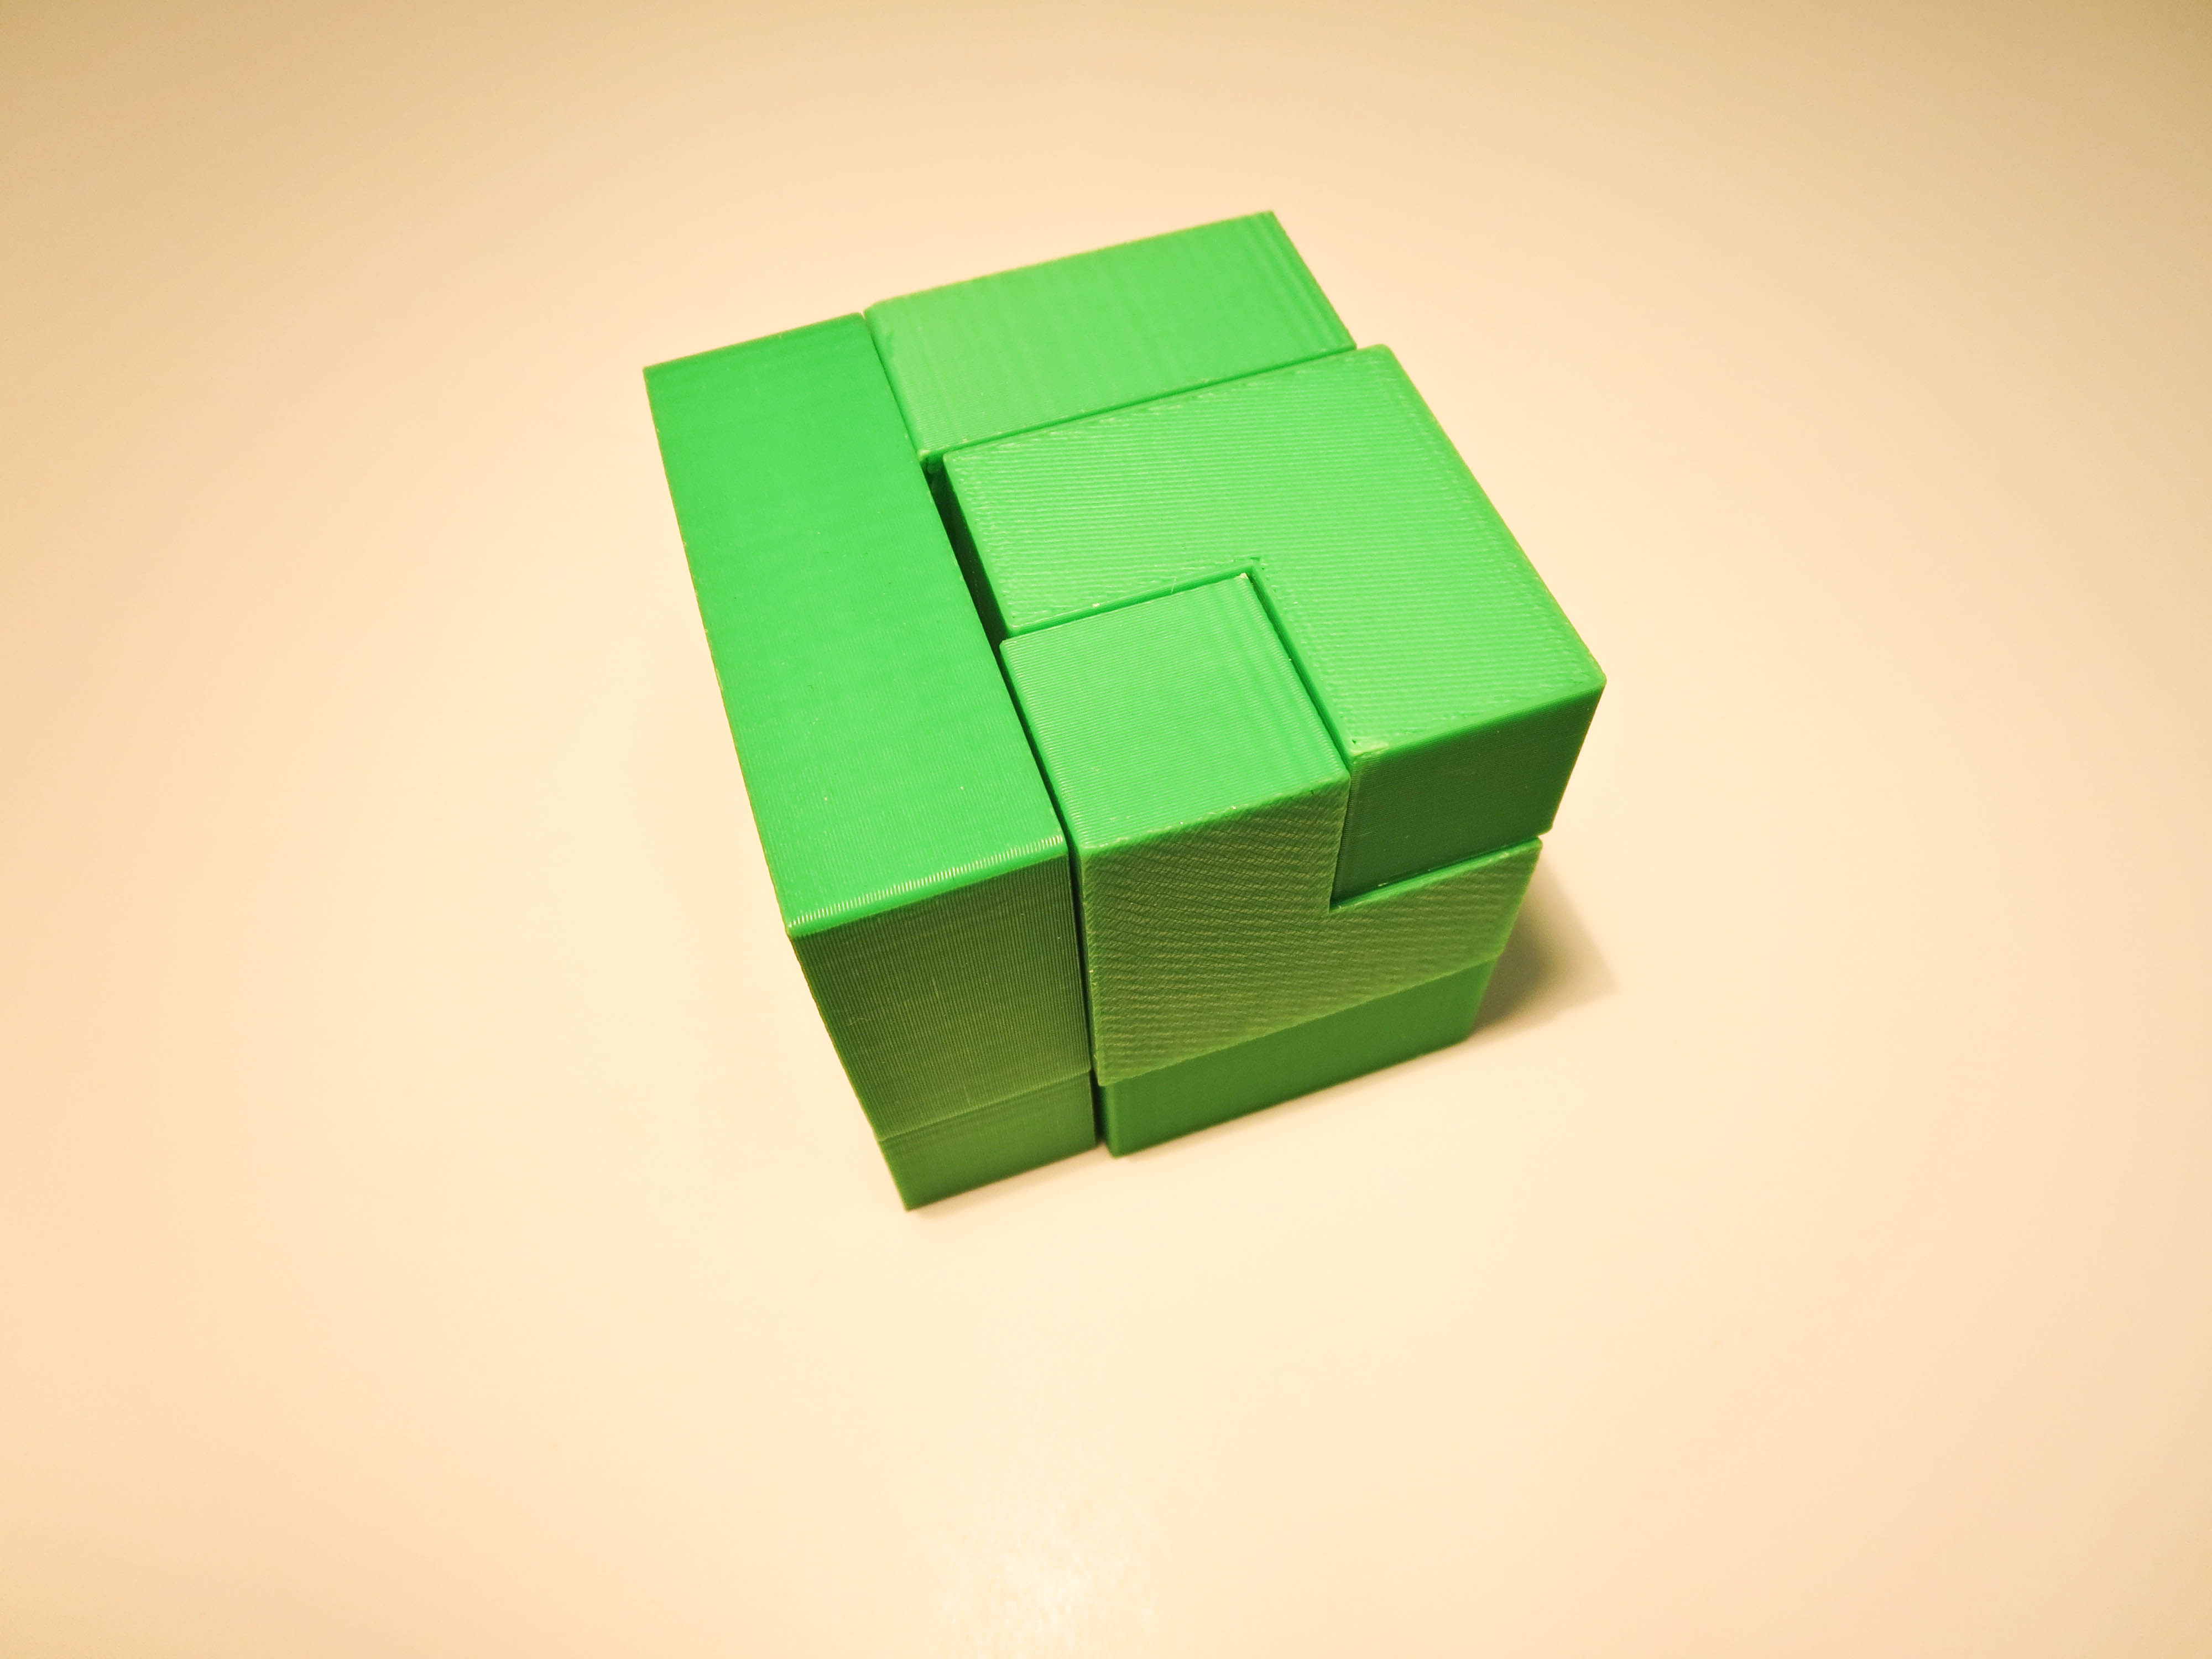
\includegraphics[width=.46\linewidth]{images/somaCube} &
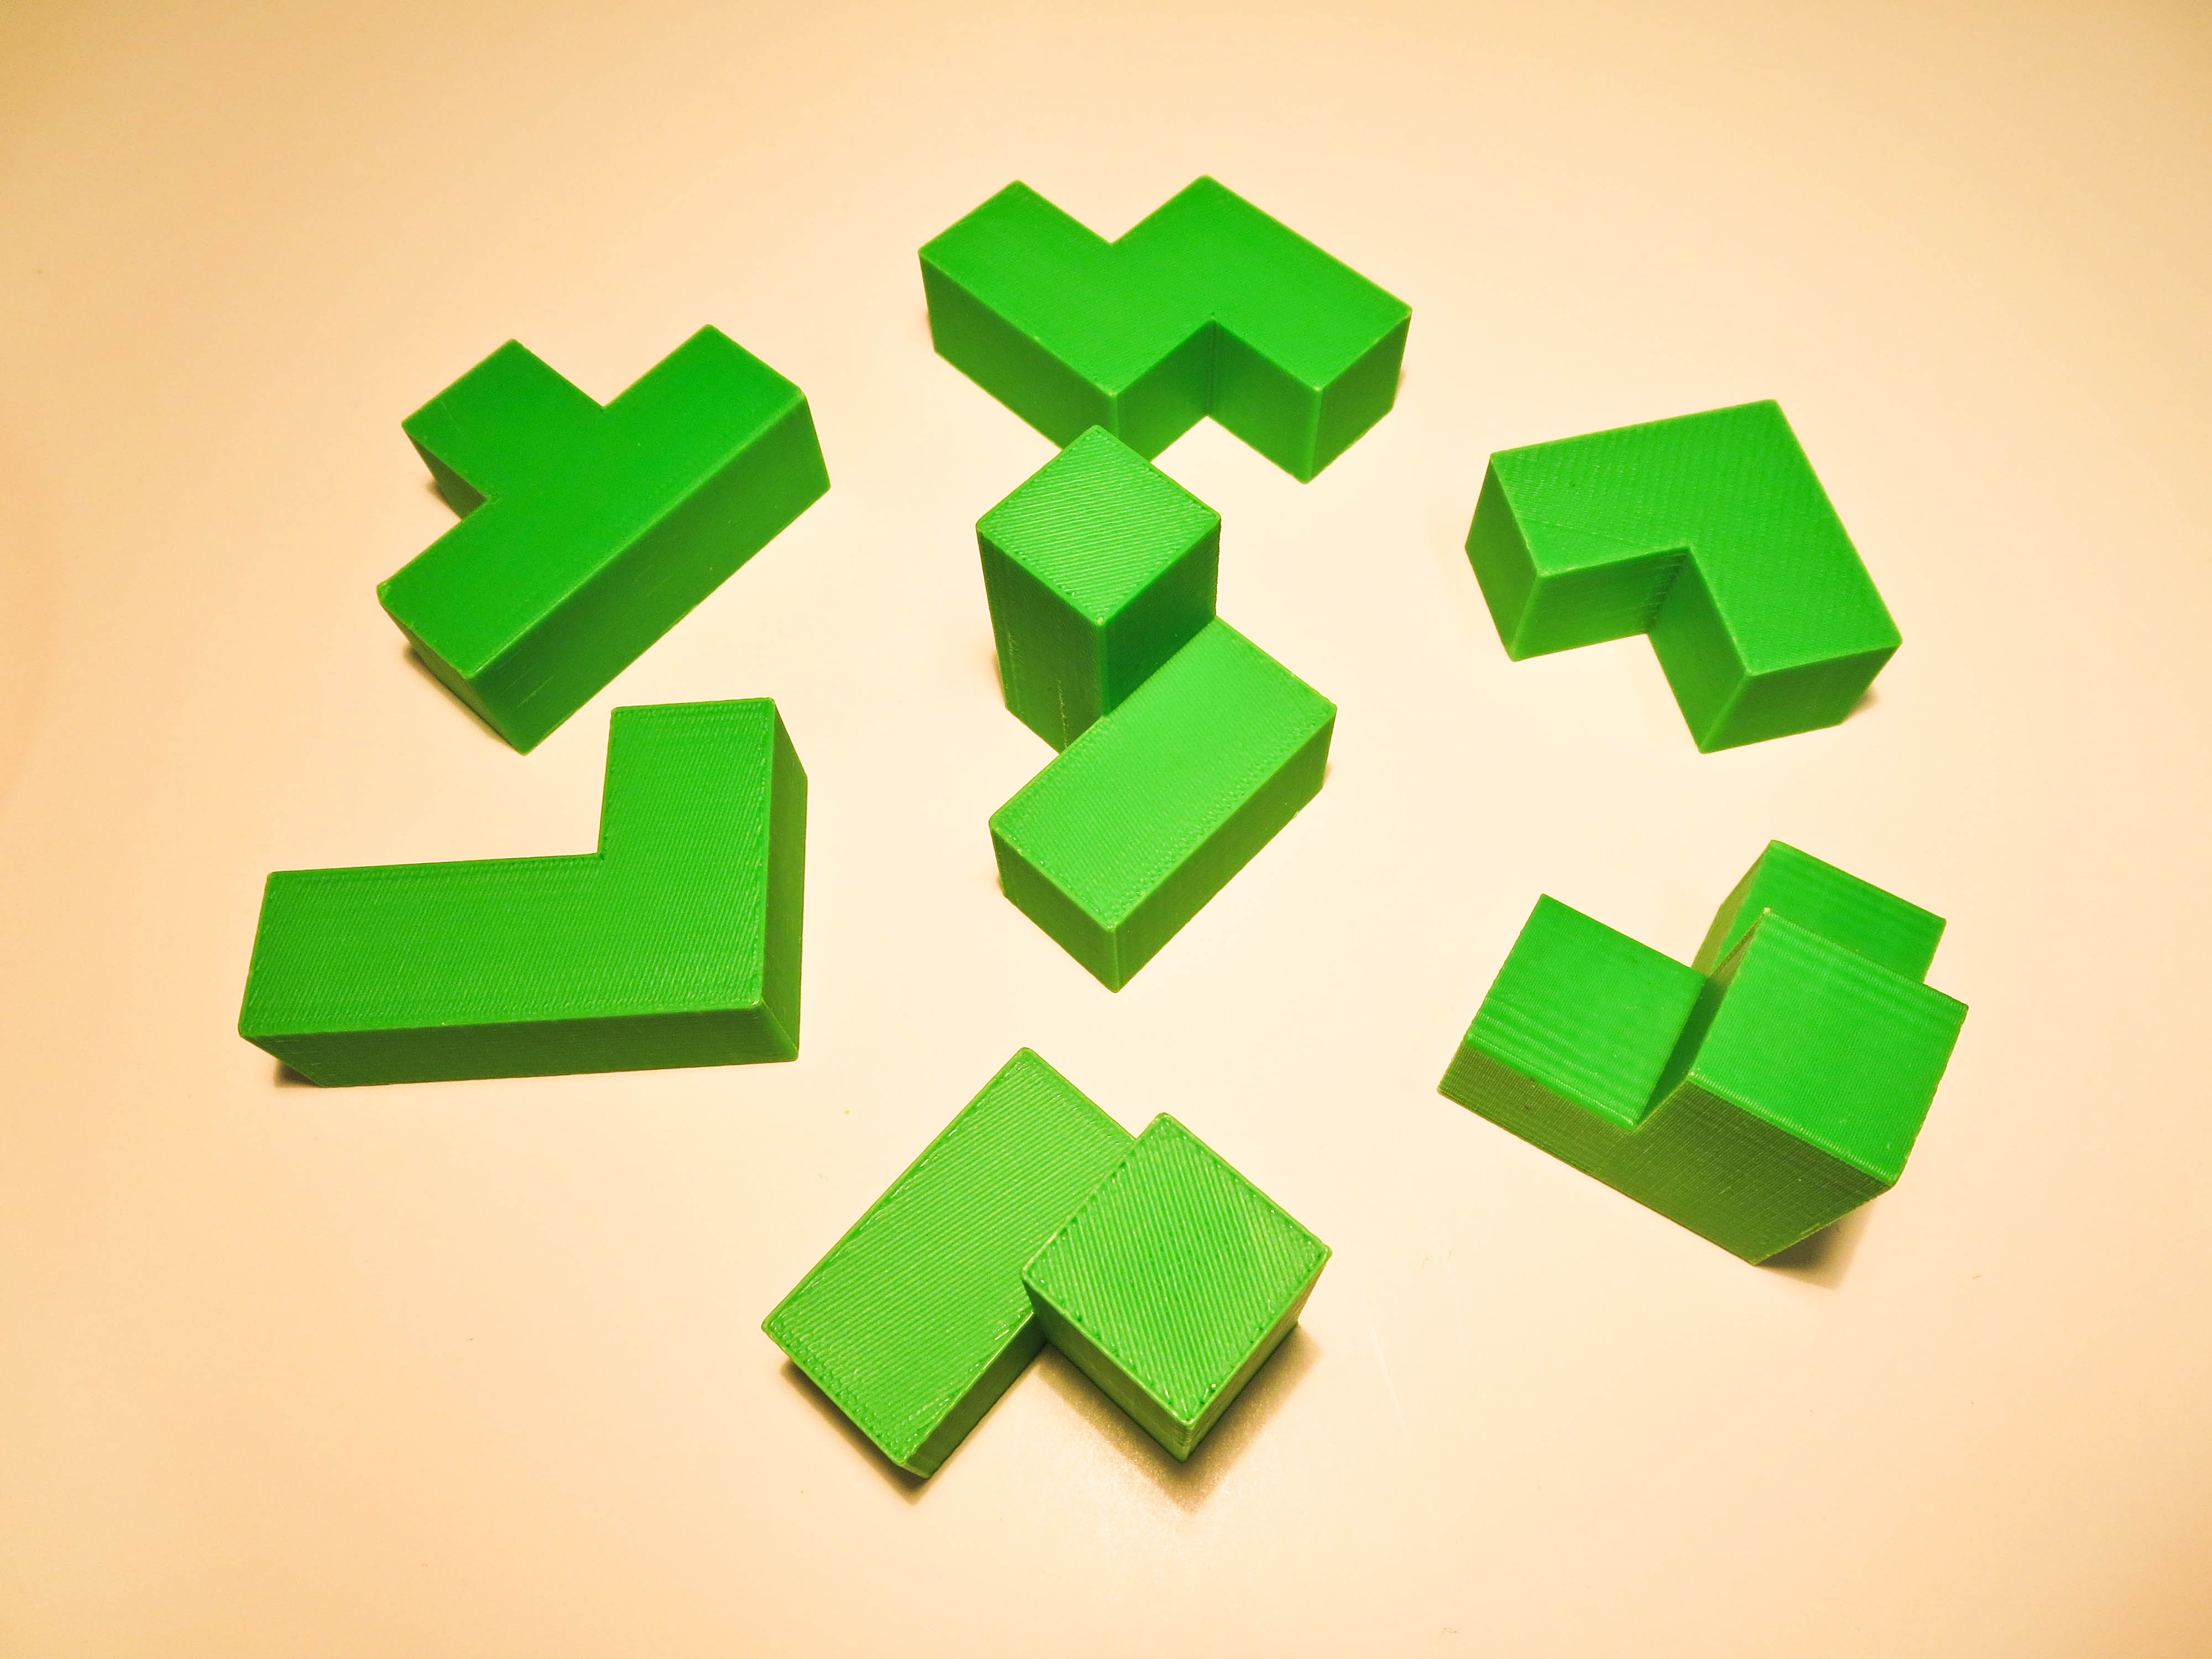
\includegraphics[width=.46\linewidth]{images/somaPieces}
\end{array}$
\end{center}
\caption{A set of non-convex polyhedral forms modeled on the UCube, which
constitute the well-known ``Soma Cube'' puzzle, shown assembled on the left
with the individual shapes laid out on the right.}
\label{fig:soma}
\end{figure}

This technique for using the path mode has some interesting advantages in terms
of the physical properties of the paths produced in this manner. For those
readers interested in recreational mathematics, the shapes shown in Figure
\ref{fig:soma} will be recognizable as the component pieces of the ``Soma''
puzzle; these pieces can be arranged together to form a larger cube (also shown
in \ref{fig:soma}). The software could be employed with any of the devices in
similar fashion to produce many such dissection-type puzzles, building blocks,
or other for other domains where interlocking, block-like shapes may be useful:
architectural mockups, model train environments, real-life Tetris, and a myriad
more.

\subsubsection{Point Clouds: Creating Minimal Spanning Trees}
Instead of interpreting points as vertices of a solid (as in the convex hull
examples) or as the successive stations of a temporal path (as in the ``path''
examples above), we could in fact simply treat our set of points as just what
they are � namely, a set of points. Starting with this interpretation, we might
produce a form such as a minimal spanning tree of the set of points (a set of
edges of minimal total length connecting all the points). Figure \ref{fig:trees}
shows several examples of forms created this way; one immediately grasps the
variance and complexity that this mode is capable of. The yellow ``jack'' in the
middle of \ref{fig:trees} is the product of nine points, eight of which form the
equidistant vertices of a cube (or what would form a cube if the software were
in convex hull mode), with the last point perfectly centered in the middle,
effectively ``bending'' the rest of the graph segments in to meet it.

\begin{figure}[!ht]
\begin{center}
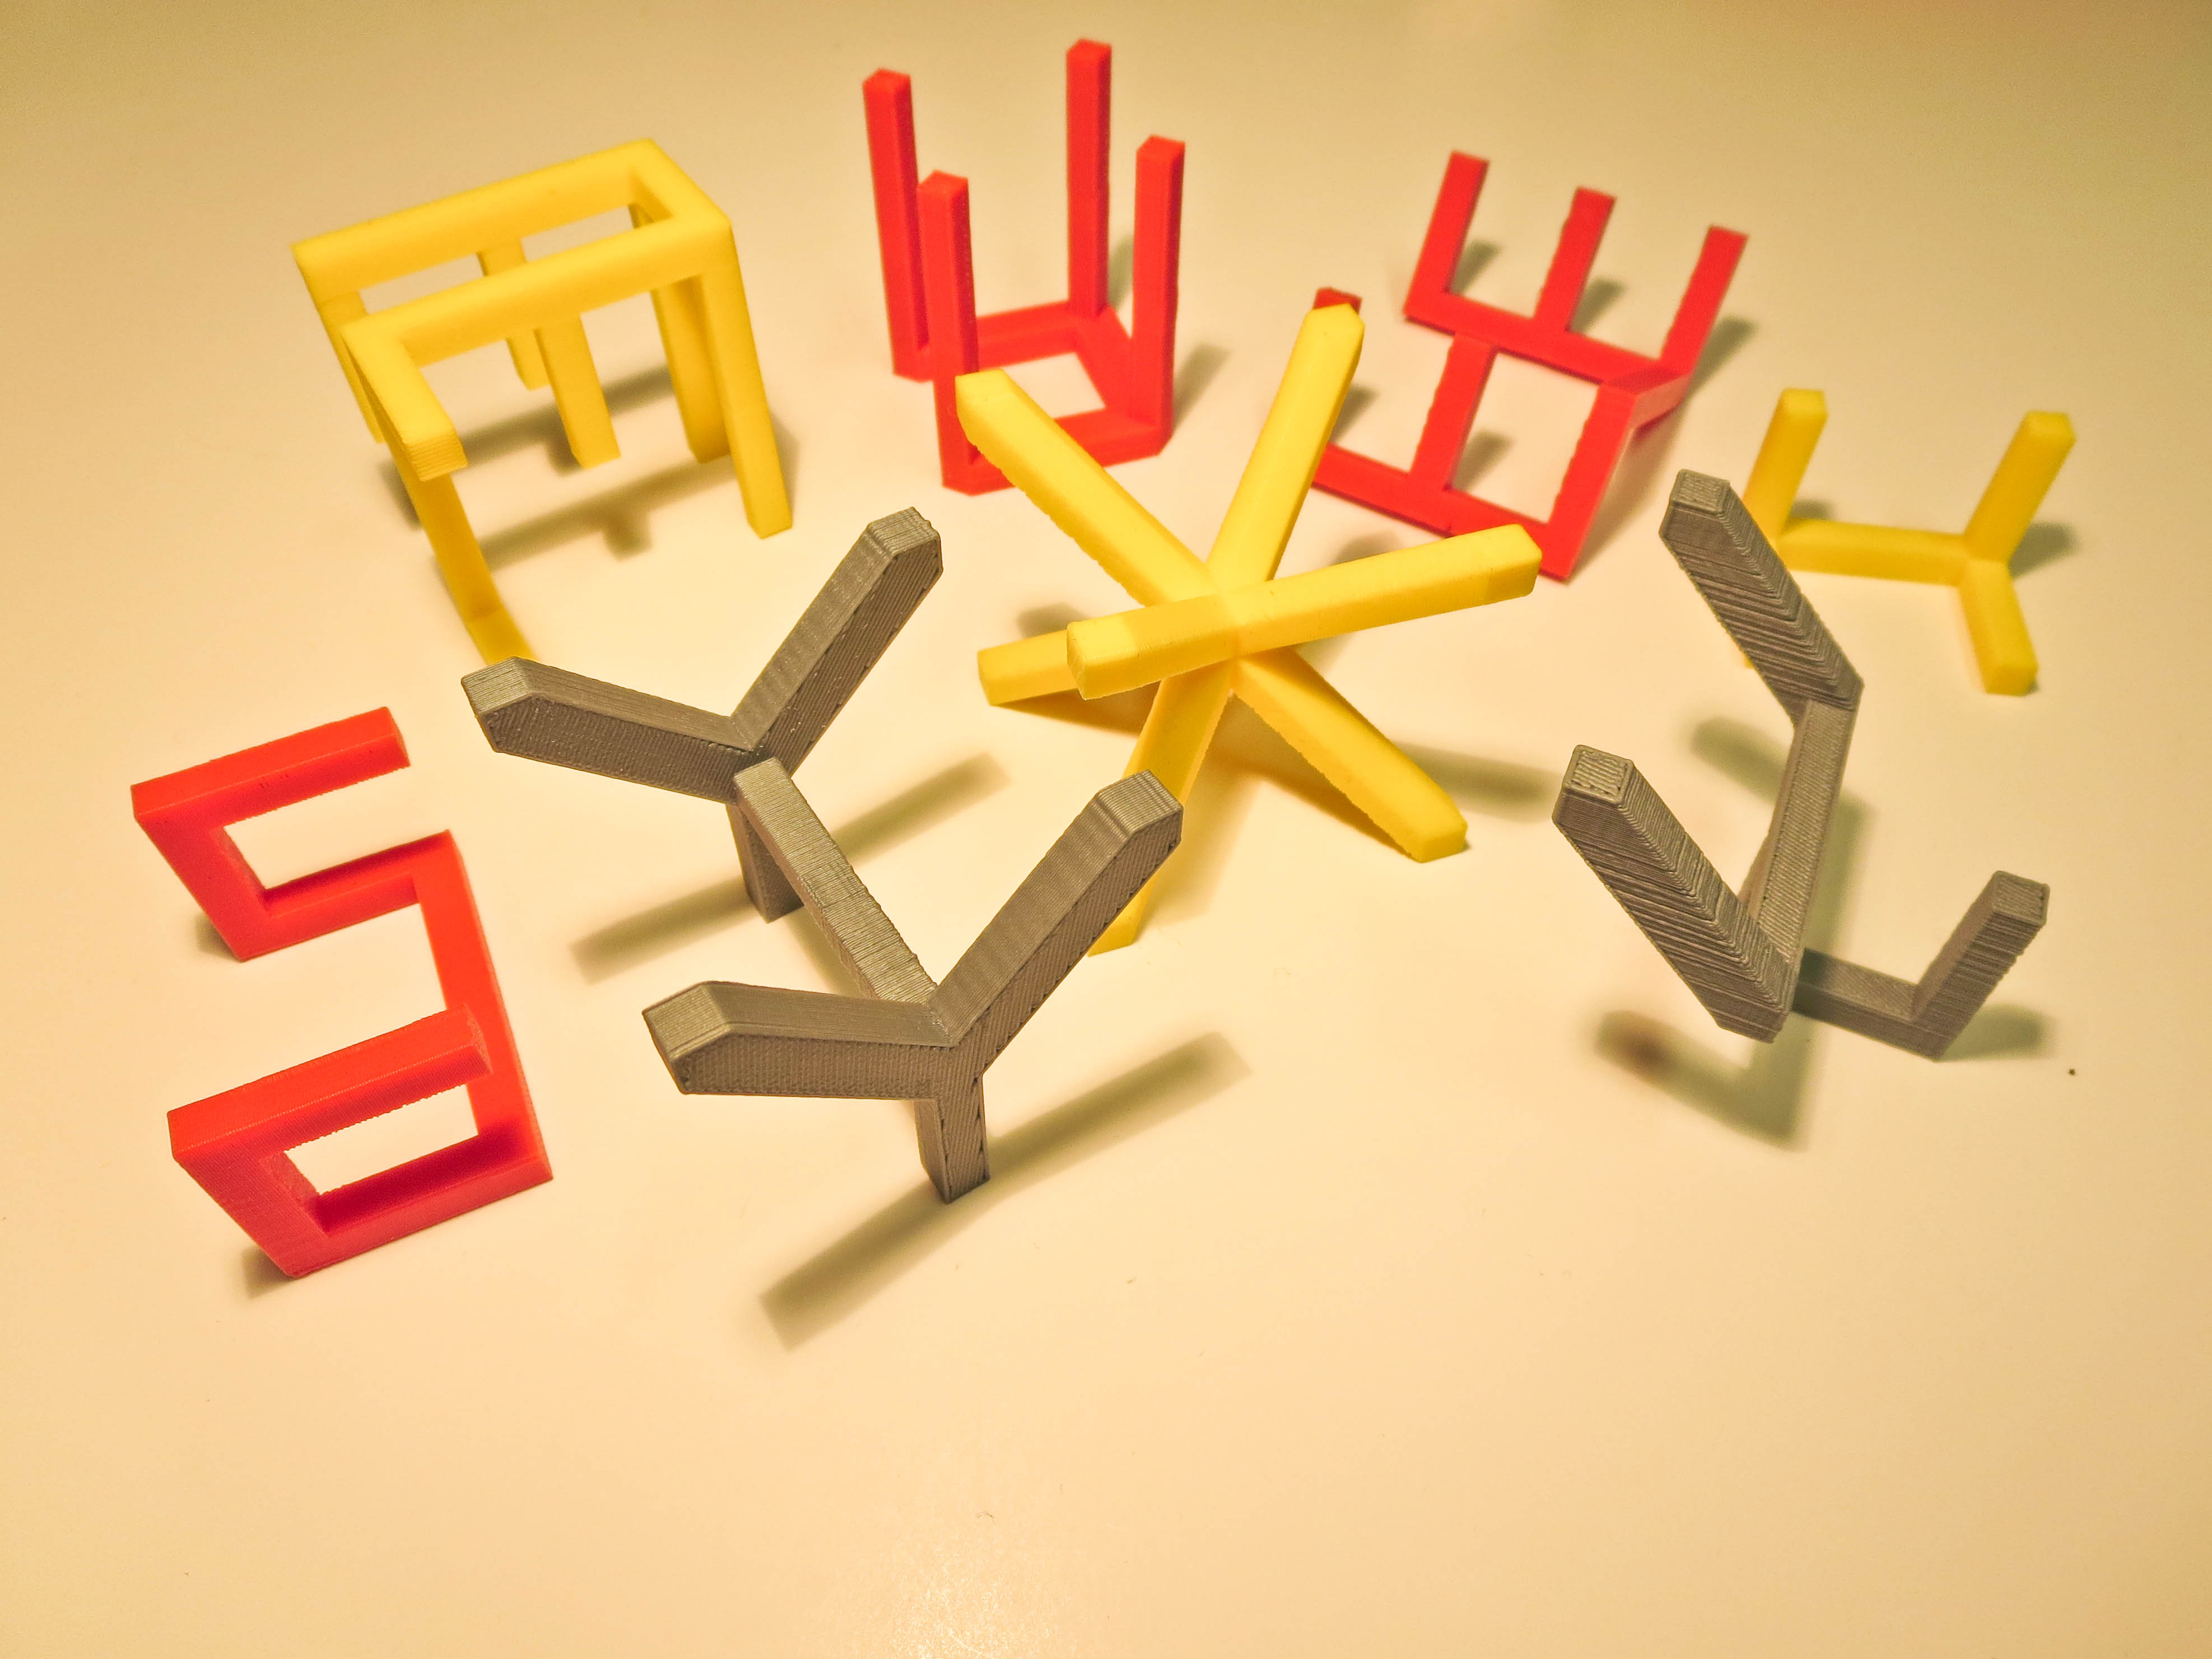
\includegraphics[width=.5\linewidth]{images/trees}
\end{center}
\caption{Several examples of models produced using the minimal spanning tree
mode in our software, exported, and printed out on a 3D printer.}
\label{fig:trees}
\end{figure}

As with the convex hull, the minimum spanning tree is a well-defined,
extensively studied algorithm in computer science and mathematics. Given a set
of points on a graph, the minimal spanning tree will be a solution (possibly
more than one) that connects each point on the graph, without cycles (returning
to a point already in the tree), and with the minimal possible value of some
``cost'' variable, often defined as the sum of ``weights'' of the connected
edges in the tree. One may think of the minimal spanning tree like constructing
a subway system, where all the stations need to connect and the length of
track should be minimized to keep construction costs as low as possible.

The first algorithm for finding the minimum spanning tree was derived by a Czech
scientist, Otakar Bor\r{u}vka in the late 1920's\cite{boruuvka1926jistem}, for
the purpose of planning electric distribution networks. There are two popular
algorithms used today, Prim's and Kruskal's both of which are considered
``greedy'' (by iteratively choosing the locally optimal edge to determine the
spanning tree) and run in polynomial time.
Our software uses an implementation of Kruskal's algorithm, whereby Euclidean
distance between two points on the graph is used as that connecting edge's
weight. Kruskal's algorithm, first described in 1956\cite{kruskal1956shortest},
starts by taking a set of each vertex (thought of as separate trees) and a set
of all the possible edges in the graph (with their corresponding weights), then
iteratively removes the edge with the lowest weight from the set of edges and
adds it to the set of vertices, connecting two of these trees into one, until
there is only one tree left from the original set of vertices (or we run out of
edges to pull from). If there is only one tree left in the vertex set, then that
tree represents the minimal spanning tree. It is, of course, possible to have
more than one minimal spanning tree for a given graph however.

In our software, we run Kruskal's algorithm whenever a point is added or removed
in ``tree'' mode. The set of points is sent as inputs, the edges and edge
distances are calculated, the algorithm is run, and returns a list of connected
edges, the set of which is the minimal spanning tree. This list of edges is
treated in much the same way as the points in ``path'' mode: each edge has two
point coordinates, both of which are ``exploded'' into cubes centered on the
point, and then the set of two cubes (16 points) are sent to the convex hull
algorithm, creating a 3D rectangular prism between the two cubes.

Including the minimal spanning tree mode is an interesting departure from the
convex hull and path modes; it is not easily explained to the novice designer,
nor does it have the sort of intuitive relationship to the set of active lights
as the other modes do. The addition or subtraction of a single point can
radically alter the resultant spanning tree in (sometimes) unexpected ways - not
so with the convex hull or path modes. However, it is this lack of immediate
understanding and the element of unexpectedness that makes this mode a good fit
for the kind of devices we make. The real-time adjustments of the software in
combination with the exploratory nature of the devices makes the tree mode
highly engaging (in our observations, explained in full later on). The ability
to quickly add or remove points from the graph is a feature unique to our
devices and allows for a quick way to ``check and see'' different combinations
of points and strategies, while being able to look between the device and the
software and start to draw some conclusions about how their actions affect the
shapes being displayed.

\subsection{Other Software Functionality}

The software modeling modes mentioned in the last section set the stage for the
types of figures that can be constructed with our devices, the software has
additional features that are crucial to the overall purpose of the system. This
section will go over the operation and methodology of the most important of
those: the software's ``Edit'' mode and the ``Export'' feature, allowing figures
to be saved in a 3D-printer friendly format.

\subsubsection{Edit Mode}

In order to (partially) address the ``inflexibility'' inherent in having points
and thus shapes confined to the integer lattice, we developed a way in the
software to ``edit'' the points by putting the software into a special mode that
freezes the serial input from the connected device and allows the user to
click-and-drag points off their ``hardware defined'' locations. The edit mode
affects all three of the modeling modes mentioned above, so the user can how the
edits they make change each modeling algorithm. We also provide a ``reset''
button as a way to ``snap'' back to the original grid of points.

The mode works by combining several pieces of functionality that work together
to keep track of the cursor position (to detect if it is hovering over a point)
and its click-state, track the relative position of the point as it is being
moved, and relay that position information to the data structures responsible
for the different modeling modes - all in real time.

\begin{figure}[!ht] \begin{center}$
\begin{array}{cc}
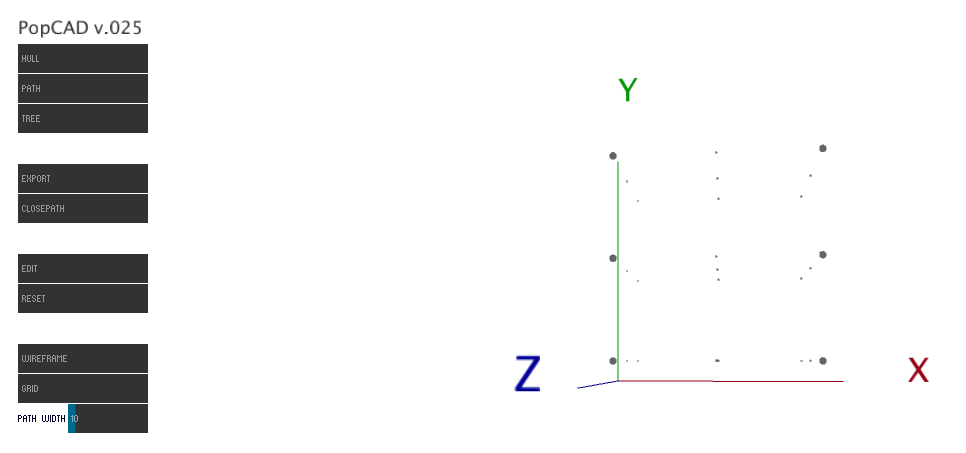
\includegraphics[width=.44\linewidth, height=1.6in]{images/edit1} &
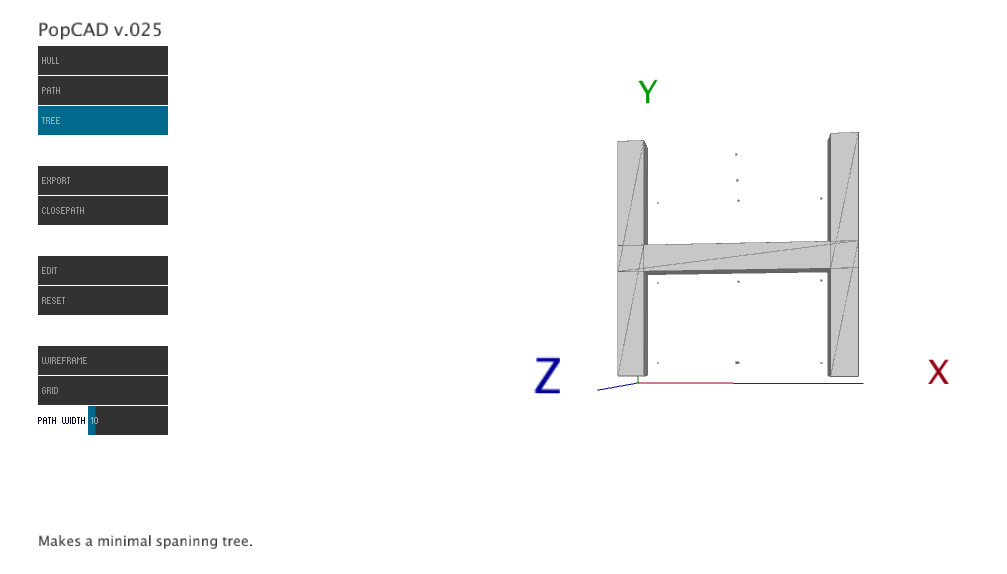
\includegraphics[width=.44\linewidth, height=1.6in]{images/edit2} \\
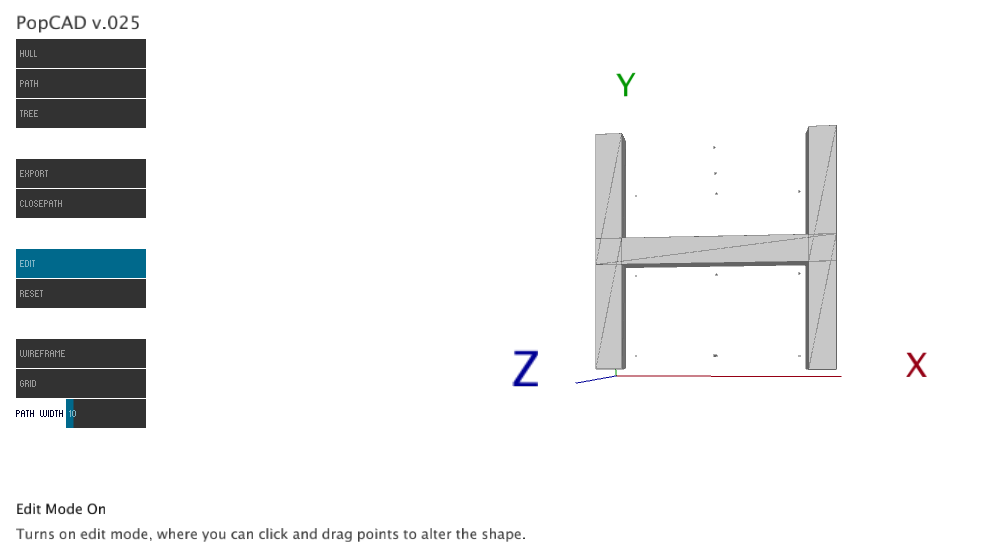
\includegraphics[width=.44\linewidth, height=1.6in]{images/edit3} &
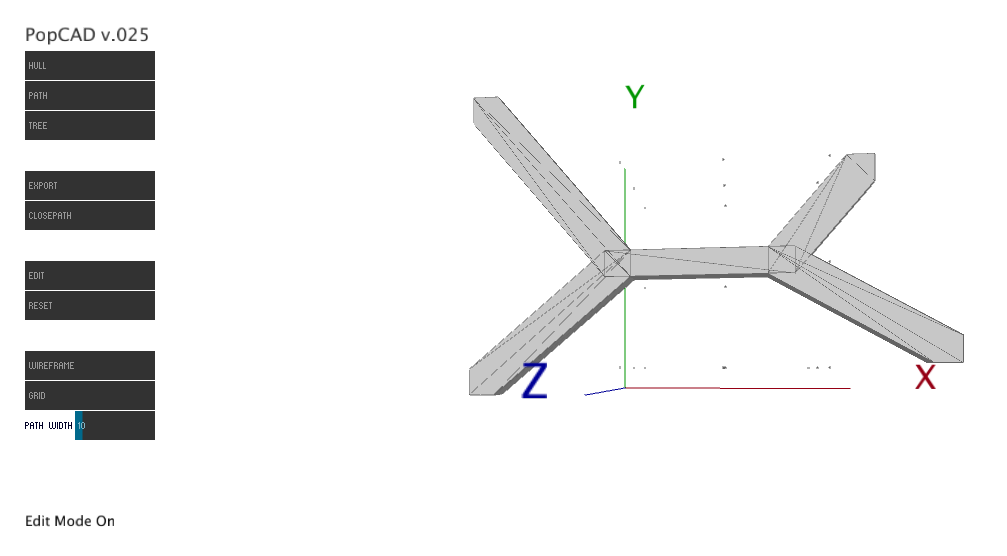
\includegraphics[width=.44\linewidth, height=1.6in]{images/edit4}
\end{array}$
\end{center}
\caption{A four step sequence showing the operation of the edit mode: (upper
left) six unaltered points; (upper right) the points form an ``H'' shape
with tree mode selected; (lower left) the selection of edit mode; (lower
right) the edited shape, with the corners of the original shape extended
outward.}
\label{fig:editMode}
\end{figure}

Figure \ref{fig:editMode} shows a four-step sequence of screen shots using the
edit mode to alter a shape: (upper left) six points have been lighted on the
PopCAD and are reflected as simple points in the software; (upper right) the
user has selected ``tree'' mode, taking the minimal spanning tree of the six
points, forming a sort of ``H'' pattern; (lower left) the user selects the
``edit mode'' button, freezing the serial input and initiating the
click-and-drag editing ability; (lower right) the user has dragged each of the
four ``corner'' points outward, altering the original shape into something new,
impossible to model using only the ``raw'' points available on the device.

\subsubsection{Stereolithography Export}

One of the most important functions of the software is to make a user's
creations into easily 3D-printable shapes. Many complex 3D software programs
allow for export into sterolithography format (.STL), which is the common input
format for 3D printer software programs, however, these programs rarely check to
ensure that the produced file will actually be printable; many ``model-able''
shapes will cause errors in 3D printer software - lines, 2D shapes, shapes
within shapes, shapes with gaps between faces - and on and on. Our software also
exports into .STL format, but takes great pains to ensure that any exported file
will print without error.

The export function in our software deals with models formed from all three
modes simply by keeping track of the active mode and choosing the correct export
method accordingly. The export process is similar for each type of shape: since
each shape is actually constructed of one or more convex hulls, the array of 3D
vectors describing (in order) each triangulated face of the hull (or hulls) is
added to a triangle mesh, which takes in all the faces, flips the Y axis
values for each coordinate (because in the Processing environment, (0,0) is in
the upper left), flips the vertex order, which corrects problems with sliceform
errors (in 3D printing software) resulting from the face normal vectors facing
the wrong way, then adds all the faces to an .STL object, which outputs a series
of triangles in an .STL file the describes the object.

\begin{figure}[!ht]
\begin{center}
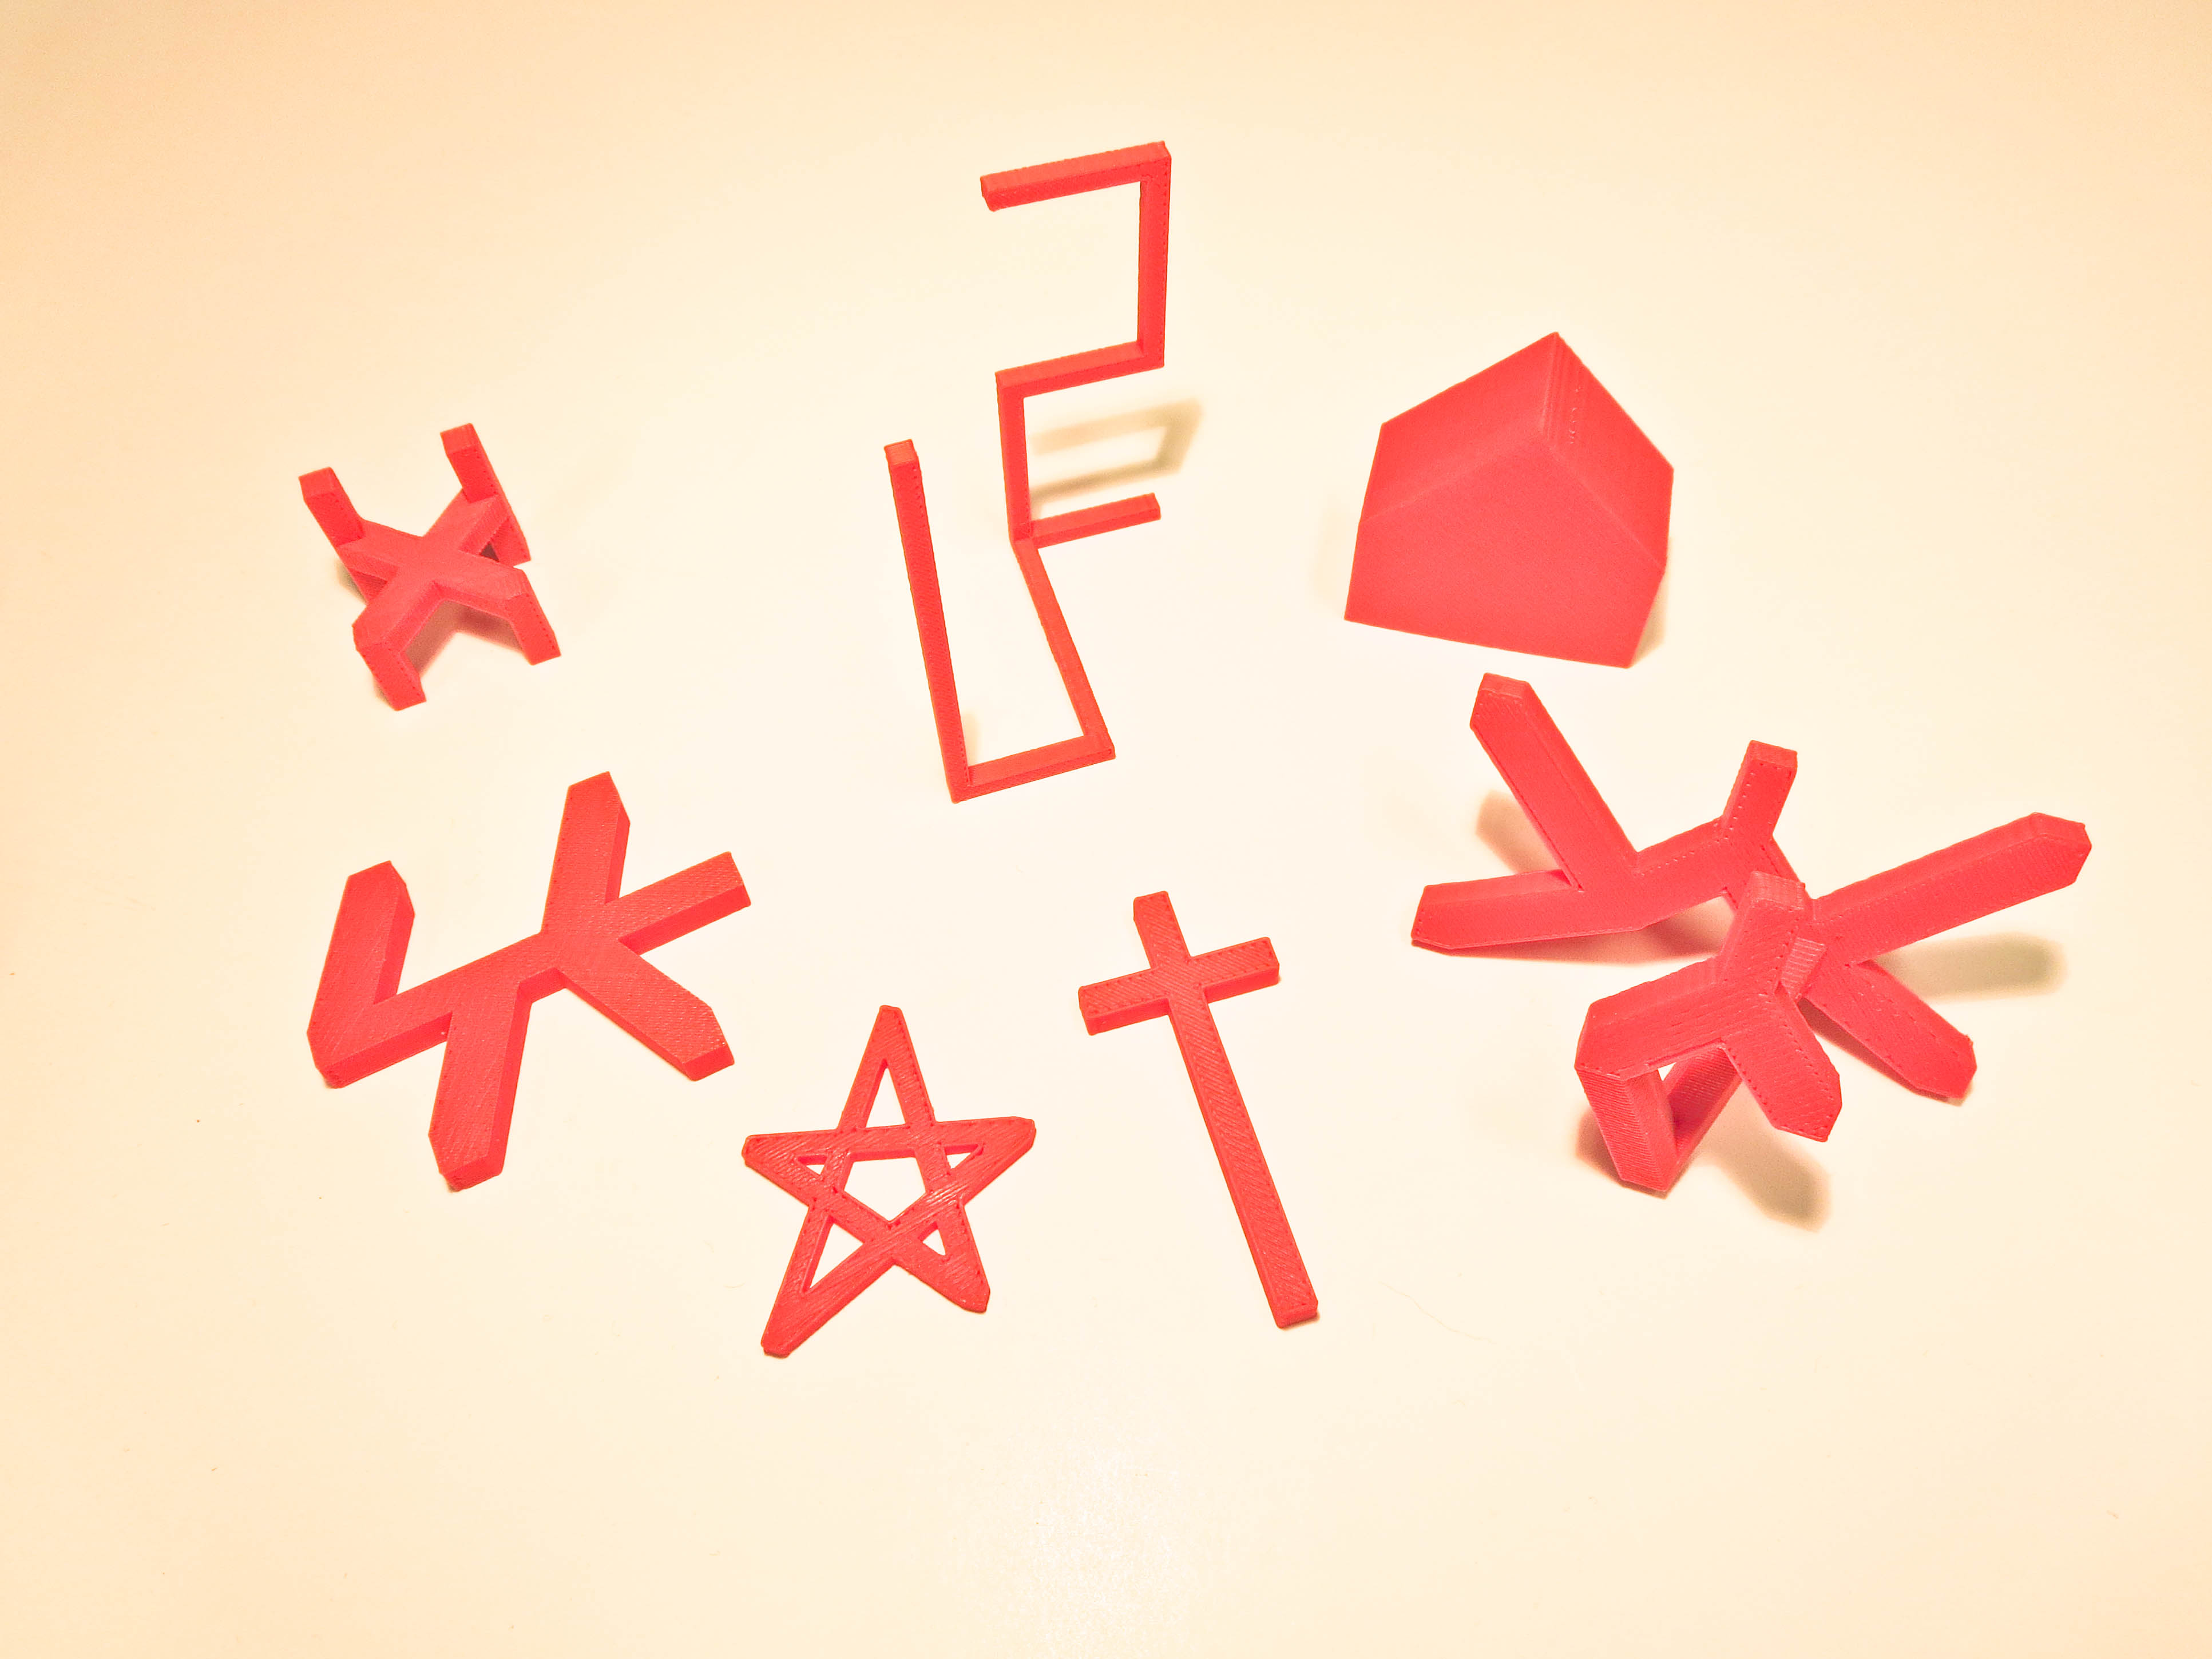
\includegraphics[width=.5\linewidth]{images/userShapes1}
\end{center}
\caption{Several of the shapes modeled on the PopCAD and SnapCAD devices by
novices designers (most of them without any previous 3D modeling expertise)
from one of the user studies we performed.}
\label{fig:userShapes1}
\end{figure}

Creating a ``novice-proof'' stereolithography export (all of the above
computation happens with one click, even the file naming) is crucial to the
raison d'\^{e}tre of our work - to democratize the process of designing
meaningful, personalized objects for 3D printing by novice designers. See Figure
\ref{fig:userShapes1} for a taste of what these novice designers are capable of
(more discussion of this occurs in later chapters, but a glimpse is far too
tempting to omit here).








